% ---- ETD Document Class and Useful Packages ---- %
\documentclass{ucetd}
\usepackage{booktabs}
\usepackage{amsfonts}
\usepackage{amsthm}
\usepackage{epsfig, minted}
%\usepackage[utf8x]{inputenc}
\usepackage{amsmath}
\let\Bbbk\relax
\usepackage{amssymb}
\usepackage{algorithm}
\usepackage{algorithmicx}
\usepackage[noend]{algpseudocode}
\usepackage{enumitem}      % adjust spacing in enums
%\usepackage{subfig}
\usepackage{caption}
\usepackage{subcaption}
\usepackage{multirow}
\usepackage{rotating}
\usepackage{wrapfig}
\usepackage{tabu}
\usepackage{cleveref}
\usepackage{array}
\usepackage{pifont}
\usepackage[normalem]{ulem}

%% Use these commands to set biographic information for the title page:
\title{Capitalizing on Security, Performance, and Energy Tradeoffs in Full Drive Encryption Schemes for Fun and Profit}
\author{Bernard Dickens III}
\department{Computer Science}
\division{Physical Sciences}
\degree{Doctor of Philosophy}
\date{July 2020}

%% Use these commands to set a dedication and epigraph text
\dedication{To my kiddos (whom at the time of writing do not yet exist): I find
the courage to peer over the edge of human knowledge and reach down into that
abyss of the unknown with the hope that you may one day benefit from my
struggles. I can't wait to meet you!}
%\epigraph{Epigraph Text}

%% Custom additions

%enumitem settings
\setlist{
  listparindent=\parindent,
  parsep=0pt,
}

% Fancy subsection references with cref
\crefformat{section}{\S#2#1#3} % see manual of cleveref, section 8.2.1
\crefformat{subsection}{\S#2#1#3}
\crefformat{subsubsection}{\S#2#1#3}

% Flexible table column specifications
\newcolumntype{C}[1]{>{\centering\arraybackslash}m{#1}}

\usepackage[natbib=true,backend=bibtex,firstinits=true,style=numeric-comp,sorting=nyt,defernumbers,maxnames=99,maxcitenames=99]{biblatex}
\usepackage{balance}
\usepackage{adjustbox}

\addbibresource{refs.bib}

\usepackage{pgfplots}

\pgfplotsset{compat=1.8,compat/show suggested version=false}
\usetikzlibrary{plotmarks}
\usetikzlibrary{calc}

\pgfplotsset{
   /pgfplots/bar  cycle  list/.style={/pgfplots/cycle  list={%
        {black,fill=black!30!white,mark=none},%
        {black,fill=red!30!white,mark=none},%
        {black,fill=green!30!white,mark=none},%
        {black,fill=yellow!30!white,mark=none},%
        {black,fill=brown!30!white,mark=none},%
     }
   },
}

\usetikzlibrary{external}
\tikzexternalize[prefix=out/]
\tikzexternalize

\usetikzlibrary{patterns}
\usepgfplotslibrary{groupplots}
\pgfplotsset{
   every axis label/.append style={font=\small},
   tick label style={font=\small},
}

\pgfkeys{
    /pgf/number format/precision=1,
    /pgf/number format/fixed zerofill=true,
}

%% Custom colors that are colorblind safe, print friendly, and photocopy safe
\definecolor{purpleDark}{RGB}{94, 60, 153}
\definecolor{purpleLight}{RGB}{178, 171, 210}
\definecolor{orangeDark}{RGB}{230, 97, 1}
\definecolor{orangeLight}{RGB}{253, 184, 99}

%% Other custom colors
\definecolor{gray}{gray}{0.75}

% Ability to filter the values plotted from tables via `discard if not` key
\pgfplotsset{
    discard if symbol/.style 2 args={
        x filter/.append code={
            \edef\tempa{\thisrow{#1}}
            \edef\tempb{#2}
            \ifx\tempa\tempb
                \def\pgfmathresult{inf}
            \fi
        }
    }
}

\pgfplotsset{
    discard if symbol not/.style 2 args={
        x filter/.append code={
            \edef\tempa{\thisrow{#1}}
            \edef\tempb{#2}
            \ifx\tempa\tempb
            \else
                \def\pgfmathresult{inf}
            \fi
        }
    }
}

\pgfplotsset{
    discard if number/.style 2 args={
        x filter/.append code={
            \ifdim\thisrow{#1} pt=#2pt
                \def\pgfmathresult{inf}
            \fi
        }
    }
}

\pgfplotsset{
    discard if number not/.style 2 args={
        x filter/.append code={
            \ifdim\thisrow{#1} pt=#2pt
            \else
                \def\pgfmathresult{inf}
            \fi
        }
    }
}

\pgfplotsset{
    nodes near coords greater equal only/.style={
        small value/.style={
            /tikz/coordinate,
        },
        every node near coord/.append style={
            check for small values/.code={
                \begingroup
                \pgfkeys{/pgf/fpu}
                \pgfmathparse{\pgfplotspointmeta<#1}
                \global\let\result=\pgfmathresult
                \endgroup
                \pgfmathfloatcreate{1}{1.0}{0}
                \let\ONE=\pgfmathresult
                \ifx\result\ONE
                    \pgfkeysalso{/pgfplots/small value}
                \fi
            },
            check for small values
        },
    },
}

\pgfplotsset{
    nodes near coords greater only/.style={
        small value/.style={
            /tikz/coordinate,
        },
        every node near coord/.append style={
            check for small values/.code={
                \begingroup
                \pgfkeys{/pgf/fpu}
                \pgfmathparse{\pgfplotspointmeta<=#1}
                \global\let\result=\pgfmathresult
                \endgroup
                \pgfmathfloatcreate{1}{1.0}{0}
                \let\ONE=\pgfmathresult
                \ifx\result\ONE
                    \pgfkeysalso{/pgfplots/small value}
                \fi
            },
            check for small values
        },
    },
}

\algnewcommand{\LineComment}[1]{\(\triangleright\) #1}

% some useful shortcuts
\newcommand{\ie}{\textit{i.e., }}
\newcommand{\eg}{\textit{e.g., }}
\newcommand{\CC}{C\nolinebreak\hspace{-.05em}\raisebox{.5ex}{\tiny\bf +}\nolinebreak\hspace{-.10em}\raisebox{.5ex}{\tiny\bf +}}

% units for results
\newcommand{\us}{\,$\mu$s}
\newcommand{\ms}{\,ms}
\newcommand{\KB}{\,KB}
\newcommand{\MB}{\,MB}
\newcommand{\GB}{\,GB}
\newcommand{\MHz}{\,MHz}
\newcommand{\GHz}{\,GHz}

% new latex commands:
%   Remove long section
\newcommand{\PUNT}[1]{}
\newcommand{\TABLETWO}[1]{}
%   Label work to be done
\definecolor{gray}{gray}{0.75}
\newcommand{\TODO}[1]{\textcolor{gray}{\textbf{\ [TODO:\ #1]\ }}}
\newcommand{\TR}[1]{#1}
%\newcommand{\TR}[1]{}
%\newcommand{\TODO}[1]{}
\newcommand{\FIX}[1] {\textcolor{red}{\textbf{\ [FIX:\ #1]\ }}}
%   Referencing various pieces of the document:
\newcommand{\figref}[1]{Fig.~\ref{fig:#1}}
\newcommand{\figsref}[2]{Figures~\ref{fig:#1} and~\ref{fig:#2}}
\newcommand{\figrref}[2]{Figures~\ref{fig:#1}--\ref{fig:#2}}
\newcommand{\secref}[1]{Section~\ref{sec:#1}}
\newcommand{\secsref}[2]{Sections~\ref{sec:#1} and~\ref{sec:#2}}
\newcommand{\eqnref}[1]{Eqn.~\ref{eqn:#1}}
\newcommand{\eqnsref}[2]{Equations~\ref{eqn:#1} and~\ref{eqn:#2}}
\newcommand{\eqnrref}[2]{Equations~\ref{eqn:#1}--\ref{eqn:#2}}
\newcommand{\insref}[1]{Instruction~\ref{ins:#1}}
\newcommand{\tblref}[1]{Table~\ref{tbl:#1}}
\newcommand{\appref}[1]{Appendix~\ref{app:#1}}

\newcommand{\algoref}[1]{Algorithm~\ref{algo:#1}}

\makeatletter
\newcommand\footnoteref[1]{\protected@xdef\@thefnmark{\ref{#1}}\@footnotemark}
\makeatother

% Custom hyphenation rules

%\DeclareMathOperator{\minimize}{minimize}
%\DeclareMathOperator{\st}{s.t.}
%\DeclareMathOperator*{\argmin}{arg\,min}
%\DeclareMathOperator*{\argmax}{arg\,max}
\newcommand{\argmin}{\arg\!\min}
\newcommand{\argmax}{\arg\!\max}
\newcommand{\minimize}{minimize}
\newcommand{\optimize}{optimize}
\newcommand{\ceil}[1]{\lceil #1 \rceil}
\newcommand{\floor}[1]{\lfloor #1 \rfloor}
\newcommand{\st}{s.t.}

\newcommand{\StrongBoxURI}{https://github.com/Xunnamius/strongbox-switchcrypt}
\newcommand{\SwitchCryptURI}{https://github.com/Xunnamius/strongbox-switchcrypt}

% \pdfstringdefDisableCommands{
%     \def\\{}
%     \def\unskip{}
%     \def\texttt#1{<#1>}
% }

%-------------------------------------------------------------------------

\begin{document}
%% Basic setup commands
% If you don't want a title page comment out the next line and uncomment the line after it:
\maketitle
%\omittitle

% These lines can be commented out to disable the copyright/dedication/epigraph pages
\makecopyright
\makededication
% \makeepigraph

%% Make the various tables of contents
\tableofcontents
\listoffigures
\listoftables

\acknowledgments
I would first and foremost like to thank my advisor, Dr. Henry (Hank) Hoffmann.
Without your compassion, patience, conscientiousness, and cosmic wealth of
knowledge and experience, none of this work would have been possible. Thank you
for everything you've done for my students and me. You are truly a rare ally.

I'd like to thank my committee members Dr. Ariel J. Feldman (Applied Crypto),
Dr. Haryadi S. Gunawi (Filesystems), and Dr. David Cash (Theoretical Crypto) for
all their hours of hard work and tireless dedication even in the middle of a
pandemic. I learned so much studying under you. Hopefully I spelled everyone's
names correctly this time, haha!

I'd also like to acknowledge my former students Richard Anthony Alvarez and
Trevor James Medina for their huge contributions to HASCHK and to my sanity.
Equally important are Abraham Valle (a fullstack flexer!), Mark Alvarez
(remember the name, it'll be on a ballot some day), Malik Swanson, Michael
Desiderio, former students Tyrese Cook, Rakim Jazz Verner, Ephriam, Matthew,
Malcolm, Byron, Leroy, and all the others... I love you guys.

I'd be remiss if I did not acknowledge the pivotal role played by my lovely
hyper-intelligent mother (I had to get it from somewhere) Michelle Davis who,
throughout my childhood, \emph{always} had money for Computer Science workbooks
(but somehow not McDonalds!); as well as my father Bernard Dickens II for always
taking the extra effort to be there for me and always with my best interests at
heart. Thank yous also go out to: my inspiring siblings Davis and Milan; Zara
for the infinity life lessons---you were my rock, my reality hook; Jeff Holmes
of the old Chicago Broadway Armory for showing an eight-year-old me just how fun
and powerful \sout{hacking} computers can be; Von Steuben high school Computer
Science teachers Stirling Crow and Andres Hernandez for teaching me web design
and gifting me the wisdom to ``use my CS powers for good;'' my coach Audra
Anderson and the BDPA for teaching me humility and how fulfilling it is to be an
engaging teacher and effective helper; Dr. Rahmelle Thompson of the Morehouse
College Hopps Scholars program for revealing my trajectory to me; Dr. Adrienne
Raglin of the Department of Defense Army Research Laboratory for putting up with
me (twice!) and teaching me what real research looks like; neighborhood
matriarch Martha Alvarez for looking out for me during my last few years in
Chicago; the University of Chicago and all its faculty and staff for fostering a
culture of socially conscious elite intellectual pursuit; President Barack H.
Obama and Senator Elizabeth Warren for demonstrating black excellence and how to
persist nevertheless; and all my mentors, former students, and true friends over
the years for their unwavering support throughout this process. Know I would not
have made it without every last one of you.

I must give special thanks to my UChicago family: Connor. Our interactions were
usually brief, but you blazed the trail for me in particular... I was so nervous
(my default state!) but hearing you talk about your experiences
post-M.S.-defense really helped me calm down and focus. Thank you and Saeid for
all your wisdom. Anne, thanks for listening to my boring talk! Your feedback
during the group meeting really helped hone my presentation. Ivana and Will,
thank you for reaching out! I'm just a hopeless recluse. Kavon, our
conversations were fun. Huazhe would greet me on those rare occasions I entered
the office... thank you for the warm welcomes! Nikita, Yi, Santriaji, Yuli,
Tejas, Ahsan, it was my pleasure to get to know you all.

This material is based upon work supported by the National Science Foundation
under Grant No. CNS-1526304. So thank you too United States discretionary
spending budget authorized by Congress.

\abstract
The security of data at rest---widely understood as FDE or Full-Drive
Encryption---is an important concern among several in modern computer systems.
These concerns exist in contention over a set of finite resources. For instance:
a device that is battery-constrained must remain within its energy budget which
may change over time, e.g. when a device enters ``battery-saver mode'';
regardless, this device must meet certain performance guarantees or the user
experience will suffer; above all, the data on the device must be secure from
adversaries; and the device has a finite amount of drive space available. At any
given moment we trade battery life for performance, performance for security,
security for drive space, and so on. Unfortunately, designing a FDE system that
can navigate such treacherous tradeoffs efficiently, effectively, and with
respect to performance and security guarantees is entirely non-trivial. This
dissertation explores this space of tradeoffs and how we might optimize for one
concern without violating another given kernel and/or user space in-context
invariants that might shift over time.

Full-drive encryption is especially important for mobile devices because they
contain large quantities of sensitive data yet are easily lost or stolen. As
this research demonstrates, the standard approach to FDE—the AES block cipher in
XTS mode—is 3-5x slower than unencrypted storage. Authenticated encryption based
on stream ciphers is already used as a faster alternative to AES in other
contexts, such as HTTPS, but the conventional wisdom is that stream ciphers are
unsuitable for FDE. Used naively in drive encryption, stream ciphers are
vulnerable to attacks, and mitigating these attacks with on-drive metadata is
generally believed to ruin performance.

We address the difficulty of using stream ciphers for FDE with StrongBox, a
stream cipher based FDE layer that is a drop-in replacement for dm-crypt, the
standard Linux FDE module based on AES-XTS. StrongBox introduces a system design
and on-drive data structures that exploit certain properties of filesystems to
avoid costly rekeying penalties and a counter stored in trusted hardware to
protect against attacks. We implement StrongBox and SwitchCrypt on an ARM
big.LITTLE mobile processor and test its performance under multiple popular
production filesystems.

We push the envelope further with SwitchCrypt, a software mechanism that allows
us to move beyond merely making stream ciphers available for FDE. SwitchCrypt
enables practical navigation of the tradeoff space made by balancing competing
security and latency requirements via \emph{cipher switching} in space or time.
Our key insight in achieving low-overhead switching is to leverage the
overwrite-averse, append-mostly behavior of underlying solid-state storage to
trade throughput for reduced energy use and/or certain security properties.
Similar to StrongBox, we implement SwitchCrypt on an ARM big.LITTLE mobile
processor and test its performance under the popular F2FS LFS. We provide
empirical results demonstrating the conditions under which different switching
strategies are optimal through the exploration of four cases studies.

Finally, with HASCHK, we consider the same stream cipher based cryptographic
primitives in an alternative domain: data \emph{in motion} rather than at rest.
Specifically: securing data downloads over the internet. Such downloads come
with many risks, including the chance that the resource has been corrupted, or
that an attacker has replaced your desired resource with a compromised version.
The de facto standard for addressing this risk is the use of \emph{checksums}
coupled with a secure transport layer; users download a resource, compute its
checksum, and compare that with an authoritative checksum. Problems with this
approach include (1) \emph{user apathy}---for most users, calculating and
verifying the checksum is too tedious; and (2) \emph{co-hosting}---an attacker
who compromises a resource can trivially compromise a checksum hosted on the
same system. The co-hosting problem remains despite advancements in tools that
automate checksum verification and generation. In this dissertation we propose
\emph{HASCHK}, a resource verification protocol expanding on de facto
checksum-based integrity protections to defeat co-hosting while automating the
tedious parts of checksum verification to secure ``data in motion'' over the
internet.

StrongBox, SwitchCrypt, and HASCHK together demonstrate that security is indeed
a paramount concern and valid dimension with which to trade off alongside other
tier-one concerns without compromising data security or requiring obscene
performance sacrifices, all while staying within a shifting energy budget.


\mainmatter
% Main body of text follows

\chapter{Introduction} \label{chp:introduction}

In this section we make our thesis statement, describe the problem StrongBox
solves, and outline the general StrongBox approach.

\section{Thesis Statement}

With this research into filesystem, device driver, and hardware Flash
Translation Layer (FTL) based Full Disk Encryption (FDE) schemes, we primarily
consider: (1) the established wisdom in the crypto community that stream ciphers
are unsuitable for FDE and (2) exploring the tradeoff space made between total
energy use, filesystem performance, and reasonable security guarantees when
comparing specific cipher configurations. In the first case, we develop and
implement a secure approach to FDE based on stream ciphers, the proliferation of
secure hardware, and the characteristics of Log-Structured Filesystems (LFS). In
the second case, we implement a dozen stream ciphers---each exposing several
knobs---and demonstrate navigating our tradeoff space via runtime cipher
switching while maintaining reasonable security guarantees. We then present a
formal analysis of our system's security guarantees.

\section{Problem Description}

Full-drive encryption (FDE)\footnote{The common term is full-\emph{disk}
encryption, but this work targets SSDs, so we use \emph{drive}.} is an essential
technique for protecting the privacy of data at rest. For mobile devices,
maintaining data privacy is especially important as these devices contain
sensitive personal and financial data yet are easily lost or stolen. The current
standard for securing data at rest is to use the AES cipher in XTS
mode~\cite{XTS, NISTXTS}. Unfortunately, employing AES-XTS increases read/write
latency by 3--5$\times$ compared to unencrypted storage.

It is well known that authenticated encryption using \emph{stream}
ciphers---such as ChaCha20~\cite{ChaCha20}---is faster than using AES. Indeed,
Google made the case for stream ciphers over AES, switching HTTPS connections on
Chrome for Android to use a stream cipher for better
performance~\cite{google-blog}. Stream ciphers are not used for FDE, however,
for two reasons: (1) confidentiality and (2) performance. First, when applied
naively to stored data, stream ciphers are trivially vulnerable to
attacks---including \emph{many-time pad and rollback attacks}---that reveal the
plaintext by overwriting a secure storage location with the same key. Second, it
has been assumed that adding the meta-data required to resist these attacks
would ruin the stream cipher's performance advantage. Thus, the conventional
wisdom is that FDE necessarily incurs the overhead of AES-XTS or a similar
primitive.

We argue that two technological shifts in mobile device hardware overturn this
conventional wisdom, enabling confidential, high-performance storage with stream
ciphers. First, these devices commonly employ solid-state storage with Flash
Translation Layers (FTL), which operate similarly to Log-structured File Systems
(LFS)~\cite{LFS,F2FS,NILFS}. Second, mobile devices now support trusted
hardware, such as Trusted Execution Environments (TEE)~\cite{TEE,TrustZone} and
secure storage areas~\cite{eMMC-standard}. FTLs and LFSes are used to limit
sector/cell overwrites, hence extending the life of the drive. Most writes
simply appended to a log, reducing the occurrence of overwrites and the chance
for attacks. The presence of secure hardware means that drive encryption modules
have access to persistent, monotonically increasing counters that can be used to
prevent rollback attacks when overwrites do occur.

Given these trends, we propose StrongBox, a new method for securing data at
rest. StrongBox is a drop-in replacement for AES-XTS-backed FDE such as
dm-crypt~\cite{dmcrypt}; i.e. it requires no interface changes. The primary
challenge is that even with a FTL or LFS running above an SSD, filesystem blocks
will occasionally be overwritten; e.g. by segment cleaning or \emph{garbage
collection}. StrongBox overcomes this challenge by using a fast stream cipher
for confidentiality and performance with integrity preserving Message
Authentication Codes~\cite{MAC} or ``MAC tags'' and a secure, persistent
hardware counter to ensure integrity and prevent attacks. \emph{StrongBox's main
contribution is a system design enabling the first confidential,
high-performance drive encryption based on a stream cipher.}

\section{Related Work} \label{sec:hc-related}

In this section, we examine prior approaches to guaranteeing resource integrity
over the internet. We then highlight some drawbacks to these approaches and how
HASCHK differs. \\

\noindent\textbf{Anti-malware software, heuristics, and blacklists.}
Anti-malware software is a heuristic-based program designed for the specific
purpose of detecting and removing various kinds of malware. However, updates to
anti-malware definitions often lag behind or occur in response to the release of
crippling malware. For example, during the 2017 compromise of the HandBrake
distribution mirror, users who first ran the compromised HandBrake image through
\textit{VirusTotal}---a web service that will run a resource through several
dozen popular anti-malware products---received a report claiming no infections
were detected despite the presence of the Proton malware~\cite{SCA-HB1}. In the
2012 compromise of SourceForge's CDN, the malicious changes to the phpmyAdmin
image do not appear as malware to anti-malware software~\cite{SCA-PMA1}.

Similarly, all modern browsers employ heuristic and blacklist-based detection
and prevention schemes in an attempt to protect users from malicious content on
the internet. The warnings generated by browser-based heuristics and blacklists
are also reactive rather than proactive; hence, they are generally ineffective
at detecting active or novel attacks on the integrity of the resources
downloaded over the internet.

On the other hand, HASCHK relies on no heuristics or blacklists and is not
anti-malware software. HASCHK is a protocol for automating checksum
verification of resources. This ensures download integrity---that a user is
receiving the expected resource a provider is advertising---not that the
expected resource is not malware. \\

\noindent\textbf{Link Fingerprints and Subresource Integrity.} The Link
Fingerprints (LF) draft describes an early HTML hyperlinks and URI based
resource integrity verification scheme that ``provides a backward-compatible
technique for resource providers to ensure that the resource originally
referenced is the same as the resource retrieved by an end user.''~\cite{LF}.
The World Wide Web Consortium's (W3C) Subresource Integrity (SRI) describes a
similar HTML-based scheme designed exclusively with CDNs and web assets in mind.

Like HASCHK, both LF and SRI employ cryptographic digests to ensure no
changes of any kind have been made to a resource~\cite{SRI}. Unlike HASCHK,
LF and SRI apply \emph{only to resources referenced by script and link HTML
elements}; HASCHK, on the other hand, can ensure the integrity of \emph{any
arbitrary resource downloaded over the internet}, even outside of HTML web pages
and browser software. Further, the checksums contained in the HTML source must
be accurate for SRI to work. If the system \emph{behind} the CDN is compromised,
the attacker can alter the HTML and inject a malicious checksum or even strip
checksums from the HTML entirely. With HASCHK, however, an attacker would
additionally have to compromise the separate backend system that advertises the
provider's resources, thus raising the bar. \\

\noindent\textbf{Content-MD5 Header.} The Content-MD5 header field is a
deprecated email and HTTP header that delivers a checksum similar to those used
by Subresource Integrity. It was removed from the HTTP/1.1 specification because
of the inconsistent implementation of partial response handling between
vendors~\cite{HTTP1.1}. Further, the header could be easily stripped off or
modified by proxies and other intermediaries~\cite{MD5Header}. HASCHK
exhibits none of these weaknesses. \\

\noindent\textbf{Deterministic Build Systems and Binary Transparency.} A
deterministic build system is one that, when given the same source, will
deterministically output the same binary on every run. For example, many
packages in Debian~\cite{ReproBuildsDebian} and Arch Linux can be rebuilt from
source to yield an identical byte for byte result~\cite{ReproBuilds}, allowing
for verification of the \emph{Integration} and perhaps \emph{Development} supply
chain phases (see \tblref{attacks}). Further, using a merkle
tree~\cite{MerkleTree} or similar construction, an additional chain of trust can
be established that allows for public verification of the \emph{Deployment},
\emph{Maintenance}, and \emph{Retirement} supply chain phases. Companies such as
Mozilla refer to the latter as ``Binary Transparency.''

Like HASCHK, binary transparency establishes a public verification scheme
that allows third party consumers access to a listing of source updates
advertised by a provider~\cite{BinaryTransparency}. Consumers can leverage
deterministic build systems and Binary Transparency together to ensure their
software is the same software deployed to every other system. Unlike HASCHK,
binary transparency only allows a user to verify the integrity of \emph{source
updates to binaries}; our protocol allows a user to verify the integrity of
\emph{any arbitrary resource} while specifically addressing co-hosting. \\

\noindent\textbf{Stickler and Cherubini et al.} Stickler~\cite{Stickler} by Levy
et al. is an automated JavaScript-based stand-in for SRI for protecting the
integrity of web application files hosted on CDNs. Stickler does not require any
modifications to the client (\ie{ a frontend}), instead delivering a bootloader
to load and verify resources signed before the fact. However, as it was designed
to stand-in for SRI, Stickler inherits some of SRI's limitations. Specifically:
Stickler was not designed to protect arbitrary resource downloads and, if the
publisher's server is compromised, Stickler's bootloader can be stripped out of
the initial HTTP response altogether. Something like this is not possible with
HASCHK.

The automated checksum verification approach described by Cherubini et
al.~\cite{Cherubini}, also based on SRI, is similarly vulnerable to (and relies
upon) co-hosting. Cherubini's browser extension works by both looking for
embedded checksums in download links (SRI) and extracting hexadecimal strings
that look like checksums directly from the HTML source. An attacker, after
compromising the resource file, need only modify the provider's HTML file to
inject a corrupted ``integrity'' attribute containing a checksum matching that
corrupted resource, causing Cherubini's extension to misreport the dangerous
download as safe~\cite{Cherubini}. Additionally, Cherubini's extension: (1) does
not alert users when corresponding authoritative checksums are not found, which
means an attacker can simply strip all checksums from the server response to
pass off compromised resources to users; (2) considers a download ``safe'' so
long as \emph{any checksum found on the page matches it}, which means an
attacker can just inject the compromised checksum somewhere in the HTML source
alongside the legitimate checksum to similarly pass off compromised resources to
users; (3) does not support direct downloads, \ie{ when a user enters a
resource's URI into the browser manually rather than click a hyperlink}. None of
this is a problem for HASCHK.


\chapter{StrongBox: Using Stream Ciphers for High Performance Full Drive Encryption} \label{chp:strongbox}
\section{Motivation} \label{sec:sb-motivation}

Full-drive encryption (FDE) is especially important for mobile devices because
they contain large quantities of sensitive data yet are easily lost or stolen.
Unfortunately, the standard approach to FDE---the AES block cipher in XTS
mode---is 3--5x slower than unencrypted storage. Authenticated encryption based on
stream ciphers is already used as a faster alternative to AES in other contexts,
such as HTTPS, but the conventional wisdom is that stream ciphers are unsuitable
for FDE. Used naively in drive encryption, stream ciphers are vulnerable to
attacks, and mitigating these attacks with on-drive metadata is generally
believed to ruin performance.

In this paper, we argue that recent developments in mobile hardware invalidate
this assumption, making it possible to use fast stream ciphers for FDE. Modern
mobile devices employ solid-state storage with Flash Translation Layers (FTL),
which operate similarly to Log-structured File Systems (LFS). They also include
trusted hardware such as Trusted Execution Environments (TEEs) and secure
storage areas. Leveraging these two trends, we propose StrongBox, a stream
cipher-based FDE layer that is a drop-in replacement for dm-crypt, the standard
Linux FDE module based on AES-XTS. StrongBox introduces a system design and
on-drive data structures that exploit LFS's lack of overwrites to avoid costly
rekeying and a counter stored in trusted hardware to protect against attacks. We
implement StrongBox on an ARM big.LITTLE mobile processor and test its
performance under multiple popular production LFSes. We find that StrongBox
improves read performance by as much as $2.36\times$ ($1.72\times$ on average)
while offering stronger integrity guarantees.

Full-drive encryption (FDE)\footnote{The common term is full-\emph{disk}
encryption, but this work targets SSDs, so we use \emph{drive}.} is an essential
technique for protecting the privacy of data at rest. For mobile devices,
maintaining data privacy is especially important as these devices contain
sensitive personal and financial data yet are easily lost or stolen. The current
standard for securing data at rest is to use the AES cipher in XTS
mode~\cite{XTS, NISTXTS}. Unfortunately, employing AES-XTS increases
read/write latency by 3--5$\times$ compared to unencrypted storage.

It is well known that authenticated encryption using \emph{stream}
ciphers---such as ChaCha20~\cite{ChaCha20}---is faster than using AES (see
\figref{motivation}). Indeed, Google made the case for stream ciphers over AES,
switching HTTPS connections on Chrome for Android to use a stream cipher for
better performance~\cite{google-blog}. Stream ciphers are not used for FDE,
however, for two reasons: (1) confidentiality and (2) performance. First, when
applied naively to stored data, stream ciphers are trivially vulnerable to
attacks---including \emph{many-time pad and rollback attacks}---that reveal the
plaintext by overwriting a secure storage location with the same key. Second, it
has been assumed that adding the meta-data required to resist these attacks
would ruin the stream cipher's performance advantage. Thus, the conventional
wisdom is that FDE necessarily incurs the overhead of AES-XTS or a similar
primitive.

We argue that two technological shifts in mobile device hardware overturn this
conventional wisdom, enabling confidential, high-performance storage with stream
ciphers. First, these devices commonly employ solid-state storage with Flash
Translation Layers (FTL), which operate similarly to Log-structured File Systems
(LFS)~\cite{LFS,F2FS,NILFS}. Second, mobile devices now support trusted
hardware, such as Trusted Execution Environments (TEE)~\cite{TEE,TrustZone} and
secure storage areas~\cite{eMMC-standard}. FTLs and LFSes are used to limit
sector/cell overwrites, hence extending the life of the drive. Most writes
simply appended to a log, reducing the occurrence of overwrites and the chance
for attacks. The presence of secure hardware means that drive encryption modules
have access to persistent, monotonically increasing counters that can be used to
prevent rollback attacks when overwrites do occur.

Given these trends, we propose StrongBox, a new method for securing data at
rest. StrongBox is a drop-in replacement for AES-XTS-backed FDE such as
dm-crypt~\cite{dmcrypt}; \ie it requires no interface changes. The primary
challenge is that even with a FTL or LFS running above an SSD, filesystem blocks
will occasionally be overwritten; \eg by segment cleaning or \emph{garbage
collection}. StrongBox overcomes this challenge by using a fast stream cipher
for confidentiality and performance with integrity preserving Message
Authentication Codes~\cite{MAC} or ``MAC tags'' and a secure, persistent
hardware counter to ensure integrity and prevent attacks. \emph{StrongBox's main
contribution is a system design enabling the first confidential, high-
performance drive encryption based on a stream cipher.}

We demonstrate StrongBox's effectiveness on a mobile ARM big.LITTLE system---a
Samsung Exynos Octa 5---running Ubuntu Trusty 14.04 LTS, kernel 3.10.58. We use
ChaCha20~\cite{ChaCha20} as our stream cipher, Poly1305~\cite{Poly1305} as our
MAC algorithm, and the eMMC Replay Protected Memory Block partition to store a
secure counter \cite{eMMC-standard}. As StrongBox requires no change to any
existing interfaces, we benchmark it on two of the most popular LFSes:
NILFS~\cite{NILFS} and F2FS~\cite{F2FS}. We compare the performance of these
LFSes on top of AES-XTS (via dm-crypt) and StrongBox. Additionally, we compare
the performance of AES-XTS encrypted Ext4 filesystems with StrongBox and F2FS.
Our results show:

\begin{itemize}

  \item \emph{Improved read performance:} StrongBox provides decreased read
latencies across all tested filesystems in the majority of benchmarks when
compared to dm-crypt; \eg under F2FS, StrongBox provides as much as a
$2.36\times$ ($1.72\times$ average) speedup over AES-XTS\@.

  \item \emph{Equivalent write performance:} despite having to maintain more
metadata than FDE schemes based on AES-XTS, StrongBox achieves near parity or
provides an improvement in observed write latencies in the majority of
benchmarks; \eg under F2FS, StrongBox provides an average $1.27\times$ speedup
over AES-XTS\@.

\end{itemize}

StrongBox achieves these performance gains while providing a stronger integrity
guarantee than AES-XTS\@. Whereas XTS mode only hopes to randomize plaintext when
the ciphertext is altered~\cite{XTS}, StrongBox provides the security of
standard authenticated encryption. In addition, StrongBox's implementation is
available open-source.\footnote{\StrongBoxURI}

\subsection{Performance Potential}

We demonstrate the potential performance win from switching to a stream cipher
by comparing AES-XTS to ChaCha20+ Poly1305. We use an Exynos Octa processor with
an ARM big.LITTLE architecture---the same processor used in the Samsung Galaxy
line of phones. We encrypt and then decrypt 250MB of randomly generated bits 3
times and take the median time for each of encryption and decryption.
\figref{motivation} shows the distinct advantage of the stream cipher over
AES---a consistent $2.7\times$ reduction in run time.

\begin{figure}[t]
  \begin{tikzpicture}

\begin{groupplot}[
    group style={
        group name=plots,
        group size=1 by 1,
        xlabels at=edge top,
        xticklabels at=edge top,
        vertical sep=5pt
    },
axis x line* = top,
xlabel near ticks,
major x tick style = transparent,
height=3.5cm,
%width=0.95\columnwidth,
width=4.2cm,
xmin=0,
xmax=3,
enlargelimits=false,
tick align = outside,
tick style={white},
ytick=\empty,
xtick=\empty,
xticklabels={},
yticklabels={},
]
\nextgroupplot[ylabel={\footnotesize Time (s)},
ylabel shift={6mm},
ymin=0,
ymax=1,
]


\end{groupplot}

\begin{groupplot}[
    group style={
        group name=plots,
        group size=1 by 1,
        xlabels at=edge bottom,
        xticklabels at=edge bottom,
        vertical sep=5pt
    },
axis x line* = bottom,
xlabel near ticks,
major x tick style = transparent,
height=3.5cm,
%width=0.95\columnwidth,
width=4.2cm,
xmin=0,
xmax=3,
enlargelimits=false,
tick align = outside,
tick style={white},
ytick=\empty,
xticklabel shift={-5pt},
%x tick label style={rotate=0, anchor=south},
%xlabel={\footnotesize $Platform$}
xtick={1,2},
xticklabels={{\scriptsize $\mathsf{Encrypt}$},
{\scriptsize $\mathsf{Decrypt}$}},
ymin=0,
ymax=50,
ytick={0,12.5,25,37.5,50},
yticklabels={0,,25,,50},
legend cell align=left, 
legend style={ column sep=1ex },
ymajorgrids,
grid style={dashed},
]
\nextgroupplot[ybar=\pgflinewidth,
bar width=5pt,
legend entries = {{\scriptsize $\mathsf{AES-XTS}$},
{\scriptsize $\mathsf{ChaCha+Poly1305}$}
},
legend style={draw=none,legend columns=2,at={(0.5,1.35)},anchor=north},
]
\addplot table[x index=0,y index=4, col sep=space] {img/heuristics2.txt};
\addplot table[x index=0,y index=5, col sep=space] {img/heuristics2.txt};


\end{groupplot}

\end{tikzpicture}

\caption{AES-XTS and ChaCha20+Poly1305 Comparison.} \label{fig:motivation}
\end{figure}

\subsection{Append-mostly Filesystems}
Of course, stream ciphers are not designed to encrypt data at rest.
If we naively implement block device encryption with a stream cipher,
overwriting the same memory location with the same key would trivially
allow an attacker to recover the secret key. Thus we believe stream
ciphers are best suited for encrypting block devices backing
Log-structured File Systems (LFSes), as these filesystems are designed
to append data to the end of a log rather than overwrite data. In
practice, some overwrites occur; \eg in metadata, but they are small
in number during normal execution.

To demonstrate this fact, we write 800MB of random data directly to the backing
store using four different file systems: Ext4, LogFS, NILFS, and F2FS. We count
the number of total writes to the underlying block device and the number of
times data is overwritten for each file system.


\begin{table}[th]
%\begin{wraptable}{r}{4cm}
\caption{File System Overwrite Behavior} \label{tbl:overwrites}
\footnotesize
\centering
\begin{tabular}{lrr}
  \textbf{File System} & \textbf{Total Write Ops} & \textbf{Overwrites} \\
  \hline
  \hline
  ext4    &  16,756 & 10,787\\
  LogFS   &   4,244 &     32\\
  NILFS   &   4,199 &     24\\
  F2FS    &   2.107 &      2\\
  \hline 
  \hline
\end{tabular}
%\vskip -.7em
%\end{wraptable}
\end{table}

\tblref{overwrites} shows the data for this experiment. Ext4 has the highest
number of writes, but many of those are small writes for book-keeping purposes.
Ext4 also has the largest number of overwrites. Almost 65\% of the writes are to
a previously written location in the backing store. In contrast, all three
Log-structured file systems have very few overwrites.

\subsection{Threat Model}

A stream cipher can be more than twice as fast as AES-XTS while providing the
same confidentiality guarantee. The problem is that a stream cipher is not
secure if the same key is used to overwrite the same storage location.
Fortunately, FTLs and LFSes rarely overwrite the same location.

We cannot, however, ignore the fact that overwrites do occur. While
\tblref{overwrites} shows overwrites are rare during normal operation, we know
they will occur when garbage collecting the LFS. Thus, we will need some
metadata to track writes and ensure that data is handled securely if overwrites
occur. Therefore, we recognize three key challenges to replacing AES with a
stream cipher for FDE:

\begin{itemize}

\item Tracking writes to the block device to ensure that the same location is
never overwritten with the same key.

\item Ensuring that the metadata that tracks writes is secure and is not
subject to leaks or rollback attacks.

\item Accomplishing the above efficiently so that we maintain the  performance
advantage of the stream cipher.

\end{itemize}

The key to StrongBox is using a secure, persistent counter supported in modern
mobile hardware; \eg for limiting password attempts. This counter can track
writes, and thus \emph{versions} of the encrypted data. If an attacker tried to
\emph{roll back} the file system to overwrite the same location with the same
key, our StrongBox detects that the local version number is out of sync with the
global version number stored in the secure counter. In that case, StrongBox
refuses to initialize and the attack fails. The use of the hardware-supported
secure counter significantly raises the bar when it comes to rollback attacks,
requiring a costly and non-discrete physical attack on the hardware itself to be
effective. The actual structure of the metadata required to track writes and
maintain integrity is significantly more complicated than simply implementing a
counter and is the subject of the next section.

An additional challenge is that of crash recovery. StrongBox relies on the
overlying filesystem to manage data recovery in the event of a crash that leaves
user data in an inconsistent state. StrongBox handles metadata recovery after a
crash by giving the root user the option to accept the current metadata state as
the new consistent state, \ie{``force mounting''}. This allows the root user to
mount the filesystem and access data after an unexpected shutdown. An attacker
might try to take advantage of this feature by modifying the backing store,
forcing an inconsistent state, and hoping the root user will ignore it and force
mount the system anyway. StrongBox defends against this attack by preventing
force mounts when metadata state is wildly inconsistent with the global version
counter. Otherwise, the root user is warned if they attempt a force mount. Thus,
attacking StrongBox by forcing a crash can only be successful if the attacker
also has root permission, in which case security is already compromised. Crash
recovery is also detailed in the next section.

\section{Related Work} \label{sec:sb-related}

Some of the most popular cryptosystems offering a confidentiality
guarantee for data at rest employ a symmetric encryption scheme known
as a Tweakable Enciphering Scheme (TES)~\cite{STES,XEX}. There have
been numerous TES-based constructions securing data at
rest~\cite{STES,CMC,HCTR}, including the well known XEX-based XTS
operating mode of AES~\cite{XTS} explored earlier in this work. Almost
all TES constructions and the storage management systems that
implement them use one or more block ciphers as their primary
primitive~\cite{TES-From-Stream-Cipher,STES}.

Our StrongBox implementation borrows from the design of these systems. One in
particular is \emph{dm-crypt}, a Linux framework employing a
\textit{LinuxDeviceMapper} to provide a virtual block interface for physical
block devices. Dm-crypt provides an implementation of the AES-XTS algorithm among
others and is used widely in the Linux ecosystem~\cite{DmC-Android, dmcrypt}.
The algorithms provided by dm-crypt all employ block ciphers~\cite{dmcrypt}.
Instead of a block cipher, however, StrongBox uses a stream cipher to provide
the same confidentiality guarantee and consistent or better I/O performance.
Further unlike dm-crypt and other similar virtualization frameworks, StrongBox's
ciphering operations do not require sector level tweaks, depending on the
implementation. With StrongBox, several physical blocks consisting of one or
more sectors are considered as discrete logical units, \ie nuggets and flakes.

Substituting a block cipher for a stream cipher forms the core of several
contributions to the state-of-the-art~\cite{STES, TES-From-Stream-Cipher}.
Chakraborty et al. proposed STES---a stream cipher based low cost scheme for
securing stored data~\cite{STES}. STES is a novel TES which can be implemented
compactly with low overall power consumption. It combines a stream cipher and a
universal hash function via XOR and is targeting low cost FPGAs to provide
confidentiality of data on USBs and SD cards. Our StrongBox, on the other hand,
is not a TES and does not directly implement a TES. StrongBox combines a stream
cipher with nonce ``tweak'' and nugget data via XOR and is targeting any
configuration employing a well-behaved Log-structured Filesystem (LFS) at some
level to provide confidentiality of data.

Offering a transparent cryptographic layer at the block device level has been
proposed numerous times~\cite{SBD}. Production implementations include storage
management systems like dm-crypt. Specifically, Hein et al. proposed the Secure
Block Device (SBD)~\cite{SBD}---an ARM TrustZone secure world transparent
filesystem encryption layer optimized for ANDIX OS and implemented and evaluated
using the Linux Network Block Device (NBD) driver. StrongBox is also implemented
and evaluated using the NBD, but is not limited to one specific operating
system. Further unlike StrongBox, SBD is not explicitly designed for use outside
of the ARM TrustZone secure world. Contrarily, StrongBox was designed to be used
on any system that provides a subset of functionality provided by a Trusted
Platform Module (TPM) and/or Trusted Execution Environment (TEE). Specifically,
StrongBox requires the availability of a dedicated hardware protected secure
monotonic counter to prevent rollback attacks and ensure the freshness of
StrongBox. The primary design goal of StrongBox is to achieve provide higher
performance than the industry standard AES-XTS algorithm utilizing a stream
cipher.

StrongBox's design is only possible because of the availability of
hardware support for security, which has been a major thrust of
research efforts
~\cite{asplos1,asplos2,asplos3,asplos4,isca1,isca2},
and is now available in almost all commercial mobile processors
~\cite{TPM,TEE,RPMB,Kirovski}. Our implementation makes use of the
replay protected memory block on eMMC devices
~\cite{eMMC-standard,RPMB}, but it could be reimplemented using any
hardware that supports persistent, monotonic counters.

The combination of trusted hardware and monotonic counters enables new
security mechanisms. For example, van Dijk et al. use this
combination allow clients to securly store data on an untrusted server
~\cite{CSAIL-TPM}. Like StrongBox, their approach relies on trusted
hardware (TPM specifically \cite{TPM}), logs, and monotonic counters.
The van Dijk et al. approach, however, uses existing secure storage
and is not concerned with storage speed. StrongBox uses these same
mechanisms along with novel metadata layout and system design to solve
a different problem: providing higher performance than AES-XTS based
approaches.

Achieving on-drive data integrity protection through the use of checksums has
been used by filesystems and many other storage management systems. Examples
include ZFS~\cite{ZFS} and others~\cite{SBD}. For our implementation of
StrongBox, we used the Merkle Tree library offered by SBD to manage our
in-memory checksum verification. A proper implementation of StrongBox need not
use the SDB SHA-256 Merkle Tree library. It was chosen for convenience.

\section{System Design} \label{sec:sb-design}

\begin{figure}[t]
  \centering
   \includegraphics[width=0.8\linewidth]{figs/sb/overview.png}
    \caption{Overview of the StrongBox construction.} \label{fig:sb-overview}
 \end{figure}

StrongBox acts as a translation layer sitting between the drive and the
operating system. It provides confidentiality and integrity guarantees while
minimizing performance loss due to metadata management overhead. StrongBox
accomplishes this by leveraging the speed of stream ciphers over the AES block
cipher and taking advantage of the append-mostly nature of Log-structured
Filesystems (LFS) and modern Flash Translation Layers (FTL)~\cite{SSD}.

Hence, there are several locations where StrongBox could be implemented in the
system stack. StrongBox could be integrated into an LFS kernel module
itself---\eg F2FS---specifically leveraging the flexibility of the Virtual
Filesystem Switch (VFS). StrongBox could be implemented as an actual block
device, or virtual block device layered atop a physical block device; the latter
is where we chose to implement our prototype. StrongBox could even be
implemented within the SSD drive controller's FTL, which handles scatter gather,
garbage collection, wear-leveling, etc.

\figref{sb-overview} illustrates StrongBox's design. StrongBox's metadata is
encapsulated in four components: an in-memory \emph{Merkle Tree} and two
drive-backed byte arrays---the \emph{Keycount Store} and the \emph{Transaction
Journal}---and a persistent monotonic counter we implement with the \emph{Replay
Protected Memory Block} or RPMB. All four are integrated into the
\emph{Cryptographic Driver}, which handles data encryption, verification, and
decryption during interactions with the underlying backing store. These
interactions take place while fulfilling high-level I/O requests received from
the LFS. The \emph{Device Controller} handles low-level I/O between
StrongBox and the backing store.

The rest of this section describes the components referenced in
\figref{sb-overview}. Specifically: we first describe the backing store and
StrongBox's layout for data and metadata. This is followed by an exploration of
the cryptographic driver and how it interacts with that metadata, the role of
the device controller, an overview of rekeying in the backing store, and further
considerations to ensure confidentiality in the case of rollbacks and related
attacks.

\subsection{Backing Store Function and Layout}

The backing store is the storage media on which StrongBox operates.
\figref{sb-backstore} illustrates StrongBox's layout on this store.

\begin{figure}[t]
 \centering
  \includegraphics[width=0.8\linewidth]{figs/sb/backstore.png}
   \caption{Layout of StrongBox's backing storage.} \label{fig:sb-backstore}
\end{figure}

In the \textit{body} section of the backing store layout, end-user data is
partitioned into a series of same-size \emph{logical blocks}. These are distinct
from the concept of \emph{physical drive blocks}, which are collections of one
or more drive sectors. To make this distinction clear, we refer to these wider
logical blocks as \emph{nuggets}, marked \textit{NUG} in the Body section of
\figref{sb-backstore}. Hence, a nugget consists of one or more physical drive
blocks, depending on its configured size. Each nugget is subdivided into a
constant number of sub-blocks we refer to as \emph{flakes}.

The reason for these nugget/flake divisions are two-fold:

\begin{enumerate}

\item To track, detect, and handle overwrites and

\item To limit the maximum length of any plaintexts operated on by the
cryptographic driver, decreasing the overhead incurred per I/O operation and per
overwrite.

\end{enumerate}

% Describe how the components in fig 1 are represented on drive and how
% they play into the overall design WITHOUT naming them

Considering the first item, we are required to keep track of writes so that we
may detect when an overwrite occurs. Flakes are key to this tracking. When a
request comes in to write to one or more flakes in a nugget, StrongBox marks the
affected flakes as ``flagged''. Here, ``flagged'' implies that another write to
some portion of that flake would constitute an overwrite. If a new request comes
in to write to one or more of those same flakes another time, StrongBox triggers
a ``rekeying'' procedure over the entire nugget to safely overwrite the old data
in those flakes. This rekeying procedure is necessarily time consuming,
ballooning the overhead of overwrites translated by StrongBox.

Considering the second item, nugget size here governs the granularity of
rekeying while flake size governs granularity when identifying overwrites. A
larger nugget size will increase the penalty incurred with rekeying (you're
re-encrypting a larger number of bytes) while a smaller nugget size will increase
the quantity of nuggets needing to be rekeyed when an overwrite is detected as
well as increase the amount of metadata stored on drive and in memory. On the
other hand, a larger flake size will increase the number of times an incoming
write is seen as an overwrite, with a non-optimal nugget-sized flake requiring a
rekeying on \emph{every write}. A smaller flake size will increase the amount of
metadata stored on drive and in memory.

The size and structure of that metadata is described in greater detail
throughout the rest of this section.

The \textit{head} section of the backing store layout contains the metadata
written to drive during StrongBox's initialization. These headers govern
StrongBox's operation and are, in order:

\begin{enumerate}

\item VERSION, 4 bytes; specifies the StrongBox version originally used to
initialize the backing store

\item SALT, 16 bytes; the salt used in part to derive the global master secret

\item MTRH, 32 bytes; the hash of the Merkle Tree root

\item TPMGLOBALVER, 8 bytes; the monotonic global version count, parity in
hardware-supported secure storage

\item VERIFICATION, 32 bytes; used to determine if the key derived from a
password is correct

\item NUMNUGGETS, 4 bytes; the number of nuggets contained by the backing
store

\item FLAKESPERNUGGET, 4 bytes; the number of flakes/nugget

\item FLAKESIZE, 4 bytes; the size of each flake, in bytes

\item INITIALIZED, 1 byte; used to determine if the backing store has been
properly initialized

\item REKEYING, 4 bytes; the index of the nugget in need of rekeying if there
is a pending rekeying procedure

\end{enumerate}

After the headers, two byte arrays are stored in the Head section: one
of $N$ 8-byte integer \textit{keycounts} and one of $N$ $\ceil{P /
  8}$-byte \textit{transaction journal entries}, where $N$ is the
number of nuggets and $P$ is the number of flakes per nugget.

Finally, the \emph{Rekeying Journal} is stored at the end of the Head section.
The rekeying journal is where nuggets and their associated metadata are
transiently written, enabling StrongBox to resume rekeying in the event that it
is interrupted during the rekeying procedure.

\subsubsection{Metadata-aware Cryptographic Driver}

The cryptographic driver coordinates StrongBox's disparate components.
Its primary function is to map incoming reads and writes to their
proper destinations in the backing store, applying our chosen stream
cipher and message authentication code to encrypt, verify, and decrypt
data on the fly with consideration for metadata management.

When a read request is received, it is first partitioned into affected
nuggets; \eg a read that spans two nuggets is partitioned in half.
For each nugget affected, we calculate which flakes are touched by the
request. We then verify the contents of those flakes. If all the
flakes are valid, whatever subset of data that was requested by the
user is decrypted and returned. \algoref{read} details StrongBox's
read operation.

Like reads, when a write request is received, the request is first
partitioned with respect to affected nuggets. For each affected
nugget, we calculate which flakes are touched by the request and then
check if any of those flakes are marked as flagged in the transaction
journal. If one or more of them have been marked flagged, we trigger
rekeying for this specific nugget (see: \algoref{rekeying}) and end
there. Otherwise, we mark these touched flakes as flagged in the
transaction journal. We then iterate over these touched flakes. For
the first and last flakes touched by the write request, we execute an
internal read request (see: \algoref{read}) to both obtain the flake
data and verify that data with the Merkle Tree. We then overwrite
every touched flake with the data from the requested operation, update
the Merkle Tree to reflect this change, encrypt and write out the new
flake data, and commit all corresponding metadata. \algoref{write}
details StrongBox's write operation.

\begin{algorithm}[t]
%\floatname{algorithm}{Algorithm}
\caption{StrongBox handling an incoming read request.} \label{algo:read}
{\footnotesize 
\begin{algorithmic}[1]
\Require The read request is over a contiguous segment of the backing
store
\Require $\ell, \ell' \leftarrow$ read requested length
\Require $\aleph \leftarrow$ master secret
\Require $n_{index} \leftarrow$ first nugget index to be read
\State $data \leftarrow$ \emph{empty}
\While{$\ell \neq 0$}
    \State $k_{n_{index}} \leftarrow GenKey_{nugget}(n_{index}, \aleph)$
    \State Fetch nugget keycount $n_{kc}$ from Keycount Store.
    \State Calculate indices touched by request: $f_{first}$, $f_{last}$
    \State $n_{flakedat} \leftarrow ReadFlakes(f_{first},\dots,f_{last})$
    \For{$f_{current} = f_{first}$ \textbf{to} $f_{last}$}
        \State $k_{f_{current}} \leftarrow GenKey_{flake}(k_{n_{index}},
        f_{current}, n_{kc})$
        \State $tag_{f_{current}} \leftarrow GenMac(k_{f_{current}},
        n_{flakedat}[f_{current}])$
        \State Verify $tag_{f_{current}}$ in Merkle Tree.
    \EndFor 
    \LineComment{(\textbf{*}) denotes requested subset of nugget data}
    \State $data \leftarrow data + Decrypt(*n_{flakedat}, k_{n_{index}},
    n_{kc})$
    \State $\ell \leftarrow \ell - \|*n_{flakedat}\|$
    \State $n_{index} \leftarrow n_{index} + 1$
\EndWhile 
\\\Return $data$ \Comment{Fulfill the read request}
\Ensure $\|data\| <= \ell'$ 
\Ensure $\ell = 0$
\vskip -1.5em
\end{algorithmic}
}
\end{algorithm}

\begin{algorithm}[t]
%\floatname{algorithm}
\caption{StrongBox handling an incoming write request.} \label{algo:write}
{\footnotesize 
\begin{algorithmic}[1]
\Require The write request is to a contiguous segment of the backing store
\Require $\ell, \ell' \leftarrow$ write requested length
\Require $\aleph \leftarrow$ master secret
\Require $data \leftarrow$ cleartext data to be written
\Require $n_{index} \leftarrow$ first nugget index to be affected
\State Increment secure counter: by 2 if we recovered from a crash, else 1
\While{$\ell \neq 0$}
    \State Calculate indices touched by request: $f_{first}$, $f_{last}$
    \If{Transaction Journal entries for $f_{first},\dots,f_{last} \neq 0$}
        \State Trigger rekeying procedure (see: \algoref{rekeying}).
        \State \textbf{continue}
    \EndIf 
    \State Set Transaction Journal entries for $f_{first},\dots,f_{last}$ to 1
    \State $k_{n_{index}} \leftarrow GenKey_{nugget}(n_{index}, \aleph)$
    \State Fetch nugget keycount $n_{kc}$ from Keycount Store.
    \For{$f_{current} = f_{first}$ \textbf{to} $f_{last}$}
        \State $n_{flakedat} \leftarrow $ \textit{empty}
        \If{$f_{current} == f_{first} \| f_{current} == f_{last}$}
            \State $n_{flakedat} \leftarrow CryptedRead(\textit{FSIZE}, \aleph,
            n_{index}$@$f_{offset})$
        \EndIf 
        \State $n_{flakedat} \leftarrow Encrypt(n_{flakedat}, k_{n_{index}},
        n_{kc})$
        \State $k_{f_{current}} \leftarrow GenKey_{flake}(k_{n_{index}},
        f_{current}, n_{kc})$
        \State $tag_{f_{current}} \leftarrow GenMac(k_{f_{current}},
        n_{flakedat})$
        \State Update new $tag_{f_{current}}$ in Merkle Tree.
        \State $WriteFlake(f_{current}, n_{flakedat})$
        \\\LineComment{(\textbf{*}) denotes requested subset of nugget data if
        applicable}
        \State $\ell \leftarrow \ell - \|*n_{flakedat}\|$
    \EndFor 
    \State $n_{index} \leftarrow n_{index} + 1$
\EndWhile 
\State Update and commit metadata and headers
\Ensure $\ell = 0$
\vskip -1.5em
\end{algorithmic}
}
\end{algorithm}

% Algorithmic analysis?

\subsubsection{Transaction Journal}

An overwrite breaks the security guarantee offered by any stream
cipher. To prevent this failure, StrongBox tracks incoming write
requests to prevent overwrites. This tracking is done with the
transaction journal, featured in \figref{sb-overview}.

% Describe how this component meets that need
The transaction journal consists of $N$ $\ceil{P / 8}$-byte bit
vectors where $N$ is the number of nuggets and $P$ is the number of
flakes per nugget. A bit vector $v$ contains at least $P$ bits $v = \{
b_0, b_1, b_2, \dots, b_{P-1}, \dots \}$, with extra bits ignored.
Each vector is associated with a nugget and each bit with a flake
belonging to that nugget. When an incoming write request occurs, the
corresponding bit vector is updated (set to 1) to reflect the new
flagged state of those flakes.

% Describe briefly TJ's relation to writes: when it's referenced and when it's
% changed
The transaction journal is referenced during each write request, where
it is updated to reflect the state of the nugget and checked to ensure
the operation does not constitute an overwrite. If the operation
\textit{does} constitute an overwrite, StrongBox triggers a rekeying
procedure for the entire nugget before safely completing the request.

\subsubsection{Merkle Tree} \label{sec:merkle}

Tracking writes with the transaction journal may stymie a passive
attacker by preventing explicit overwrites, but a sufficiently
motivated active attacker could resort to all manner of cut-and-paste
tactics with nuggets, flakes, and even blocks and sectors. If, for
example, an attacker purposefully zeroed-out the transaction journal
entry pertaining to a specific nugget in some out-of-band
manner---such as when StrongBox is shut down and then later
re-initialized with the same backing store---StrongBox would consider
any successive incoming writes as if the nugget were in a completely
clean state, even though it actually is not. This attack would force
StrongBox to make compromising overwrites. To prevent such attacks, we
must ensure that the backing store is always in a valid state. More
concretely: we must provide an integrity guarantee on top of a
confidentiality guarantee.

StrongBox uses our chosen Message Authentication Code (MAC) generating algorithm
and each flake's unique key to generate a per-flake MAC tag (``MACed''). The
purpose of this tag is to authenticate flake data and confirm that it has not
been tampered with. Each tag is then appended to the Merkle Tree along with
StrongBox's metadata.

The transaction journal entries are handled specially in that the bit
vectors are MACed and the result is appended to the Merkle Tree. This is done to
save space.

The Merkle Tree then ties the integrity of any single flake to the integrity of
the system as a whole such that if the former fails, \ie{there is a MAC tag
mismatch for any particular flake}, the latter immediately and obviously fails.

\subsubsection{Keycount Store}

To prevent a many-time pad attack, each nugget is assigned its own
form of nonce we refer to as a \emph{keycount}. The keycount store in
\figref{sb-overview} represents a byte-array containing $N$ 8-byte
integer keycounts indexed to each nugget. Along with acting as the
per-nugget nonce consumed by the stream cipher, the keycount is used
to derive the per-flake unique subkeys used in MAC tag generation.

\subsection{Rekeying Procedure}

When a write request would constitute an overwrite, StrongBox will
trigger a rekeying process instead of executing the write normally.
This rekeying process allows the write to proceed without causing a
catastrophic confidentiality violation.

When rekeying begins, the nugget in question is loaded into memory and
decrypted. The target data is written into its proper offset in this decrypted
nugget. The nugget is then encrypted, this time with a different nonce
(\textit{keycount + 1}), and written to the backing store, replacing the
outdated nugget data. See: \algoref{rekeying}.

\begin{algorithm}[t]
%\floatname{algorithm}
\caption{StrongBox rekeying process.} \label{algo:rekeying}
{\footnotesize 
\begin{algorithmic}[1]
\Require The original write applied to a contiguous backing store segment
\Require $\ell \leftarrow$ write requested length
\Require $\aleph \leftarrow$ master secret
\Require $data \leftarrow$ cleartext data to be written
\Require $n_{index} \leftarrow$ nugget rekeying target

\Comment{Read in and decrypt the entire nugget}
\State $n_{nuggetdat} \leftarrow CryptedRead(\textit{NSIZE}, \aleph, n_{index})$
\State Calculate indices touched by request: $f_{first}$, $f_{last}$
\State Write $data$ into $n_{nuggetdat}$ at proper offset with length $\ell$
\State Set Transaction Journal entries for $f_{first},\dots,f_{last}$ to 1
\State $k_{n_{index}} \leftarrow GenKey_{nugget}(n_{index}, \aleph)$
\State Fetch nugget keycount $n_{kc}$ from Keycount Store. Increment it by one.
\State $n_{nuggetdat} \leftarrow Encrypt(n_{nuggetdat}, k_{n_{index}}, n_{kc})$
\State Commit $n_{nuggetdat}$ to the backing store

\Comment{Iterate over all flakes in the nugget}
\ForAll{flakes $f_{current}$ \textbf{in} $n_{index}$}
    \State $k_{f_{current}} \leftarrow GenKey_{flake}(k_{n_{index}},
    f_{current}, n_{kc})$
    \State Copy $f_{current}$ data from $n_{nuggetdat} \rightarrow n_{flakedat}$
    \State $tag_{f_{current}} \leftarrow GenMac(k_{f_{current}}, n_{flakedat})$
    \State Update new $tag_{f_{current}}$ in Merkle Tree.
\EndFor 
\State Update and commit metadata and headers
\vskip -1.5em
\end{algorithmic}
}
\end{algorithm}

\subsection{Defending Against Rollback Attacks}

To prevent StrongBox from making overwrites, the status of each flake
is tracked and overwrites trigger a rekeying procedure. Tracking flake
status alone is not enough, however. An attacker could take a snapshot
of the backing store in its current state and then easily rollback to
a previously valid state. At this point, the attacker could have
StrongBox make writes that it does not recognize as overwrites.

With AES-XTS, the threat posed by rolling the backing store to a
previously valid state is outside of its threat model. Despite this,
data confidentiality guaranteed by AES-XTS holds in the event of a
rollback, even if integrity is violated.

StrongBox uses a monotonic global version counter to detect rollbacks.
When a rollback is detected, StrongBox will refuse to initialize
unless forced, using root permission. Whenever a write request is
completed, this global version counter is committed to the backing
store, committed to secure hardware, and updated in the in-memory
Merkle Tree.

\subsection{Recovering from Inconsistent State}

If StrongBox is interrupted during operation, the backing store---consisting of
user data and StrongBox metadata---will be left in an inconsistent state.
StrongBox relies on the overlying filesystem \eg{F2FS} to manage user-data
recovery, which is what these filesystems are designed to do and do well. We
detail how StrongBox handles its own inconsistent metadata.

Let $c$ be the value of the on-chip monotonic global version counter and $d$ be
the value of the on-drive global version counter header (TPMGLOBALVER). Consider
the following:

\begin{itemize}

\item \emph{$c == d$ and MTRH is consistent:} StrongBox is operating
  normally and will mount without issue.

\item \emph{$c<d$ or $c == d$ but MTRH is inconsistent:} Since the
  global version counter is updated before any write, this case cannot
  be reached unless the backing store was manipulated by an attacker.
  So, StrongBox will refuse to initialize and cannot be force mounted.

\item \emph{$c > d + 1$:} Since the global version counter is updated
  once per write, this case cannot be reached unless the backing store
  was rolled back or otherwise manipulated by an attacker. In this
  case, the root user is warned and StrongBox will refuse to
  initialize and cannot be force mounted unless the MTRH is
  consistent. We allow the root user to force mount here if the root
  user initiated the rollback themselves, such as when recovering from
  a drive backup.

\item \emph{$c == d + 1$:} In this case, StrongBox likely crashed
  during a write, perhaps during an attempted rekeying. If the
  rekeying journal is empty or the system cannot complete the rekeying
  and/or bring the MTRH into a consistent state, the root user is
  warned and allowed to force mount. Otherwise, StrongBox will not
  initialize.

\end{itemize}

For subsequent rekeying efforts in the latter two cases, rather than
incrementing the corresponding keystore counters by 1 during rekeying,
they will be incremented by 2. This is done to prevent potential reuse
of any derived nugget keys that might have been in use right before
StrongBox crashed.

When StrongBox can detect tampering, it will not initialize. When StrongBox
cannot distinguish between tampering and crash, it offers the root user a choice
to force mount. Thus, an attacker could force a crash and use root access to
force mount. We assume, however, that if an attacker has root access to a
device, its security is already compromised.

\section{StrongBox Implementation}\label{sec:implementation}

Our implementation of StrongBox is comprised of 5000 lines of C code. StrongBox
uses OpenSSL version 1.0.2 and LibSodium version 1.0.12 for its ChaCha20,
Argon2, Blake2, and AES-XTS implementations, likewise implemented in C. The
SHA-256 Merkle Tree implementation is borrowed from the Secure Block Device
library~\cite{SBD}. StrongBox's implementation is available as
open-source.\footnote{\StrongBoxURI}

To reduce the complexity of the experimental setup, establish a fair baseline,
and allow StrongBox to run in user space, we use a BUSE~\cite{BUSE} virtual
block device. BUSE is a thin (200 LOC) wrapper around the standard Linux Network
Block Device (NBD), which allows a machine to serve requests for reads and
writes to virtual block devices exposed via domain socket. We built StrongBox on
top of BUSE/NBD because a simple block device in user space allows for quick
experimentation and rapid prototyping. It is not required for a proper
implementation.

\subsection{Deriving Subkeys}
The cryptographic driver requires a shared master secret. The
derivation of this master secret is implementation specific and has no
impact on performance as it is completed during StrongBox's
initialization. Our implementation uses the Argon2 KDF to derive a
master secret from a given password with an acceptable time-memory
trade-off.

% Describe deriving the nugget keys from the master secret
To assign each nugget its own unique keystream, that nugget requires a
unique key and associated nonce. We derive these nugget subkeys from
the master secret during StrongBox's initialization. To guarantee the
backing store's integrity, each flake is tagged with a MAC. We use
Poly1305, accepting a 32-byte one-time key and a plaintext of
arbitrary length to generate tags. These one-time flake subkeys are
derived from their respective nugget subkeys.

\subsection{A Secure, Persistent, Monotonic Counter} 
Our target platform uses an embedded Multi-Media Card (eMMC) as a
backing store. In addition to boot and user data partitions, the eMMC
standard includes a secure storage partition called a Replay Protected
Memory Block (RPMB)~\cite{eMMC-standard}. The RPMB partition's size
is configurable to be at most 16MB (32MB on some Samsung
devices)~\cite{RPMB}. All read and write commands issued to the RPMB
must be authenticated by a key burned into write-once storage
(typically eFUSE) during some one-time, secure initialization process.

To implement rollback protection on top of the RPMB, the key for
authenticating RPMB commands can be contained in TEE sealed storage or
derived from the TPM. For this implementation, StrongBox requires
interaction with TPM/TEE secure storage only at mount time, where the
authentication key can be retrieved and cached for the duration of
StrongBox's lifetime. With the cached key on hand, our implementation
makes traditional IOCTL calls to read and write global version counter
data to the RPMB eMMC partition, enforcing the invariant that it only
increase monotonically.

Our design is not dependent on the eMMC standard, however. Trusted
hardware mechanisms other than the eMMC RPMB partition, including
TPMs, support secure, persistent storage and/or monotonic counters
directly. These can be adapted for use with StrongBox just as well.

There are two practical concerns we must address while implementing
the secure counter: wear and performance overhead. Wear is a concern
because the counter is implemented in non-volatile storage. The RPMB
implements all the same wear protection mechanisms that are used to
store user-data~\cite{eMMC-standard}. Additionally, StrongBox writes
to the global version counter once per write to user-data. Given that
the eMMC implements the same wear protection for the RPMB and user
data, and that the ratio of writes to these areas is 1:1, we expect
StrongBox places no additional wear burden on the hardware. Further,
with the JEDEC spec suggesting RPMB implementations use more durable
and faster single-level NAND flash cells rather than cheaper and
slower multi-level NAND flash cells \cite{eMMC-standard,RPMB}, the
RPMB partition will likely outlive and outperform the user-data
portion of the eMMC.

In terms of performance overhead, updating the global version counter
requires making one 64-bit authenticated write per user-data write. As
user-data writes are almost always substantially larger, we see no
significant overhead from the using the RPMB to store the secure
counter.

\subsection{LFS Garbage Collection}

An LFS attempts to write to a drive sequentially in an append-only fashion, as
if writing to a log. This requires large amounts of contiguous space, called
\emph{segments}. Since any backing store is necessarily finite, an LFS can only
append so much data before it runs out of space. When this occurs, the LFS
triggers a \emph{segment cleaning algorithm} to erase outdated data and
compress the remainder of the log into as few segments as
possible~\cite{LFS,F2FS}. This procedure is known more broadly as \emph{garbage
collection}~\cite{F2FS}.

In the context of StrongBox, garbage collection could potentially incur high
overhead. The procedure itself would, with its every write, require a rekeying
of any affected nuggets. Worse, every proceeding write would appear to StrongBox
as if it were an overwrite, since there is no way for StrongBox to know that the
LFS triggered garbage collection internally.

In practice, modern production LFSes are optimized to perform garbage collection
as few times as possible~\cite{F2FS}. Further, they often perform garbage
collection in a background thread that triggers when the filesystem is idle and
only perform expensive on-demand garbage collection when the backing store is
nearing capacity~\cite{F2FS, NILFS}. We leave garbage collection turned on for
all of our tests and see no substantial performance degradation from this
process because it is scheduled not to interfere with user I/O.

\subsection{Overhead}

StrongBox stores metadata on the drive it is encrypting (see
\figref{backstore}). This metadata should be small compared to the user data.
Our implementation uses 4KB flakes, 256 flakes/nugget, and 1024 nuggets per GB
of user data. Given the flake and nugget overhead, this configuration requires
just over 40KB of metadata per 1 GB of user data. There is an additional, single
static header that requires just over 200 bytes. \emph{Thus StrongBox's overhead
in terms of storage is less than one hundredth of a percent.}

\section{Evaluation}\label{sec:evaluation}

\subsection{Experimental Setup}

We implement a prototype of StrongBox on a Hardkernel Odroid XU3 ARM big.LITTLE
system (Samsung Exynos5422 A15 and A7 quad core CPUs, 2Gbyte LPDDR3 RAM at 933
MHz, eMMC5.0 HS400 backing store) running Ubuntu Trusty 14.04 LTS, kernel
version 3.10.58. The maximum theoretical memory bandwidth for this model is
14.9GB/s\@. Observed maximum memory bandwidth is 4.5GB/s.

\subsection{Experimental Methodology}

In this section we seek to answer three questions:
\begin{enumerate}
\item What is StrongBox's overhead when compared to dm-crypt AES-XTS?
\item How does StrongBox under an LFS (\ie F2FS) configuration compare to
the popular dm-crypt under Ext4 configuration?
\item Where does StrongBox derive its performance gains? Implementation? Choice
of cipher?
%\item How does StrongBox perform when the backing store is nearly full?
\end{enumerate}

To evaluate StrongBox's performance, we measure the latency
(seconds/milliseconds per operation) of both sequential and random
read and write I/O operations across four different standard Linux
filesystems: NILFS2, F2FS, Ext4 in ordered journaling mode, and Ext4
in full journaling mode. The I/O operations are performed using file
sizes between 4KB and 40MB. These files were populated with random
data. The experiments are performed using a 1GB standard Linux ramdisk
(tmpfs) as the ultimate backing store.

For sequential F2FS specifically, we include latency measurements dealing
with a file size $2.5\times$ the size of available DRAM, \ie
5GB, supported by a distinct tmpfs backing store swapped into memory.

Ext4's default is ordered journaling mode (\texttt{data=ordered}),
where metadata is committed to the filesystem's journal while the
actual data is written through to the main filesystem. Given a crash,
the filesystem uses the journal to avoid damage and recover to a
consistent state. Full journaling mode (\texttt{data=journal})
journals both metadata and the filesystem's actual data---essentially
a double write-back for each write operation. Given a crash, the
journal can replay entire I/O events so that both the filesystem and
its data can be recovered. We include both modes of Ext4 to further
explore the impact of frequent overwrites against StrongBox.

The experiment consists of reading and writing each file in its
entirety 30 times sequentially, and then reading and writing random
portions of each file 30 times. In both cases, the same amount of data
is read and written per file. The median latency is taken per result
set. We chose 30 read/write operations (10 read/write operations
repeated three times each) to handle potential variation. The Linux
page cache is dropped before every read operation, each file is
opened in synchronous I/O mode via \texttt{O\_SYNC}, and we rely on
non-buffered \texttt{read()}/\texttt{write()} system calls. A
high-level I/O size of 128KB was used for all read and write calls
that hit the filesystems; however, the I/O requests being made at the
block device layer varied between 4KB and 128KB depending on the
filesystem under test.

The experiment is repeated on each filesystem in three different
configurations:
\begin{enumerate}
\item \textit{unencrypted}: Filesystem mounted atop a BUSE virtual block
  device set up to immediately pass through any incoming I/O requests straight
  to the backing store. We use this as the baseline measurement of the
  filesystem's performance without any encryption.
\item \textit{StrongBox}: Filesystem mounted atop a BUSE virtual block
  device provided by our StrongBox implementation to perform full-drive
  encryption.
\item \textit{dm-crypt}: Filesystem mounted atop a Device Mapper
 ~\cite{LinuxDeviceMapper} higher-level virtual block device provided by
  dm-crypt to perform full-drive encryption, which itself is mounted atop a
  BUSE virtual block device with pass through behavior identical to the device
  used in the baseline configuration. dm-crypt was configured to use AES-XTS as
  its full-drive encryption algorithm. All other parameters were left at their
  default values.
\end{enumerate}

\figref{microbench-f2fs} compares StrongBox to dm-crypt under the F2FS
filesystem. The gamut of result sets over different filesystems can
be seen in \figref{microbench-gamut}. \figref{microbench-ext4}
compares Ext4 with dm-crypt to F2FS with StrongBox.

\begin{figure}[ht]
    \textbf{StrongBox vs dm-crypt AES-XTS: F2FS Test}\par\medskip
    \begin{subfigure}{\linewidth}
        \centering
        {\begin{tikzpicture}[baseline]

% XXX: update 0
\pgfmathsetmacro{\ymax}{4} % set the maximum y value
\pgfmathsetmacro{\ymaxbreak}{4.075} % set the y value at which overflow is drawn

\begin{groupplot}[
    group style={
        group name=plots,
        group size=1 by 1,
        xlabels at=edge top,
        xticklabels at=edge top,
        vertical sep=5pt
    },
    axis x line*=top,
    xlabel near ticks,
    major x tick style=transparent,
    height=6cm,
    width=\linewidth,
    xmin=0, xmax=5,
    % enlarge y limits={value=0.2,upper},
    tick align=outside,
    tick style={white},
    ytick=\empty,
    xtick=\empty,
    xticklabels={},
    yticklabels={},
    % restrict y to domain*=0:2,
    clip=false,
]
\nextgroupplot[
    ylabel={\footnotesize Latency (normalized to unencrypted)}, % XXX: update 1
    ylabel shift={6mm},
    ymin=0, ymax=1,
]
\end{groupplot}

\begin{groupplot}[
    group style={
        group name=plots,
        group size=1 by 1,
        xlabels at=edge bottom,
        xticklabels at=edge bottom,
        vertical sep=5pt
    },
    axis x line*=bottom,
    xlabel near ticks,
    major x tick style=transparent,
    height=6cm,
    width=\linewidth,
    %xmin=0, %xmax=2,
    xlabel={\footnotesize File Size (bytes)},
    symbolic x coords={4K,512K,5M,40M,5G,Mean},
    xtick=data,
    enlarge x limits=0.2, % add some breathing room along the x axis's sides
    extra y ticks={1},
    extra y tick style={grid=major, grid style={dashed, black}},
    extra y tick label={ 1 },
    tick align=outside,
    tick style={ black },
    legend cell align=center,
    legend style={ column sep=1ex },
    ymajorgrids=true,
    grid style={ dotted, gray },
    every node near coord/.append style={font=\tiny},
    % magic to make the numbers appear above the overly long bars:
    visualization depends on={rawy \as \rawy}, % save original y values
    restrict y to domain*={ % now clip/restrict any y value to ymax
        \pgfkeysvalueof{/pgfplots/ymin}:\ymaxbreak
    },
    after end axis/.code={ % draw squiggly line indicating break
        \draw [semithick, white, decoration={snake,amplitude=0.1mm,segment length=0.75mm,post length=0.375mm}, decorate] (rel axis cs:0,1.01) -- (rel axis cs:1,1.01);
    },
    nodes near coords={\color{.!75!black}\pgfmathprintnumber\rawy}, % print the original y values (darkened in case they're too light)...
    nodes near coords greater equal only=\ymax, % ... but ONLY if they're >= ymax
    clip=false, % allow clip to protrude beyond ymax
    %
    % Custom stuff to edit per template
    % XXX: update 2
    ymin=1, ymax=\ymax,
    ytick={ 1, 2, 3, 4 },
    yticklabels={ 1, 2, 3, 4 },
]
\nextgroupplot[
    % XXX: update 3
    ybar=1pt, % change space between bars
    bar width=4.5pt, % change size of bars
    legend entries={
        {\scriptsize StrongBox/reads},
        {\scriptsize dm-crypt/reads},
        {\scriptsize StrongBox/writes},
        {\scriptsize dm-crypt/writes},
    },
    legend style={
        draw=none,
        legend columns=2,
        at={(0.525,1.3)},
        anchor=north
    },
    clip=false
]

% XXX: update 4
\addplot[fill=orangeLight, every node near coord/.append style={color=orangeLight}]
table[x=size, y=sR, col sep=space] {data/sb/microbench-f2fs-sequential.dat};
\addplot[fill=purpleDark, every node near coord/.append style={color=purpleDark}]
table[x=size, y=dR, col sep=space] {data/sb/microbench-f2fs-sequential.dat};
\addplot[draw=orangeLight, pattern=crosshatch, pattern color=orangeLight, every node near coord/.append style={color=orangeLight}]
table[x=size, y=sW, col sep=space] {data/sb/microbench-f2fs-sequential.dat};
\addplot[draw=purpleDark, pattern=crosshatch, pattern color=purpleDark, every node near coord/.append style={color=purpleDark}]
table[x=size, y=dW, col sep=space] {data/sb/microbench-f2fs-sequential.dat};

\end{groupplot}%
\end{tikzpicture}%
}
        \caption{Sequential I/O expanded F2FS result set.}\label{fig:microbench-f2fs-sequential}
    \end{subfigure}\\[1ex]
    \begin{subfigure}{\linewidth}
        \centering
        {\begin{tikzpicture}[baseline]

% XXX: update 0
\pgfmathsetmacro{\ymax}{4} % set the maximum y value
\pgfmathsetmacro{\ymaxbreak}{4.075} % set the y value at which overflow is drawn

\begin{groupplot}[
    group style={
        group name=plots,
        group size=1 by 1,
        xlabels at=edge top,
        xticklabels at=edge top,
        vertical sep=5pt
    },
    axis x line*=top,
    xlabel near ticks,
    major x tick style=transparent,
    height=6cm,
    width=\linewidth,
    xmin=0, xmax=5,
    % enlarge y limits={value=0.2,upper},
    tick align=outside,
    tick style={white},
    ytick=\empty,
    xtick=\empty,
    xticklabels={},
    yticklabels={},
    % restrict y to domain*=0:2,
    clip=false,
]
\nextgroupplot[
    ylabel={\footnotesize Latency (normalized to unencrypted)}, % XXX: update 1
    ylabel shift={6mm},
    ymin=0, ymax=1,
]
\end{groupplot}

\begin{groupplot}[
    group style={
        group name=plots,
        group size=1 by 1,
        xlabels at=edge bottom,
        xticklabels at=edge bottom,
        vertical sep=5pt
    },
    axis x line*=bottom,
    xlabel near ticks,
    major x tick style=transparent,
    height=6cm,
    width=\linewidth,
    %xmin=0, %xmax=2,
    xlabel={\footnotesize File Size (bytes)},
    symbolic x coords={4K,512K,5M,40M,Mean},
    xtick=data,
    enlarge x limits=0.2, % add some breathing room along the x axis's sides
    extra y ticks={1},
    extra y tick style={grid=major, grid style={dashed, black}},
    extra y tick label={ 1 },
    tick align=outside,
    tick style={ black },
    legend cell align=center,
    legend style={ column sep=1ex },
    ymajorgrids=true,
    grid style={ dotted, gray },
    every node near coord/.append style={font=\tiny},
    % magic to make the numbers appear above the overly long bars:
    visualization depends on={rawy \as \rawy}, % save original y values
    restrict y to domain*={ % now clip/restrict any y value to ymax
        \pgfkeysvalueof{/pgfplots/ymin}:\ymaxbreak
    },
    after end axis/.code={ % draw squiggly line indicating break
        \draw [semithick, white, decoration={snake,amplitude=0.1mm,segment length=0.75mm,post length=0.375mm}, decorate] (rel axis cs:0,1.01) -- (rel axis cs:1,1.01);
    },
    nodes near coords={\color{.!75!black}\pgfmathprintnumber\rawy}, % print the original y values (darkened in case they're too light)...
    nodes near coords greater equal only=\ymax, % ... but ONLY if they're >= ymax
    clip=false, % allow clip to protrude beyond ymax
    %
    % Custom stuff to edit per template
    % XXX: update 2
    ymin=1, ymax=\ymax,
    ytick={ 1, 2, 3, 4 },
    yticklabels={ 1, 2, 3, 4 },
]
\nextgroupplot[
    % XXX: update 3
    ybar=1pt, % change space between bars
    bar width=4.5pt, % change size of bars
    clip=false
]

% XXX: update 4
\addplot[fill=orangeLight, every node near coord/.append style={color=orangeLight}]
table[x=size, y=sR, col sep=space] {img/microbench-f2fs-random.dat};
\addplot[fill=purpleDark, every node near coord/.append style={color=purpleDark}]
table[x=size, y=dR, col sep=space] {img/microbench-f2fs-random.dat};
\addplot[draw=orangeLight, pattern=crosshatch, pattern color=orangeLight, every node near coord/.append style={color=orangeLight}]
table[x=size, y=sW, col sep=space] {img/microbench-f2fs-random.dat};
\addplot[draw=purpleDark, pattern=crosshatch, pattern color=purpleDark, every node near coord/.append style={color=purpleDark}]
table[x=size, y=dW, col sep=space] {img/microbench-f2fs-random.dat};

\end{groupplot}%
\end{tikzpicture}%
}
        \caption{Random I/O expanded F2FS result set.}\label{fig:microbench-f2fs-random}
    \end{subfigure}
    \caption{Test of the F2FS LFS mounted atop both dm-crypt and
      StrongBox; median latency of different sized whole file read and
      write operations normalized to unencrypted access. By harmonic
      mean, StrongBox is $1.72\times$ faster than dm-crypt for sequential reads
      and $1.27\times$ faster for sequential writes.}\label{fig:microbench-f2fs}
\end{figure}

\subsection{StrongBox Read Performance}

\figref{microbench-f2fs} shows the performance of StrongBox in comparison to
dm-crypt, both mounted with the F2FS filesystem. We see StrongBox improves on
the performance of dm-crypt's AES-XTS implementation across sequential and
random read operations on all file sizes. Specifically, $2.36\times$
(53.05m/22.48m) for sequential 5GB, $2.07\times$ (2.09s/1.00s) for sequential
40MB, $2.08\times$ (267.34ms/128.22ms) for sequential 5MB, $1.85\times$
(28.30ms/15.33ms) for sequential 512KB, and $1.03\times$ (0.95ms/0.86ms) for
sequential 4KB\@.

\figref{microbench-gamut} provides an expanded performance profile for
StrongBox, testing a gamut of filesystems broken down by workload file size. For
sequential reads across all filesystems and file sizes, StrongBox outperforms
dm-crypt. This is true even on the non-LFS Ext4 filesystems. Specifically, we
see read performance improvements over dm-crypt AES-XTS for 40MB sequential
reads of $2.02\times$ (2.15s/1.06s) for NILFS, $2.07\times$ (2.09s/1.00s) for
F2FS, $2.09\times$ (2.11s/1.01s) for Ext4 in ordered journaling mode, and
$2.06\times$ (2.11s/1.02s) for Ext4 in full journaling mode. For smaller file
sizes, the performance improvement is less pronounced. For 4KB reads we see
$1.28\times$ (1.62ms/1.26ms) for NILFS, $1.03\times$ (0.88ms/0.86ms) for F2FS,
$1.04\times$ (0.95ms/0.92ms) for Ext4 in ordered journaling mode, and
$1.07\times$ (0.97ms/0.91ms) for Ext4 in full journaling mode. When it comes to
random reads, we see virtually identical results save for 4KB reads, where
dm-crypt proved slightly more performant under the NILFS LFS at $1.12\times$
(1.73ms/1.54ms). This behavior is not observed with the more modern F2FS\@.

% \begin{figure*}[t]
%     \textbf{StrongBox Four Filesystems Test}\par\medskip
%     \centering
%     \begin{subfigure}{0.5\linewidth}
%         \centering
%         {\begin{tikzpicture}[baseline]

% XXX: update 0
\pgfmathsetmacro{\ymax}{2} % set the maximum y value
\pgfmathsetmacro{\ymaxbreak}{2.05} % set the y value at which overflow is drawn

\begin{groupplot}[
    group style={
        group name=plots,
        group size=1 by 1,
        xlabels at=edge top,
        xticklabels at=edge top,
        vertical sep=5pt,
    },
    axis x line*=top,
    xlabel near ticks,
    major x tick style=transparent,
    height=6cm,
    width=\linewidth,
    xmin=0, xmax=5,
    % enlarge y limits={value=0.2,upper},
    tick align=outside,
    tick style={white},
    ytick=\empty,
    xtick=\empty,
    xticklabels={},
    yticklabels={},
    % restrict y to domain*=0:2,
    clip=false,
]
\nextgroupplot[
    ylabel={\footnotesize Latency (normalized to dm-crypt)}, % XXX: update 1
    ylabel shift={6mm},
    ymin=0, ymax=1,
]
\end{groupplot}

\begin{groupplot}[
    group style={
        group name=plots,
        group size=1 by 1,
        xlabels at=edge bottom,
        xticklabels at=edge bottom,
        vertical sep=5pt
    },
    axis x line*=bottom,
    xlabel near ticks,
    major x tick style=transparent,
    height=6cm,
    width=\linewidth,
    %xmin=0, %xmax=2,
    xlabel={\footnotesize File Size (bytes)},
    symbolic x coords={4K,512K,5M,40M},
    xticklabels={\footnotesize{4K}, \footnotesize{512K}, \footnotesize{5M}, \footnotesize{40M}},
    xtick=data,
    enlarge x limits=0.2, % add some breathing room along the x axis's sides
    extra y ticks={1},
    extra y tick style={grid=major, grid style={dashed, black}},
    extra y tick label={ 1 },
    tick align=outside,
    tick style={ black },
    legend cell align=center,
    legend style={ column sep=1ex },
    ymajorgrids=true,
    grid style={ dotted, gray },
    every node near coord/.append style={font=\tiny},
    % magic to make the numbers appear above the overly long bars:
    visualization depends on={rawy \as \rawy}, % save original y values
    restrict y to domain*={ % now clip/restrict any y value to ymax
        \pgfkeysvalueof{/pgfplots/ymin}:\ymaxbreak
    },
    after end axis/.code={ % draw squiggly line indicating break
        \draw [semithick, white, decoration={snake,amplitude=0.1mm,segment length=0.75mm,post length=0.375mm}, decorate] (rel axis cs:0,1.01) -- (rel axis cs:1,1.01);
    },
    nodes near coords={\color{.!75!black}\pgfmathprintnumber\rawy}, % print the original y values (darkened in case they're too light)...
    nodes near coords greater equal only=\ymax, % ... but ONLY if they're >= ymax
    clip=false, % allow clip to protrude beyond ymax
    %
    % Custom stuff to edit per template
    % XXX: update 2
    ymin=0, ymax=\ymax,
    ytick={ 0, 0.5, 1.5, 2 },
    yticklabels={ 0, 0.5, 1.5, 2 },
]
\nextgroupplot[
    % XXX: update 3
    ybar=1pt, % change space between bars
    bar width=2.25pt,
    legend entries={
        {\scriptsize NILFS/reads},
        {\scriptsize F2FS/reads},
        {\scriptsize Ext4OJ/reads},
        {\scriptsize Ext4FJ/reads},
    },
    legend style={
        draw=none,
        legend columns=2,
        at={(0.35,1.35)},
        anchor=north
    },
    clip=false
]

% XXX: update 4
\addplot[fill=orangeDark, every node near coord/.append style={color=orangeDark}]
table[x=size, y=NILFS, col sep=space] {data/sb/microbench-gamut-sequential-r.dat};
\addplot[fill=purpleDark, every node near coord/.append style={color=purpleDark}]
table[x=size, y=F2FS, col sep=space] {data/sb/microbench-gamut-sequential-r.dat};
\addplot[draw=orangeLight, pattern=crosshatch, pattern color=orangeLight, every node near coord/.append style={color=orangeLight}]
table[x=size, y=Ext4OJ, col sep=space] {data/sb/microbench-gamut-sequential-r.dat};
\addplot[draw=purpleLight, pattern=crosshatch, pattern color=purpleDark, every node near coord/.append style={color=purpleDark}]
table[x=size, y=Ext4FJ, col sep=space] {data/sb/microbench-gamut-sequential-r.dat};

\end{groupplot}%
\end{tikzpicture}%
}
%         \caption{Sequential reads.}
%        \label{fig:microbench-gamut-sequential-r}
%     \end{subfigure}\hspace*{0.5em}%
%     \begin{subfigure}{0.5\linewidth}
%         \centering
%         {\begin{tikzpicture}[baseline]

% XXX: update 0
\pgfmathsetmacro{\ymax}{2} % set the maximum y value
\pgfmathsetmacro{\ymaxbreak}{2.04} % set the y value at which overflow is drawn

\begin{groupplot}[
    group style={
        group name=plots,
        group size=1 by 1,
        xlabels at=edge top,
        xticklabels at=edge top,
        vertical sep=5pt,
    },
    axis x line*=top,
    xlabel near ticks,
    major x tick style=transparent,
    height=6cm,
    width=\linewidth,
    xmin=0, xmax=5,
    % enlarge y limits={value=0.2,upper},
    tick align=outside,
    tick style={white},
    ytick=\empty,
    xtick=\empty,
    xticklabels={},
    yticklabels={},
    % restrict y to domain*=0:2,
    clip=false,
]
\nextgroupplot[
    ylabel={}, % XXX: update 1
    ylabel shift={6mm},
    ymin=0, ymax=1,
]
\end{groupplot}

\begin{groupplot}[
    group style={
        group name=plots,
        group size=1 by 1,
        xlabels at=edge bottom,
        xticklabels at=edge bottom,
        vertical sep=5pt
    },
    axis x line*=bottom,
    xlabel near ticks,
    major x tick style=transparent,
    height=6cm,
    width=\linewidth,
    %xmin=0, %xmax=2,
    xlabel={\footnotesize File Size (bytes)},
    symbolic x coords={4K,512K,5M,40M},
    xticklabels={\footnotesize{4K}, \footnotesize{512K}, \footnotesize{5M}, \footnotesize{40M}},
    xtick=data,
    enlarge x limits=0.2, % add some breathing room along the x axis's sides
    extra y ticks={1},
    extra y tick style={grid=major, grid style={dashed, black}},
    extra y tick label={ 1 },
    tick align=outside,
    tick style={ black },
    legend cell align=center,
    legend style={ column sep=1ex },
    ymajorgrids=true,
    grid style={ dotted, gray },
    every node near coord/.append style={font=\tiny},
    % magic to make the numbers appear above the overly long bars:
    visualization depends on={rawy \as \rawy}, % save original y values
    restrict y to domain*={ % now clip/restrict any y value to ymax
        \pgfkeysvalueof{/pgfplots/ymin}:\ymaxbreak
    },
    after end axis/.code={ % draw squiggly line indicating break
        \draw [semithick, white, decoration={snake,amplitude=0.1mm,segment length=0.75mm,post length=0.375mm}, decorate] (rel axis cs:0,1.01) -- (rel axis cs:1,1.01);
    },
    nodes near coords={\color{.!75!black}\pgfmathprintnumber\rawy}, % print the original y values (darkened in case they're too light)...
    nodes near coords greater equal only=\ymax, % ... but ONLY if they're >= ymax
    clip=false, % allow clip to protrude beyond ymax
    %
    % Custom stuff to edit per template
    % XXX: update 2
    ymin=0, ymax=\ymax,
    ytick={ 0, 0.5, 1.5, 2 },
    yticklabels={ 0, 0.5, 1.5, 2 },
]
\nextgroupplot[
    % XXX: update 3
    ybar=1pt, % change space between bars
    bar width=2.25pt,
    legend entries={
        {\scriptsize NILFS/writes},
        {\scriptsize F2FS/writes},
        {\scriptsize Ext4OJ/writes},
        {\scriptsize Ext4FJ/writes},
    },
    legend style={
        draw=none,
        legend columns=2,
        at={(0.5,1.35)},
        anchor=north
    },
    clip=false
]

% XXX: update 4
\addplot[fill=orangeDark, every node near coord/.append style={color=orangeDark}]
table[x=size, y=NILFS, col sep=space] {data/sb/microbench-gamut-sequential-w.dat};
\addplot[fill=purpleDark, every node near coord/.append style={color=purpleDark}]
table[x=size, y=F2FS, col sep=space] {data/sb/microbench-gamut-sequential-w.dat};
\addplot[draw=orangeLight, pattern=crosshatch, pattern color=orangeLight, every node near coord/.append style={color=orangeLight, yshift=0.15cm}]
table[x=size, y=Ext4OJ, col sep=space] {data/sb/microbench-gamut-sequential-w.dat};
\addplot[draw=purpleLight, pattern=crosshatch, pattern color=purpleDark, every node near coord/.append style={color=purpleDark}]
table[x=size, y=Ext4FJ, col sep=space] {data/sb/microbench-gamut-sequential-w.dat};

\end{groupplot}%
\end{tikzpicture}%
}
%         \caption{Sequential writes.}
%        \label{fig:microbench-gamut-sequential-w}
%     \end{subfigure}\\[1ex]
%     \hspace*{-0.9em}%
%     \begin{subfigure}{0.5\linewidth}
%         \vspace{0.5em}
%         \centering
%         {\begin{tikzpicture}[baseline]

% XXX: update 0
\pgfmathsetmacro{\ymax}{2} % set the maximum y value
\pgfmathsetmacro{\ymaxbreak}{2.05} % set the y value at which overflow is drawn

\begin{groupplot}[
    group style={
        group name=plots,
        group size=1 by 1,
        xlabels at=edge top,
        xticklabels at=edge top,
        vertical sep=5pt,
    },
    axis x line*=top,
    xlabel near ticks,
    major x tick style=transparent,
    height=6cm,
    width=\linewidth,
    xmin=0, xmax=5,
    % enlarge y limits={value=0.2,upper},
    tick align=outside,
    tick style={white},
    ytick=\empty,
    xtick=\empty,
    xticklabels={},
    yticklabels={},
    % restrict y to domain*=0:2,
    clip=false,
]
\nextgroupplot[
    ylabel={\footnotesize Latency (normalized to dm-crypt)}, % XXX: update 1
    ylabel shift={6mm},
    ymin=0, ymax=1,
]
\end{groupplot}

\begin{groupplot}[
    group style={
        group name=plots,
        group size=1 by 1,
        xlabels at=edge bottom,
        xticklabels at=edge bottom,
        vertical sep=5pt
    },
    axis x line*=bottom,
    xlabel near ticks,
    major x tick style=transparent,
    height=6cm,
    width=\linewidth,
    %xmin=0, %xmax=2,
    xlabel={\footnotesize File Size (bytes)},
    symbolic x coords={4K,512K,5M,40M},
    xticklabels={\footnotesize{4K}, \footnotesize{512K}, \footnotesize{5M}, \footnotesize{40M}},
    xtick=data,
    enlarge x limits=0.2, % add some breathing room along the x axis's sides
    extra y ticks={1},
    extra y tick style={grid=major, grid style={dashed, black}},
    extra y tick label={ 1 },
    tick align=outside,
    tick style={ black },
    legend cell align=center,
    legend style={ column sep=1ex },
    ymajorgrids=true,
    grid style={ dotted, gray },
    every node near coord/.append style={font=\tiny},
    % magic to make the numbers appear above the overly long bars:
    visualization depends on={rawy \as \rawy}, % save original y values
    restrict y to domain*={ % now clip/restrict any y value to ymax
        \pgfkeysvalueof{/pgfplots/ymin}:\ymaxbreak
    },
    after end axis/.code={ % draw squiggly line indicating break
        \draw [semithick, white, decoration={snake,amplitude=0.1mm,segment length=0.75mm,post length=0.375mm}, decorate] (rel axis cs:0,1.01) -- (rel axis cs:1,1.01);
    },
    nodes near coords={\color{.!75!black}\pgfmathprintnumber\rawy}, % print the original y values (darkened in case they're too light)...
    nodes near coords greater equal only=\ymax, % ... but ONLY if they're >= ymax
    clip=false, % allow clip to protrude beyond ymax
    %
    % Custom stuff to edit per template
    % XXX: update 2
    ymin=0, ymax=\ymax,
    ytick={ 0, 0.5, 1.5, 2 },
    yticklabels={ 0, 0.5, 1.5, 2 },
]
\nextgroupplot[
    % XXX: update 3
    ybar=1pt, % change space between bars
    bar width=2.25pt,
    clip=false
]

% XXX: update 4
\addplot[fill=orangeDark, every node near coord/.append style={color=orangeDark}]
table[x=size, y=NILFS, col sep=space] {img/microbench-gamut-random-r.dat};
\addplot[fill=purpleDark, every node near coord/.append style={color=purpleDark}]
table[x=size, y=F2FS, col sep=space] {img/microbench-gamut-random-r.dat};
\addplot[draw=orangeLight, pattern=crosshatch, pattern color=orangeLight, every node near coord/.append style={color=orangeLight}]
table[x=size, y=Ext4OJ, col sep=space] {img/microbench-gamut-random-r.dat};
\addplot[draw=purpleLight, pattern=crosshatch, pattern color=purpleDark, every node near coord/.append style={color=purpleDark}]
table[x=size, y=Ext4FJ, col sep=space] {img/microbench-gamut-random-r.dat};

\end{groupplot}%
\end{tikzpicture}%
}
%         \caption{Random reads.}
%        \label{fig:microbench-gamut-random-r}
%     \end{subfigure}%
%     \begin{subfigure}{0.5\linewidth}
%         \centering
%         {\begin{tikzpicture}[baseline]

% XXX: update 0
\pgfmathsetmacro{\ymax}{2} % set the maximum y value
\pgfmathsetmacro{\ymaxbreak}{2.04} % set the y value at which overflow is drawn

\begin{groupplot}[
    group style={
        group name=plots,
        group size=1 by 1,
        xlabels at=edge top,
        xticklabels at=edge top,
        vertical sep=5pt,
    },
    axis x line*=top,
    xlabel near ticks,
    major x tick style=transparent,
    height=6cm,
    width=\linewidth,
    xmin=0, xmax=5,
    % enlarge y limits={value=0.2,upper},
    tick align=outside,
    tick style={white},
    ytick=\empty,
    xtick=\empty,
    xticklabels={},
    yticklabels={},
    % restrict y to domain*=0:2,
    clip=false,
]
\nextgroupplot[
    ylabel={}, % XXX: update 1
    ylabel shift={6mm},
    ymin=0, ymax=1,
]
\end{groupplot}

\begin{groupplot}[
    group style={
        group name=plots,
        group size=1 by 1,
        xlabels at=edge bottom,
        xticklabels at=edge bottom,
        vertical sep=5pt
    },
    axis x line*=bottom,
    xlabel near ticks,
    major x tick style=transparent,
    height=6cm,
    width=\linewidth,
    %xmin=0, %xmax=2,
    xlabel={\footnotesize File Size (bytes)},
    symbolic x coords={4K,512K,5M,40M},
    xticklabels={\footnotesize{4K}, \footnotesize{512K}, \footnotesize{5M}, \footnotesize{40M}},
    xtick=data,
    enlarge x limits=0.2, % add some breathing room along the x axis's sides
    extra y ticks={1},
    extra y tick style={grid=major, grid style={dashed, black}},
    extra y tick label={ 1 },
    tick align=outside,
    tick style={ black },
    legend cell align=center,
    legend style={ column sep=1ex },
    ymajorgrids=true,
    grid style={ dotted, gray },
    every node near coord/.append style={font=\tiny},
    % magic to make the numbers appear above the overly long bars:
    visualization depends on={rawy \as \rawy}, % save original y values
    restrict y to domain*={ % now clip/restrict any y value to ymax
        \pgfkeysvalueof{/pgfplots/ymin}:\ymaxbreak
    },
    after end axis/.code={ % draw squiggly line indicating break
        \draw [semithick, white, decoration={snake,amplitude=0.1mm,segment length=0.75mm,post length=0.375mm}, decorate] (rel axis cs:0,1.01) -- (rel axis cs:1,1.01);
    },
    nodes near coords={\color{.!75!black}\pgfmathprintnumber\rawy}, % print the original y values (darkened in case they're too light)...
    nodes near coords greater equal only=\ymax, % ... but ONLY if they're >= ymax
    clip=false, % allow clip to protrude beyond ymax
    %
    % Custom stuff to edit per template
    % XXX: update 2
    ymin=0, ymax=\ymax,
    ytick={ 0, 0.5, 1.5, 2 },
    yticklabels={ 0, 0.5, 1.5, 2 },
]
\nextgroupplot[
    % XXX: update 3
    ybar=1pt, % change space between bars
    bar width=2.25pt,
    clip=false
]

% XXX: update 4
\addplot[fill=orangeDark, every node near coord/.append style={color=orangeDark}]
table[x=size, y=NILFS, col sep=space] {img/microbench-gamut-random-w.dat};
\addplot[fill=purpleDark, every node near coord/.append style={color=purpleDark}]
table[x=size, y=F2FS, col sep=space] {img/microbench-gamut-random-w.dat};
\addplot[draw=orangeLight, pattern=crosshatch, pattern color=orangeLight, every node near coord/.append style={color=orangeLight, yshift=0.15cm}]
table[x=size, y=Ext4OJ, col sep=space] {img/microbench-gamut-random-w.dat};
\addplot[draw=purpleLight, pattern=crosshatch, pattern color=purpleDark, every node near coord/.append style={color=purpleDark}]
table[x=size, y=Ext4FJ, col sep=space] {img/microbench-gamut-random-w.dat};

\end{groupplot}%
\end{tikzpicture}%
}
%         \caption{Random writes.}
%        \label{fig:microbench-gamut-random-w}
%     \end{subfigure}
%     \caption{Comparison of four filesystems running on top of
%       StrongBox performance is normalized to the same file system
%       running on dm-crypt. Points below the line signify StrongBox
%       outperforming dm-crypt. Points above the line signify dm-crypt
%       outperforming StrongBox.}
%    \label{fig:microbench-gamut}
% \end{figure*}

\begin{figure}[ht]
    \textbf{StrongBox Four Filesystems Test}\par\medskip
    \centering
    \begin{subfigure}{0.5\linewidth}
        \centering
        {\begin{tikzpicture}[baseline]

% XXX: update 0
\pgfmathsetmacro{\ymax}{2} % set the maximum y value
\pgfmathsetmacro{\ymaxbreak}{2.05} % set the y value at which overflow is drawn

\begin{groupplot}[
    group style={
        group name=plots,
        group size=1 by 1,
        xlabels at=edge top,
        xticklabels at=edge top,
        vertical sep=5pt,
    },
    axis x line*=top,
    xlabel near ticks,
    major x tick style=transparent,
    height=6cm,
    width=\linewidth,
    xmin=0, xmax=5,
    % enlarge y limits={value=0.2,upper},
    tick align=outside,
    tick style={white},
    ytick=\empty,
    xtick=\empty,
    xticklabels={},
    yticklabels={},
    % restrict y to domain*=0:2,
    clip=false,
]
\nextgroupplot[
    ylabel={\footnotesize Latency (normalized to dm-crypt)}, % XXX: update 1
    ylabel shift={6mm},
    ymin=0, ymax=1,
]
\end{groupplot}

\begin{groupplot}[
    group style={
        group name=plots,
        group size=1 by 1,
        xlabels at=edge bottom,
        xticklabels at=edge bottom,
        vertical sep=5pt
    },
    axis x line*=bottom,
    xlabel near ticks,
    major x tick style=transparent,
    height=6cm,
    width=\linewidth,
    %xmin=0, %xmax=2,
    xlabel={\footnotesize File Size (bytes)},
    symbolic x coords={4K,512K,5M,40M},
    xticklabels={\footnotesize{4K}, \footnotesize{512K}, \footnotesize{5M}, \footnotesize{40M}},
    xtick=data,
    enlarge x limits=0.2, % add some breathing room along the x axis's sides
    extra y ticks={1},
    extra y tick style={grid=major, grid style={dashed, black}},
    extra y tick label={ 1 },
    tick align=outside,
    tick style={ black },
    legend cell align=center,
    legend style={ column sep=1ex },
    ymajorgrids=true,
    grid style={ dotted, gray },
    every node near coord/.append style={font=\tiny},
    % magic to make the numbers appear above the overly long bars:
    visualization depends on={rawy \as \rawy}, % save original y values
    restrict y to domain*={ % now clip/restrict any y value to ymax
        \pgfkeysvalueof{/pgfplots/ymin}:\ymaxbreak
    },
    after end axis/.code={ % draw squiggly line indicating break
        \draw [semithick, white, decoration={snake,amplitude=0.1mm,segment length=0.75mm,post length=0.375mm}, decorate] (rel axis cs:0,1.01) -- (rel axis cs:1,1.01);
    },
    nodes near coords={\color{.!75!black}\pgfmathprintnumber\rawy}, % print the original y values (darkened in case they're too light)...
    nodes near coords greater equal only=\ymax, % ... but ONLY if they're >= ymax
    clip=false, % allow clip to protrude beyond ymax
    %
    % Custom stuff to edit per template
    % XXX: update 2
    ymin=0, ymax=\ymax,
    ytick={ 0, 0.5, 1.5, 2 },
    yticklabels={ 0, 0.5, 1.5, 2 },
]
\nextgroupplot[
    % XXX: update 3
    ybar=1pt, % change space between bars
    bar width=2.25pt,
    legend entries={
        {\scriptsize NILFS/reads},
        {\scriptsize F2FS/reads},
        {\scriptsize Ext4OJ/reads},
        {\scriptsize Ext4FJ/reads},
    },
    legend style={
        draw=none,
        legend columns=2,
        at={(0.35,1.35)},
        anchor=north
    },
    clip=false
]

% XXX: update 4
\addplot[fill=orangeDark, every node near coord/.append style={color=orangeDark}]
table[x=size, y=NILFS, col sep=space] {data/sb/microbench-gamut-sequential-r.dat};
\addplot[fill=purpleDark, every node near coord/.append style={color=purpleDark}]
table[x=size, y=F2FS, col sep=space] {data/sb/microbench-gamut-sequential-r.dat};
\addplot[draw=orangeLight, pattern=crosshatch, pattern color=orangeLight, every node near coord/.append style={color=orangeLight}]
table[x=size, y=Ext4OJ, col sep=space] {data/sb/microbench-gamut-sequential-r.dat};
\addplot[draw=purpleLight, pattern=crosshatch, pattern color=purpleDark, every node near coord/.append style={color=purpleDark}]
table[x=size, y=Ext4FJ, col sep=space] {data/sb/microbench-gamut-sequential-r.dat};

\end{groupplot}%
\end{tikzpicture}%
}
        \caption{Sequential reads.}
       \label{fig:microbench-gamut-sequential-r}
    \end{subfigure}\hspace*{0.5em}%
    \begin{subfigure}{0.5\linewidth}
        \centering
        {\begin{tikzpicture}[baseline]

% XXX: update 0
\pgfmathsetmacro{\ymax}{2} % set the maximum y value
\pgfmathsetmacro{\ymaxbreak}{2.04} % set the y value at which overflow is drawn

\begin{groupplot}[
    group style={
        group name=plots,
        group size=1 by 1,
        xlabels at=edge top,
        xticklabels at=edge top,
        vertical sep=5pt,
    },
    axis x line*=top,
    xlabel near ticks,
    major x tick style=transparent,
    height=6cm,
    width=\linewidth,
    xmin=0, xmax=5,
    % enlarge y limits={value=0.2,upper},
    tick align=outside,
    tick style={white},
    ytick=\empty,
    xtick=\empty,
    xticklabels={},
    yticklabels={},
    % restrict y to domain*=0:2,
    clip=false,
]
\nextgroupplot[
    ylabel={}, % XXX: update 1
    ylabel shift={6mm},
    ymin=0, ymax=1,
]
\end{groupplot}

\begin{groupplot}[
    group style={
        group name=plots,
        group size=1 by 1,
        xlabels at=edge bottom,
        xticklabels at=edge bottom,
        vertical sep=5pt
    },
    axis x line*=bottom,
    xlabel near ticks,
    major x tick style=transparent,
    height=6cm,
    width=\linewidth,
    %xmin=0, %xmax=2,
    xlabel={\footnotesize File Size (bytes)},
    symbolic x coords={4K,512K,5M,40M},
    xticklabels={\footnotesize{4K}, \footnotesize{512K}, \footnotesize{5M}, \footnotesize{40M}},
    xtick=data,
    enlarge x limits=0.2, % add some breathing room along the x axis's sides
    extra y ticks={1},
    extra y tick style={grid=major, grid style={dashed, black}},
    extra y tick label={ 1 },
    tick align=outside,
    tick style={ black },
    legend cell align=center,
    legend style={ column sep=1ex },
    ymajorgrids=true,
    grid style={ dotted, gray },
    every node near coord/.append style={font=\tiny},
    % magic to make the numbers appear above the overly long bars:
    visualization depends on={rawy \as \rawy}, % save original y values
    restrict y to domain*={ % now clip/restrict any y value to ymax
        \pgfkeysvalueof{/pgfplots/ymin}:\ymaxbreak
    },
    after end axis/.code={ % draw squiggly line indicating break
        \draw [semithick, white, decoration={snake,amplitude=0.1mm,segment length=0.75mm,post length=0.375mm}, decorate] (rel axis cs:0,1.01) -- (rel axis cs:1,1.01);
    },
    nodes near coords={\color{.!75!black}\pgfmathprintnumber\rawy}, % print the original y values (darkened in case they're too light)...
    nodes near coords greater equal only=\ymax, % ... but ONLY if they're >= ymax
    clip=false, % allow clip to protrude beyond ymax
    %
    % Custom stuff to edit per template
    % XXX: update 2
    ymin=0, ymax=\ymax,
    ytick={ 0, 0.5, 1.5, 2 },
    yticklabels={ 0, 0.5, 1.5, 2 },
]
\nextgroupplot[
    % XXX: update 3
    ybar=1pt, % change space between bars
    bar width=2.25pt,
    legend entries={
        {\scriptsize NILFS/writes},
        {\scriptsize F2FS/writes},
        {\scriptsize Ext4OJ/writes},
        {\scriptsize Ext4FJ/writes},
    },
    legend style={
        draw=none,
        legend columns=2,
        at={(0.5,1.35)},
        anchor=north
    },
    clip=false
]

% XXX: update 4
\addplot[fill=orangeDark, every node near coord/.append style={color=orangeDark}]
table[x=size, y=NILFS, col sep=space] {data/sb/microbench-gamut-sequential-w.dat};
\addplot[fill=purpleDark, every node near coord/.append style={color=purpleDark}]
table[x=size, y=F2FS, col sep=space] {data/sb/microbench-gamut-sequential-w.dat};
\addplot[draw=orangeLight, pattern=crosshatch, pattern color=orangeLight, every node near coord/.append style={color=orangeLight, yshift=0.15cm}]
table[x=size, y=Ext4OJ, col sep=space] {data/sb/microbench-gamut-sequential-w.dat};
\addplot[draw=purpleLight, pattern=crosshatch, pattern color=purpleDark, every node near coord/.append style={color=purpleDark}]
table[x=size, y=Ext4FJ, col sep=space] {data/sb/microbench-gamut-sequential-w.dat};

\end{groupplot}%
\end{tikzpicture}%
}
        \caption{Sequential writes.}
       \label{fig:microbench-gamut-sequential-w}
    \end{subfigure}\\[1ex]
    \hspace*{-0.9em}%
    \begin{subfigure}{0.5\linewidth}
        \vspace{0.5em}
        \centering
        {\begin{tikzpicture}[baseline]

% XXX: update 0
\pgfmathsetmacro{\ymax}{2} % set the maximum y value
\pgfmathsetmacro{\ymaxbreak}{2.05} % set the y value at which overflow is drawn

\begin{groupplot}[
    group style={
        group name=plots,
        group size=1 by 1,
        xlabels at=edge top,
        xticklabels at=edge top,
        vertical sep=5pt,
    },
    axis x line*=top,
    xlabel near ticks,
    major x tick style=transparent,
    height=6cm,
    width=\linewidth,
    xmin=0, xmax=5,
    % enlarge y limits={value=0.2,upper},
    tick align=outside,
    tick style={white},
    ytick=\empty,
    xtick=\empty,
    xticklabels={},
    yticklabels={},
    % restrict y to domain*=0:2,
    clip=false,
]
\nextgroupplot[
    ylabel={\footnotesize Latency (normalized to dm-crypt)}, % XXX: update 1
    ylabel shift={6mm},
    ymin=0, ymax=1,
]
\end{groupplot}

\begin{groupplot}[
    group style={
        group name=plots,
        group size=1 by 1,
        xlabels at=edge bottom,
        xticklabels at=edge bottom,
        vertical sep=5pt
    },
    axis x line*=bottom,
    xlabel near ticks,
    major x tick style=transparent,
    height=6cm,
    width=\linewidth,
    %xmin=0, %xmax=2,
    xlabel={\footnotesize File Size (bytes)},
    symbolic x coords={4K,512K,5M,40M},
    xticklabels={\footnotesize{4K}, \footnotesize{512K}, \footnotesize{5M}, \footnotesize{40M}},
    xtick=data,
    enlarge x limits=0.2, % add some breathing room along the x axis's sides
    extra y ticks={1},
    extra y tick style={grid=major, grid style={dashed, black}},
    extra y tick label={ 1 },
    tick align=outside,
    tick style={ black },
    legend cell align=center,
    legend style={ column sep=1ex },
    ymajorgrids=true,
    grid style={ dotted, gray },
    every node near coord/.append style={font=\tiny},
    % magic to make the numbers appear above the overly long bars:
    visualization depends on={rawy \as \rawy}, % save original y values
    restrict y to domain*={ % now clip/restrict any y value to ymax
        \pgfkeysvalueof{/pgfplots/ymin}:\ymaxbreak
    },
    after end axis/.code={ % draw squiggly line indicating break
        \draw [semithick, white, decoration={snake,amplitude=0.1mm,segment length=0.75mm,post length=0.375mm}, decorate] (rel axis cs:0,1.01) -- (rel axis cs:1,1.01);
    },
    nodes near coords={\color{.!75!black}\pgfmathprintnumber\rawy}, % print the original y values (darkened in case they're too light)...
    nodes near coords greater equal only=\ymax, % ... but ONLY if they're >= ymax
    clip=false, % allow clip to protrude beyond ymax
    %
    % Custom stuff to edit per template
    % XXX: update 2
    ymin=0, ymax=\ymax,
    ytick={ 0, 0.5, 1.5, 2 },
    yticklabels={ 0, 0.5, 1.5, 2 },
]
\nextgroupplot[
    % XXX: update 3
    ybar=1pt, % change space between bars
    bar width=2.25pt,
    clip=false
]

% XXX: update 4
\addplot[fill=orangeDark, every node near coord/.append style={color=orangeDark}]
table[x=size, y=NILFS, col sep=space] {img/microbench-gamut-random-r.dat};
\addplot[fill=purpleDark, every node near coord/.append style={color=purpleDark}]
table[x=size, y=F2FS, col sep=space] {img/microbench-gamut-random-r.dat};
\addplot[draw=orangeLight, pattern=crosshatch, pattern color=orangeLight, every node near coord/.append style={color=orangeLight}]
table[x=size, y=Ext4OJ, col sep=space] {img/microbench-gamut-random-r.dat};
\addplot[draw=purpleLight, pattern=crosshatch, pattern color=purpleDark, every node near coord/.append style={color=purpleDark}]
table[x=size, y=Ext4FJ, col sep=space] {img/microbench-gamut-random-r.dat};

\end{groupplot}%
\end{tikzpicture}%
}
        \caption{Random reads.}
       \label{fig:microbench-gamut-random-r}
    \end{subfigure}%
    \begin{subfigure}{0.5\linewidth}
        \centering
        {\begin{tikzpicture}[baseline]

% XXX: update 0
\pgfmathsetmacro{\ymax}{2} % set the maximum y value
\pgfmathsetmacro{\ymaxbreak}{2.04} % set the y value at which overflow is drawn

\begin{groupplot}[
    group style={
        group name=plots,
        group size=1 by 1,
        xlabels at=edge top,
        xticklabels at=edge top,
        vertical sep=5pt,
    },
    axis x line*=top,
    xlabel near ticks,
    major x tick style=transparent,
    height=6cm,
    width=\linewidth,
    xmin=0, xmax=5,
    % enlarge y limits={value=0.2,upper},
    tick align=outside,
    tick style={white},
    ytick=\empty,
    xtick=\empty,
    xticklabels={},
    yticklabels={},
    % restrict y to domain*=0:2,
    clip=false,
]
\nextgroupplot[
    ylabel={}, % XXX: update 1
    ylabel shift={6mm},
    ymin=0, ymax=1,
]
\end{groupplot}

\begin{groupplot}[
    group style={
        group name=plots,
        group size=1 by 1,
        xlabels at=edge bottom,
        xticklabels at=edge bottom,
        vertical sep=5pt
    },
    axis x line*=bottom,
    xlabel near ticks,
    major x tick style=transparent,
    height=6cm,
    width=\linewidth,
    %xmin=0, %xmax=2,
    xlabel={\footnotesize File Size (bytes)},
    symbolic x coords={4K,512K,5M,40M},
    xticklabels={\footnotesize{4K}, \footnotesize{512K}, \footnotesize{5M}, \footnotesize{40M}},
    xtick=data,
    enlarge x limits=0.2, % add some breathing room along the x axis's sides
    extra y ticks={1},
    extra y tick style={grid=major, grid style={dashed, black}},
    extra y tick label={ 1 },
    tick align=outside,
    tick style={ black },
    legend cell align=center,
    legend style={ column sep=1ex },
    ymajorgrids=true,
    grid style={ dotted, gray },
    every node near coord/.append style={font=\tiny},
    % magic to make the numbers appear above the overly long bars:
    visualization depends on={rawy \as \rawy}, % save original y values
    restrict y to domain*={ % now clip/restrict any y value to ymax
        \pgfkeysvalueof{/pgfplots/ymin}:\ymaxbreak
    },
    after end axis/.code={ % draw squiggly line indicating break
        \draw [semithick, white, decoration={snake,amplitude=0.1mm,segment length=0.75mm,post length=0.375mm}, decorate] (rel axis cs:0,1.01) -- (rel axis cs:1,1.01);
    },
    nodes near coords={\color{.!75!black}\pgfmathprintnumber\rawy}, % print the original y values (darkened in case they're too light)...
    nodes near coords greater equal only=\ymax, % ... but ONLY if they're >= ymax
    clip=false, % allow clip to protrude beyond ymax
    %
    % Custom stuff to edit per template
    % XXX: update 2
    ymin=0, ymax=\ymax,
    ytick={ 0, 0.5, 1.5, 2 },
    yticklabels={ 0, 0.5, 1.5, 2 },
]
\nextgroupplot[
    % XXX: update 3
    ybar=1pt, % change space between bars
    bar width=2.25pt,
    clip=false
]

% XXX: update 4
\addplot[fill=orangeDark, every node near coord/.append style={color=orangeDark}]
table[x=size, y=NILFS, col sep=space] {img/microbench-gamut-random-w.dat};
\addplot[fill=purpleDark, every node near coord/.append style={color=purpleDark}]
table[x=size, y=F2FS, col sep=space] {img/microbench-gamut-random-w.dat};
\addplot[draw=orangeLight, pattern=crosshatch, pattern color=orangeLight, every node near coord/.append style={color=orangeLight, yshift=0.15cm}]
table[x=size, y=Ext4OJ, col sep=space] {img/microbench-gamut-random-w.dat};
\addplot[draw=purpleLight, pattern=crosshatch, pattern color=purpleDark, every node near coord/.append style={color=purpleDark}]
table[x=size, y=Ext4FJ, col sep=space] {img/microbench-gamut-random-w.dat};

\end{groupplot}%
\end{tikzpicture}%
}
        \caption{Random writes.}
       \label{fig:microbench-gamut-random-w}
    \end{subfigure}
    \caption{Comparison of four filesystems running on top of
      StrongBox performance is normalized to the same file system
      running on dm-crypt. Points below the line signify StrongBox
      outperforming dm-crypt. Points above the line signify dm-crypt
      outperforming StrongBox.}
   \label{fig:microbench-gamut}
\end{figure}

\subsection{StrongBox Write Performance}

\figref{microbench-f2fs} shows the performance of StrongBox in comparison to
dm-crypt under the modern F2FS LFS broken down by workload file size. Similar to
read performance under the F2FS, we see StrongBox improves on the performance of
dm-crypt's AES-XTS implementation across sequential and random write operations
on all file sizes. Hence, StrongBox under F2FS is holistically faster than
dm-crypt under F2FS\@. Specifically, $1.55\times$ (1.80h/1.16h) for sequential
5GB, $1.33\times$ (3.19s/2.39s) for sequential 40MB, $1.21\times$
(412.51ms/341.56ms) for sequential 5MB, $1.15\times$ (65.23ms/56.63ms) for
sequential 512KB, and $1.19\times$ (30.30ms/25.46ms) for sequential 4KB\@.

\figref{microbench-gamut} provides an expanded performance profile for
StrongBox, testing a gamut of filesystems broken down by workload file size.
Unlike read performance, write performance under certain filesystems is more of
a mixed bag. For 40MB sequential writes, StrongBox outperforms dm-crypt's
AES-XTS implementation by $1.33\times$ (3.19s/2.39s) for F2FS and $1.18\times$
(4.39s/3.74s) for NILFS\@. When it comes to Ext4, StrongBox's write performance
drops precipitously with a $3.6\times$ \textit{slowdown} for both ordered
journaling and full journaling modes (respectively: 12.64s/3.51s, 24.89s/6.88s).
For non-LFS 4KB writes, the performance degradation is even more pronounced with
a $8.09\times$ (118.48ms/14.65ms) slowdown for ordered journaling and
$14.5\times$ (143.15ms/9.87ms) slowdown for full journaling.

This slowdown occurs in Ext4 because, while writes in StrongBox from non-LFS
filesystems have a metadata overhead that is comparable to that of forward
writes in an LFS filesystem, Ext4 is not an append-only or append-mostly
filesystem. This means that, at any time, Ext4 will initiate one or more
overwrites anywhere on the drive (see \tblref{overwrites}). As described in
\secref{design}, overwrites once detected trigger the rekeying process, which is
a relatively expensive operation. Multiple overwrites compound this expense
further. This makes Ext4 and other filesystems that do not exhibit at least
append-mostly behavior unsuitable for use with StrongBox. We include it in our
result set regardless to illustrate the drastic performance impact of frequent
overwrites on StrongBox.

For both sequential and random 4KB writes among the LFSes, the performance
improvement over dm-crypt's AES-XTS implementation for LFSes deflates. For the
more modern F2FS atop StrongBox, there is a $1.19\times$ (30.30ms/25.46ms)
improvement. For the older NILFS filesystem atop StrongBox, there is a
$2.38\times$ (27.19ms/11.44ms) slowdown. This is where we begin to see the
overhead associated with tracking writes and detecting overwrites potentially
becoming problematic, though the overhead is negligible depending on choice of
LFS and workload characteristics.

These results show that StrongBox is sensitive to the behavior of the LFS that
is mounted atop it, and that any practical use of StrongBox would require an
extra profiling step to determine which LFS works best with a specific workload.
With the correct selection of LFS, such as F2FS for workloads dominated by small
write operations, potential slowdowns when compared to mounting that same
filesystem over dm-crypt's AES-XTS can be effectively mitigated.

\subsection{On Replacing dm-crypt and Ext4}

\begin{figure}[ht]
    \textbf{StrongBox F2FS vs dm-crypt AES-XTS Ext4-OJ}\par\medskip
    \begin{subfigure}{\linewidth}
        \centering
        {\begin{tikzpicture}[baseline]

% XXX: update 0
\pgfmathsetmacro{\ymax}{3.5} % set the maximum y value
\pgfmathsetmacro{\ymaxbreak}{3.575} % set the y value at which overflow is drawn

\begin{groupplot}[
    group style={
        group name=plots,
        group size=1 by 1,
        xlabels at=edge top,
        xticklabels at=edge top,
        vertical sep=5pt
    },
    axis x line*=top,
    xlabel near ticks,
    major x tick style=transparent,
    height=6cm,
    width=\linewidth,
    xmin=0, xmax=5,
    % enlarge y limits={value=0.2,upper},
    tick align=outside,
    tick style={white},
    ytick=\empty,
    xtick=\empty,
    xticklabels={},
    yticklabels={},
    % restrict y to domain*=0:2,
    clip=false,
]
\nextgroupplot[
    ylabel={\footnotesize Latency (normalized to Ext4)}, % XXX: update 1
    ylabel shift={6mm},
    ymin=0, ymax=1,
]
\end{groupplot}

\begin{groupplot}[
    group style={
        group name=plots,
        group size=1 by 1,
        xlabels at=edge bottom,
        xticklabels at=edge bottom,
        vertical sep=5pt
    },
    axis x line*=bottom,
    xlabel near ticks,
    major x tick style=transparent,
    height=6cm,
    width=\linewidth,
    %xmin=0, %xmax=2,
    xlabel={\footnotesize File Size (bytes)},
    symbolic x coords={4K,512K,5M,40M,Mean},
    xtick=data,
    enlarge x limits=0.125, % add some breathing room along the x axis's sides
    extra y ticks={1},
    extra y tick style={grid=major, grid style={dashed, black}},
    extra y tick label={ 1 },
    tick align=outside,
    tick style={ black },
    legend cell align=center,
    legend style={ column sep=1ex },
    ymajorgrids=true,
    grid style={ dotted, gray },
    every node near coord/.append style={font=\tiny},
    % magic to make the numbers appear above the overly long bars:
    visualization depends on={rawy \as \rawy}, % save original y values
    restrict y to domain*={ % now clip/restrict any y value to ymax
        \pgfkeysvalueof{/pgfplots/ymin}:\ymaxbreak
    },
    after end axis/.code={ % draw squiggly line indicating break
        \draw [semithick, white, decoration={snake,amplitude=0.1mm,segment length=0.75mm,post length=0.375mm}, decorate] (rel axis cs:0,1.01) -- (rel axis cs:1,1.01);
    },
    nodes near coords={\color{.!75!black}\pgfmathprintnumber\rawy}, % print the original y values (darkened in case they're too light)...
    nodes near coords greater equal only=\ymax, % ... but ONLY if they're >= ymax
    clip=false, % allow clip to protrude beyond ymax
    %
    % Custom stuff to edit per template
    % XXX: update 2
    ymin=0.5, ymax=\ymax,
    ytick={ 0.5, 1.5, 2, 2.5, 3.0, 3.5 },
    yticklabels={ 0.5, 1.5, 2, 2.5, 3.0, 3.5 },
]
\nextgroupplot[
    % XXX: update 3
    ybar=1pt, % change space between bars
    bar width=4.5pt, % change size of bars
    legend entries={
        {\scriptsize unencrypted F2FS/reads},
        {\scriptsize StrongBox F2FS/reads},
        {\scriptsize dm-crypt Ext4/reads},
        {\scriptsize unencrypted F2FS/writes},
        {\scriptsize StrongBox F2FS/writes},
        {\scriptsize dm-crypt Ext4/writes},
    },
    legend style={
        draw=none,
        legend columns=3,
        at={(0.46,1.3)},
        anchor=north
    },
    clip=false
]

% XXX: update 4
\addplot[fill=orangeLight, every node near coord/.append style={color=orangeLight}]
table[x=size, y=uF2FSr, col sep=space] {data/sb/microbench-ext4-sequential.dat};
\addplot[fill=purpleDark, every node near coord/.append style={color=purpleDark}]
table[x=size, y=uF2FSw, col sep=space] {data/sb/microbench-ext4-sequential.dat};
\addplot[fill=purpleLight, every node near coord/.append style={color=purpleLight}]
table[x=size, y=sF2FSr, col sep=space] {data/sb/microbench-ext4-sequential.dat};
\addplot[draw=orangeLight, pattern=crosshatch, pattern color=orangeLight, every node near coord/.append style={color=orangeLight}]
table[x=size, y=sF2FSw, col sep=space] {data/sb/microbench-ext4-sequential.dat};
\addplot[draw=purpleDark, pattern=crosshatch, pattern color=purpleDark, every node near coord/.append style={color=purpleDark}]
table[x=size, y=dExt4r, col sep=space] {data/sb/microbench-ext4-sequential.dat};
\addplot[draw=purpleLight, pattern=crosshatch, pattern color=purpleLight, every node near coord/.append style={color=purpleLight}]
table[x=size, y=dExt4w, col sep=space] {data/sb/microbench-ext4-sequential.dat};

\end{groupplot}%
\end{tikzpicture}%
}
        \caption{Sequential I/O F2FS vs Ext4 result set.}
       \label{fig:microbench-ext4-sequential}
    \end{subfigure}\\[1ex]
    \begin{subfigure}{\linewidth}
        \centering
        {\begin{tikzpicture}[baseline]

% XXX: update 0
\pgfmathsetmacro{\ymax}{3.5} % set the maximum y value
\pgfmathsetmacro{\ymaxbreak}{3.575} % set the y value at which overflow is drawn

\begin{groupplot}[
    group style={
        group name=plots,
        group size=1 by 1,
        xlabels at=edge top,
        xticklabels at=edge top,
        vertical sep=5pt
    },
    axis x line*=top,
    xlabel near ticks,
    major x tick style=transparent,
    height=6cm,
    width=\linewidth,
    xmin=0, xmax=5,
    % enlarge y limits={value=0.2,upper},
    tick align=outside,
    tick style={white},
    ytick=\empty,
    xtick=\empty,
    xticklabels={},
    yticklabels={},
    % restrict y to domain*=0:2,
    clip=false,
]
\nextgroupplot[
    ylabel={\footnotesize Latency (normalized to Ext4)}, % XXX: update 1
    ylabel shift={6mm},
    ymin=0, ymax=1,
]
\end{groupplot}

\begin{groupplot}[
    group style={
        group name=plots,
        group size=1 by 1,
        xlabels at=edge bottom,
        xticklabels at=edge bottom,
        vertical sep=5pt
    },
    axis x line*=bottom,
    xlabel near ticks,
    major x tick style=transparent,
    height=6cm,
    width=\linewidth,
    %xmin=0, %xmax=2,
    xlabel={\footnotesize File Size (bytes)},
    symbolic x coords={4K,512K,5M,40M,Mean},
    xtick=data,
    enlarge x limits=0.125, % add some breathing room along the x axis's sides
    extra y ticks={1},
    extra y tick style={grid=major, grid style={dashed, black}},
    extra y tick label={ 1 },
    tick align=outside,
    tick style={ black },
    legend cell align=center,
    legend style={ column sep=1ex },
    ymajorgrids=true,
    grid style={ dotted, gray },
    every node near coord/.append style={font=\tiny},
    % magic to make the numbers appear above the overly long bars:
    visualization depends on={rawy \as \rawy}, % save original y values
    restrict y to domain*={ % now clip/restrict any y value to ymax
        \pgfkeysvalueof{/pgfplots/ymin}:\ymaxbreak
    },
    after end axis/.code={ % draw squiggly line indicating break
        \draw [semithick, white, decoration={snake,amplitude=0.1mm,segment length=0.75mm,post length=0.375mm}, decorate] (rel axis cs:0,1.01) -- (rel axis cs:1,1.01);
    },
    nodes near coords={\color{.!75!black}\pgfmathprintnumber\rawy}, % print the original y values (darkened in case they're too light)...
    nodes near coords greater equal only=\ymax, % ... but ONLY if they're >= ymax
    clip=false, % allow clip to protrude beyond ymax
    %
    % Custom stuff to edit per template
    % XXX: update 2
    ymin=0.5, ymax=\ymax,
    ytick={ 0.5, 1.5, 2, 2.5, 3.0, 3.5 },
    yticklabels={ 0.5, 1.5, 2, 2.5, 3.0, 3.5 },
]
\nextgroupplot[
    % XXX: update 3
    ybar=1pt, % change space between bars
    bar width=4.5pt, % change size of bars
    clip=false
]

% XXX: update 4
\addplot[fill=orangeLight, every node near coord/.append style={color=orangeLight}]
table[x=size, y=uF2FSr, col sep=space] {data/sb/microbench-ext4-random.dat};
\addplot[fill=purpleDark, every node near coord/.append style={color=purpleDark}]
table[x=size, y=uF2FSw, col sep=space] {data/sb/microbench-ext4-random.dat};
\addplot[fill=purpleLight, every node near coord/.append style={color=purpleLight}]
table[x=size, y=sF2FSr, col sep=space] {data/sb/microbench-ext4-random.dat};
\addplot[draw=orangeLight, pattern=crosshatch, pattern color=orangeLight, every node near coord/.append style={color=orangeLight}]
table[x=size, y=sF2FSw, col sep=space] {data/sb/microbench-ext4-random.dat};
\addplot[draw=purpleDark, pattern=crosshatch, pattern color=purpleDark, every node near coord/.append style={color=purpleDark}]
table[x=size, y=dExt4r, col sep=space] {data/sb/microbench-ext4-random.dat};
\addplot[draw=purpleLight, pattern=crosshatch, pattern color=purpleLight, every node near coord/.append style={color=purpleLight}]
table[x=size, y=dExt4w, col sep=space] {data/sb/microbench-ext4-random.dat};

\end{groupplot}%
\end{tikzpicture}%
}
        \caption{Random I/O F2FS vs Ext4 result set.}
       \label{fig:microbench-ext4-random}
    \end{subfigure}
    \caption{Comparison of Ext4 on dm-crypt and F2FS on StrongBox.
      Results are normalized to unencrypted Ext4 performance. Unecrypted F2FS
      results are shown for reference. Points below the line are outperforming
      unencrypted Ext4. Points above the line are underperforming compared
      to unencrypted Ext4.}
   \label{fig:microbench-ext4}
\end{figure}

\figref{microbench-ext4} describes the performance benefit of using StrongBox
with F2FS over the popular dm-crypt with Ext4 in ordered journaling mode
combination for both sequential and random read and write operations of various
sizes. Other than 4KB and 512KB write operations, which are instances where
baseline F2FS without StrongBox is simply slower than baseline Ext4 without
dm-crypt, StrongBox with F2FS outperforms dm-crypt's AES-XTS implementation with
Ext4.

These results show that configurations taking advantage of the popular
combination of dm-crypt, AES-XTS, and Ext4 could see a significant improvement
in read performance without a degradation in write performance except in cases
where small ($\leq512KB$) writes dominate the workload.

Note, however, that several implicit assumptions exist in our design. For one,
we presume there is ample memory at hand to house the Merkle Tree and all other
data abstractions used by StrongBox. Efficient memory use was not a goal of our
implementation of StrongBox. In an implementation aiming to be production ready,
much more memory efficient data structures would be utilized.

It is also for this reason that populating the Merkle Tree necessitates a rather
lengthy mounting process. In our tests, a 1GB backing store on the odroid system
can take as long as 15 seconds to mount.

\subsection{Performance in StrongBox: ChaCha20 vs AES}
\begin{figure}[t]
    \textbf{ChaCha20 vs AES: StrongBox F2FS Sequential Test}\par\medskip
    \centering
    {\begin{tikzpicture}[baseline]

\pgfmathsetmacro{\ymax}{2} % set the maximum y value
\pgfmathsetmacro{\ymaxbreak}{2.1} % set the y value at which overflow is drawn

\begin{groupplot}[
    group style={
        group name=plots,
        group size=1 by 1,
        xlabels at=edge top,
        xticklabels at=edge top,
        vertical sep=5pt,
    },
    axis x line*=top,
    xlabel near ticks,
    major x tick style=transparent,
    height=6cm,
    width=\linewidth,
    xmin=0, xmax=5,
    % enlarge y limits={value=0.2,upper},
    tick align=outside,
    tick style={white},
    ytick=\empty,
    xtick=\empty,
    xticklabels={},
    yticklabels={},
    % restrict y to domain*=0:2,
    clip=false,
]
\nextgroupplot[
    ylabel={\footnotesize Latency (normalized to ChaCha20)},
    ylabel shift={6mm},
    ymin=0, ymax=1,
]
\end{groupplot}

\begin{groupplot}[
    group style={
        group name=plots,
        group size=1 by 1,
        xlabels at=edge bottom,
        xticklabels at=edge bottom,
        vertical sep=5pt
    },
    axis x line*=bottom,
    xlabel near ticks,
    major x tick style=transparent,
    height=6cm,
    width=\linewidth,
    %xmin=0, %xmax=2,
    tick align=outside,
    tick style={ black },
    legend cell align=center,
    legend style={ column sep=1ex },
    ymajorgrids=true,
    grid style={ dotted, gray },
    every node near coord/.append style={font=\tiny},
    % magic to make the numbers appear above the overly long bars:
    visualization depends on={rawy \as \rawy}, % save original y values
    restrict y to domain*={ % now clip/restrict any y value to ymax
        \pgfkeysvalueof{/pgfplots/ymin}:\ymaxbreak
    },
    after end axis/.code={ % draw squiggly line indicating break
        \draw [semithick, white, decoration={snake,amplitude=0.1mm,segment length=0.75mm,post length=0.375mm}, decorate] (rel axis cs:0,1.01) -- (rel axis cs:1,1.01);
    },
    nodes near coords={\color{.!75!black}\pgfmathprintnumber\rawy}, % print the original y values (darkened in case they're too light)...
    nodes near coords greater equal only=\ymax, % ... but ONLY if they're >= ymax
    clip=false, % allow clip to protrude beyond ymax
    %
    % Custom stuff to edit per template
    xlabel={\footnotesize File Size (bytes)},
    symbolic x coords={4K,512K,5M,40M,Mean},
    xtick=data,
    enlarge x limits=0.2, % add some breathing room along the x axis's sides
    ymin=0, ymax=\ymax,
    ytick={ 0, 0.5, 1.5, 2 },
    yticklabels={ 0, 0.5, 1.5, 2 },
    extra y ticks={1},
    extra y tick style={grid=major, grid style={dashed, black}},
    extra y tick label={ 1 },
]
\nextgroupplot[
    ybar=1pt, % change space between bars
    bar width=4.5pt, % change size of bars
    legend entries={
        {\scriptsize AES-XTS/reads},
        {\scriptsize AES-CTR/reads},
        {\scriptsize AES-XTS/writes},
        {\scriptsize AES-CTR/writes},
    },
    legend style={
        draw=none,
        legend columns=2,
        at={(0.525,1.3)},
        anchor=north
    },
]

\addplot[fill=orangeDark, every node near coord/.append style={color=orangeDark}]
table[x=size, y=XTSr, col sep=space] {img/microbench-aes-vs-chacha.dat};
\addplot[fill=purpleDark, every node near coord/.append style={color=purpleDark}]
table[x=size, y=CTRr, col sep=space] {img/microbench-aes-vs-chacha.dat};
\addplot[draw=orangeDark, pattern=crosshatch, pattern color=orangeDark, every node near coord/.append style={color=orangeDark}]
table[x=size, y=XTSw, col sep=space] {img/microbench-aes-vs-chacha.dat};
\addplot[draw=purpleDark, pattern=crosshatch, pattern color=purpleDark, every node near coord/.append style={color=purpleDark}]
table[x=size, y=CTRw, col sep=space] {img/microbench-aes-vs-chacha.dat};

\end{groupplot}%
\end{tikzpicture}%
}
    \caption{Comparison of AES in XTS and CTR modes versus ChaCha20 in
      StrongBox; median latency of different sized whole file
      sequential read and write operations normalized to ChaCha20
      (default cipher in StrongBox). Points below the line signify AES
      outperforming ChaCha20. Points above the line signify ChaCha20
      outperforming AES.}
   \label{fig:microbench-aes-vs-chacha}
\end{figure}
\figref{microbench-gamut} and \figref{microbench-f2fs} give strong evidence for
our general performance improvement over dm-crypt not being an artifact of
filesystem choice. Excluding Ext4 as a non-LFS filesystem under which to run
StrongBox, our tests show that StrongBox outperforms dm-crypt under an LFS
filesystem in the vast majority of outcomes.

We then test to see if our general performance improvement can be attributed to
the use of a stream cipher over a block cipher. dm-crypt implements AES in XTS
mode to provide full-drive encryption functionality.
\figref{microbench-aes-vs-chacha} describes the relationship between ChaCha20,
the cipher of choice for our implementation of StrongBox, and the AES cipher.
Swapping out ChaCha20 for AES-CTR resulted in slowdowns of up to $1.33\times$
for reads and $1.15\times$ for writes across all configurations, as described in
\figref{microbench-aes-vs-chacha}.

Finally, we test to see if our general performance improvement can be attributed
to our implementation of StrongBox rather than our choice of stream cipher. We
test this by implementing AES in XTS mode on top of StrongBox using OpenSSL EVP
(see: \figref{microbench-aes-vs-chacha}). StrongBox using OpenSSL AES-XTS
experiences slowdowns of up to $1.33\times$ for reads and $1.6\times$ for writes
compared to StrongBox using ChaCha20 (sequential, 40MB). Interestingly, while
significantly less performant, this slowdown is not entirely egregious, and
suggests that perhaps there are parts of the dm-crypt code base that would
benefit from further optimization; however, it is possible that necessary
choices to harden StrongBox for a production environment could slow it down as
well.

Considering hardware support for dedicated AES instructions,
\figref{microbench-aes-vs-chacha} shows StrongBox with AES-CTR outperforms
AES-XTS. Therefore, StrongBox should still outperform dmcrypt where AES hardware
support is available.

\subsection{Overhead with a Full Drive}
During I/O operations under an appropriate choice of LFS, we have shown that
full-drive encryption provided by StrongBox outperforms full-drive encryption
provided by dm-crypt. However, this is not necessarily the case when the backing
store becomes full and the LFS is forced to cope with an inability to write
forward as efficiently.

In the case of the F2FS LFS, upon approaching capacity and being unable to
perform garbage collection effectively, it resorts to writing blocks out to
where ever it can find free space in the backing store~\cite{F2FS}. It does this
instead of trying to maintain an append-only guarantee. This method of executing
writes is similar to how a typical non-LFS filesystem operates. When this
happens, the F2FS aggressively causes overwrites in StrongBox, which has a
drastic impact on performance.

\figref{microbench-f2fs-full} shows the impact of these (sequential) overwrites.
Read operation performance remains faster on a full StrongBox backing store
compared to dm-crypt. This is not the case with writes. Compared to StrongBox
under non-full conditions, 40MB sequential writes were slowed by $2.8\times$ as
StrongBox approached maximum capacity.

\begin{figure}[ht]
    \textbf{Near-Full Drive F2FS Test}\par\medskip
    \centering
    {\begin{tikzpicture}[baseline]

% XXX: update 0
\pgfmathsetmacro{\ymax}{2} % set the maximum y value
\pgfmathsetmacro{\ymaxbreak}{2.05} % set the y value at which overflow is drawn

\begin{groupplot}[
    group style={
        group name=plots,
        group size=1 by 1,
        xlabels at=edge top,
        xticklabels at=edge top,
        vertical sep=5pt
    },
    axis x line*=top,
    xlabel near ticks,
    major x tick style=transparent,
    height=6cm,
    width=\linewidth,
    xmin=0, xmax=5,
    % enlarge y limits={value=0.2,upper},
    tick align=outside,
    tick style={white},
    ytick=\empty,
    xtick=\empty,
    xticklabels={},
    yticklabels={},
    % restrict y to domain*=0:2,
    clip=false,
]
\nextgroupplot[
    ylabel={\footnotesize Latency (normalized to dm-crypt)}, % XXX: update 1
    ylabel shift={6mm},
    ymin=0, ymax=1,
]
\end{groupplot}

\begin{groupplot}[
    group style={
        group name=plots,
        group size=1 by 1,
        xlabels at=edge bottom,
        xticklabels at=edge bottom,
        vertical sep=5pt
    },
    axis x line*=bottom,
    xlabel near ticks,
    major x tick style=transparent,
    height=6cm,
    width=\linewidth,
    %xmin=0, %xmax=2,
    xlabel={\footnotesize File Size (bytes)},
    symbolic x coords={4K,512K,5M,40M,Mean},
    xtick=data,
    enlarge x limits=0.2, % add some breathing room along the x axis's sides
    extra y ticks={1},
    extra y tick style={grid=major, grid style={dashed, black}},
    extra y tick label={ 1 },
    tick align=outside,
    tick style={ black },
    legend cell align=center,
    legend style={ column sep=1ex },
    ymajorgrids=true,
    grid style={ dotted, gray },
    every node near coord/.append style={font=\tiny},
    % magic to make the numbers appear above the overly long bars:
    visualization depends on={rawy \as \rawy}, % save original y values
    restrict y to domain*={ % now clip/restrict any y value to ymax
        \pgfkeysvalueof{/pgfplots/ymin}:\ymaxbreak
    },
    after end axis/.code={ % draw squiggly line indicating break
        \draw [semithick, white, decoration={snake,amplitude=0.1mm,segment length=0.75mm,post length=0.375mm}, decorate] (rel axis cs:0,1.01) -- (rel axis cs:1,1.01);
    },
    nodes near coords={\color{.!75!black}\pgfmathprintnumber\rawy}, % print the original y values (darkened in case they're too light)...
    nodes near coords greater equal only=\ymax, % ... but ONLY if they're >= ymax
    clip=false, % allow clip to protrude beyond ymax
    %
    % Custom stuff to edit per template
    % XXX: update 2
    ymin=0, ymax=\ymax,
    ytick={ 0, 0.5, 1.5, 2 },
    yticklabels={ 0, 0.5, 1.5, 2 },
]
\nextgroupplot[
    % XXX: update 3
    ybar=1pt, % change space between bars
    bar width=4.5pt, % change size of bars
    legend entries={
        {\scriptsize unencrypted/reads},
        {\scriptsize StrongBox/reads},
        {\scriptsize unencrypted/writes},
        {\scriptsize StrongBox/writes},
    },
    legend style={
        draw=none,
        legend columns=2,
        at={(0.525,1.3)},
        anchor=north
    },
    clip=false
]

% XXX: update 4
\addplot[fill=orangeDark, every node near coord/.append style={color=orangeDark}]
table[x=size, y=uR, col sep=space] {data/sb/microbench-f2fs-full.dat};
\addplot[fill=purpleDark, every node near coord/.append style={color=purpleDark}]
table[x=size, y=sR, col sep=space] {data/sb/microbench-f2fs-full.dat};
\addplot[draw=orangeDark, pattern=crosshatch, pattern color=orangeDark, every node near coord/.append style={color=orangeDark}]
table[x=size, y=uW, col sep=space] {data/sb/microbench-f2fs-full.dat};
\addplot[draw=purpleDark, pattern=crosshatch, pattern color=purpleDark, every node near coord/.append style={color=purpleDark}]
table[x=size, y=sW, col sep=space] {data/sb/microbench-f2fs-full.dat};

\end{groupplot}%
\end{tikzpicture}%

}
    \caption{Comparison of F2FS baseline, atop dm-crypt, and atop
      StrongBox. All configurations are initialized with a near-full
      backing store; median latency of different sized whole file read
      and write operations normalized to dm-crypt. Points below the
      line are outperforming dm-crypt. Points above the line are
      underperforming compared to dm-crypt.}
   \label{fig:microbench-f2fs-full}
\end{figure}

\subsection{Threat Analysis}

\tblref{security} lists possible attacks and their results. It can be inferred
from these results and StrongBox's design that StrongBox addresses its threat
model and maintains confidentiality and integrity guarantees.

\begin{table}[t]
  \caption{Attacks on StrongBox and their results}\label{tbl:security}
  \footnotesize
  \centering
  \begin{tabu} to \linewidth { | X[l] | X[c] | X[c] | }
    \hline
    \textbf{Attack} & \textbf{Result} & \textbf{Explanation} \\
    \hline\hline
    Nugget user data in backing store is mutated out-of-band online & StrongBox Immediately fails with exception on successive IO request & The MTRH is inconsistent \\
    \hline
    Header metadata in backing store is mutated out-of-band online, making the MTRH inconsistent & StrongBox Immediately fails with exception on successive IO request & The MTRH is inconsistent \\
    \hline
    Backing store is rolled back to a previously consistent state while online & StrongBox Immediately fails with exception on successive IO request & TPMGLOBALVER and RPMB secure counter out of sync \\
    \hline
    Backing store is rolled back to a previously consistent state while offline, RPMB secure counter wildly out of sync & StrongBox refuses to mount; allows for force mount with root access & TPMGLOBALVER and RPMB secure counter out of sync \\
    \hline
    MTRH made inconsistent by mutating backing store out-of-band while offline, RPMB secure counter in sync & StrongBox refuses to mount & TPMGLOBALVER and RPMB secure counter are in sync, yet illegal data manipulation occurred \\
    \hline\hline
  \end{tabu}
\end{table}


\chapter{SwitchCrypt: Navigating Tradeoffs in Stream Cipher Based Full Drive Encryption} \label{chp:switchcrypt}
\section{Motivation} \label{sec:sc-motivation}

Recent work on Full Drive Encryption shows that stream ciphers achieve
significantly improved performance over block ciphers while offering stronger
security guarantees. However, optimizing for performance often conflicts with
other key concerns like energy usage and desired security properties. In this
paper we present SwitchCrypt, a software mechanism that navigates the tradeoff
space made by balancing competing security and latency requirements via
\emph{cipher switching} in space or time. Our key insight in achieving
low-overhead switching is to leverage the overwrite-averse, append-mostly
behavior of underlying solid-state storage to trade throughput for reduced
energy use and/or certain security properties. We implement SwitchCrypt on an
ARM big.LITTLE mobile processor and test its performance under the popular F2FS
LFS. We provide empirical results demonstrating the conditions under which
different switching strategies are optimal through the exploration of four cases
studies. In one study, where we require the filesystem to react to a shrinking
energy budget by switching ciphers, we find that SwitchCrypt achieves up to a
3.3x total energy use reduction compared to a static approach using only the
Freestyle stream cipher. In another case, where we allow the user to manually
switch between ChaCha20 and Freestyle stream ciphers dynamically, we achieve a
1.6x to 4.8x reduction in I/O latency compared to prior static approaches.

The state of the art for securing data at rest, such as the contents of a
laptop's SSD, is Full Drive Encryption (FDE). Traditional FDE employs a single
cryptographic cipher to encrypt, decrypt, and authenticate drive contents on the
fly. Unfortunately, encryption introduces overhead which can drastically impact
system performance and total energy consumption. Hence, modern storage systems
must carefully balance these competing concerns. On the one hand, stronger
security guarantees come with increased latency and threaten to balloon energy
consumption. On the other, capping total energy consumption requires tolerating
increased latency or weaker security guarantees.

FDE implementations such as dm-crypt for Linux and BitLocker for Windows balance
these concerns with respect to some generic ``common case'' workload, but
this approach often fails to deliver an optimal outcome for specific workloads.
Google's Android OS is a good example of this. Android supported FDE with the
release of Android 3.0, yet it was not enabled by default until Android
6.0~\cite{android-M-mobile-motivation}. Two years prior, Google attempted to
roll out FDE by default on Android 5.0 but had to backtrack. In a statement to
Engadget, Google blamed ``'performance issues on some partner devices' ... for
the backtracking''~\cite{google-engadget}. At the same time, AnandTech reported
a ``62.9\% drop in random read performance, a 50.5\% drop in random write
performance, and a staggering 80.7\% drop in sequential read performance''
versus Android 5.0 unencrypted storage for various
workloads~\cite{android-M-mobile-motivation-2}.

FDE's impact on drive performance and energy efficiency depends on a multitude
of choices. Paramount among them is the choice of cipher, as different ciphers
expose different performance and energy efficiency characteristics. In this way,
cipher choice can be viewed as a key \emph{configuration parameter} for FDE
systems. The benefits of choosing one cipher over another might include: 1)
improved performance (\ie{overall reduction in FDE overhead}), 2) reduced energy
use, 3) more useful security guarantees, and 4) the ability to encrypt devices
that would otherwise be too slow or energy-inefficient to support FDE.

However, the standard cipher choice for FDE is the slow AES \emph{block cipher}
(AES-XTS)~\cite{XTS, XTSComments, NISTXTS}. Dickens et al. introduced a method
for using ciphers other than AES-XTS for FDE; specifically, the high performance
ChaCha20 \emph{stream cipher}~\cite{StrongBox, ChaCha20}. More recent
work---such as Google's HBSH (hash, block cipher, stream cipher, hash) and
Adiantum---brings stream cipher based FDE to devices that do not or cannot
support hardware accelerated AES~\cite{Adiantum}. Hence, it has been
demonstrated that using stream ciphers for FDE is not only feasible at industry
scale but is desirable in a variety of contexts.

In this paper, we explore the rich configuration space of stream ciphers beyond
the narrow scope of previous work. Each cipher comes with a variety of
performance, energy efficiency, and security properties in the FDE context.
These ciphers include ChaCha variants with different round counts (e.g., ChaCha8
and ChaCha12), ciphers with stronger security guarantees versus more robust
adversaries (e.g., Freestyle), and other ciphers like SalsaX, AES in counter
mode (AES-CTR), Rabbit, Sosemanuk, etc~\cite{Freestyle, SalsaX, Rabbit,
Sosemanuk, ChaCha20, AESCTR}. Given this space, the cipher configuration
providing the least latency overhead is almost always different than the
configuration providing the most desirable security properties, and both may
differ from the configuration using the least energy or preserving the most free
space on the encrypted drive.

Further, while cipher choice might be configured statically at compile or boot
time with respect to some common case in traditional FDE, such configurations
cannot dynamically adapt to changes that arise while the system is running.
Examples include changes in resource availability, runtime environment, desired
security properties, and respecting changing OS energy budgets.

Hence, any static common-case FDE configuration will sacrifice one concern for
another, even when it is not optimal to do so for a given workload. But what if
a system could dynamically transition into a more desirable configuration given
runtime changes?\\
\\
\textbf{Our Contributions}\\
To realize the goal of dynamically adjusting storage tradeoffs at runtime, we
first define a scheme to \emph{quantify} the usefulness of each cipher based on
key security properties relevant to FDE in context. Using this scheme, we define
a tradeoff space of cipher configurations over competing concerns: total energy
use, desirable security properties, read and write performance (latency), total
writable space on the drive, and how quickly the contents of the drive can
converge to a single encryption configuration. We then introduce a novel design
substantively expanding prior FDE work by wholly \emph{decoupling} cipher
implementations from the encryption process. Finally, we develop the idea of
cipher switching using \emph{switching strategies} to ``re-cipher'' storage
units dynamically, allowing us to tradeoff different performance and security
properties of various configurations at runtime.

Unifying these contributions, we present SwitchCrypt, a software mechanism that
navigates the tradeoff space made by balancing competing security and latency
requirements via cipher switching in space and time. We implement SwitchCrypt
and three switching strategies---\emph{Forward}, \emph{Selective}, and
\emph{Mirrored}---to dynamically transition the system between configurations
using our generic cipher interface. We then study the utility of cipher
switching through four case studies where latency, energy, and desired security
properties change over time.

In one study, where we require the filesystem to react to a shrinking energy
budget by switching ciphers, we find that SwitchCrypt achieves up to a 3.3x
total energy use reduction compared to prior static approaches that only use the
Freestyle stream cipher without switching. In another case, where we allow the
user to manually switch between ChaCha20 and Freestyle stream ciphers
dynamically, we achieve a 3.1x to 4.8x reduction to read latency and 1.6x to
2.8x reduction to write latency compared to prior static approaches.

We make the SwitchCrypt source publicly available open
source\footnote{\label{note1}\SwitchCryptURI}.

\subsection{Example: Filesystem Reacts to ``Battery Saver''}

Suppose we have an ARM-based ultra-low-voltage netbook provided to us by our
employer. As this is an enterprise device, our employer requires that 1) our
drive is fully encrypted at all times and 2) our encrypted data is constantly
backed up to an offsite system. The industry standard in full drive encryption
is AES-XTS, so we initialize our drive with it. Given these requirements, three
primary concerns present themselves.

First, it is well known that FDE using AES-XTS adds significant latency and
power overhead to I/O operations, especially on mobile and battery-constrained
devices~\cite{google-engadget, android-M-mobile-motivation,
android-M-mobile-motivation-2}. To keep our drive encrypted at all times with
AES-XTS means we must accept this hit to performance and battery life. Worse, if
our device does not support hardware accelerated AES, performance can be
degraded even further; I/O latency can be as high as 3-5x~\cite{StrongBox}.
Hardware accelerated AES is hardly ubiquitous, and the existence of myriad
devices that do not support it cannot simply be ignored, hence Google's
investment in Adiantum~\cite{Adiantum}.

Second, AES-XTS was designed to mitigate threats to drive data ``at rest,''
which assumes an attacker cannot access snapshots of our encrypted data nor
manipulate our data without those manipulations being immediately obvious to us.
With access to multiple snapshots of a drive's AES-XTS-encrypted contents, an
attacker can passively glean information about the plaintext over time by
contrasting those snapshots, leading to confidentiality violations in some
situations~\cite{XEX, XTS}. Similarly, an attacker that can manipulate encrypted
bits without drawing our attention will corrupt any eventual plaintext,
violating data integrity and, in the worst case, influencing the behavior of
software. Unfortunately, in real life, data rarely remains ``at rest'' in these
ways. In our example, our employer requires we back up the contents of our drive
to some offsite backup service; this service will receive periodic snapshots of
the encrypted state of our drive, violating our ``at rest'' invariant. These
backups occur at a layer above the drive controller, meaning any encryption
happening at the FTL or below is irrelevant.

Third, our system is battery constrained, placing a cap on our energy budget
that can change at any moment. Our system should respond to these changing
requirements without violating any other concerns.

To alleviate the performance concern, we can choose a stream cipher like
ChaCha20 rather than the AES-XTS block cipher. Using StrongBox, an encryption
driver built for ChaCha20-based FDE, we can achieve on average a 1.7x speedup
and a commensurate reduction in energy use~\cite{StrongBox}.

When it comes to the security concern, StrongBox solves both the snapshot and
integrity problems by 1) never writing data encrypted with the same key to the
same location and 2) tracking drive state using a Merkle tree and monotonic
counter supported by trusted hardware to prevent rollbacks. This ensures data
manipulations cannot occur and guarantees confidentiality even when snapshots
are compared regardless of the stream cipher used. Unfortunately, restoring from
a backup necessitates a forced rollback of drive state, potentially opening us
back up to confidentiality-violating snapshot comparison
attacks~\cite{StrongBox}.

To truly address the security concern requires a cipher with an additional
security property: \emph{ciphertext randomization}. Without ciphertext
randomization, an attacker can map plaintexts to their ciphertext counterparts
during snapshot comparison, especially if they can predict what might be written
to certain drive regions. However, with ciphertext randomization, a cipher will
output a different ``random'' ciphertext even when given the same key, nonce,
and plaintext; this means, even after a forced rollback of system state and/or
legitimate restoration from a backup, comparing future writes is no longer
confidentiality violating because each snapshot will always consist of different
ciphertext regardless of the plaintext being encrypted or the state of the
drive. Using Freestyle~\cite{Freestyle}, a ChaCha20-based stream cipher that
supports ciphertext randomization, we can guarantee data confidentiality in this
way. So, we switch from StrongBox to an encryption driver that supports
Freestyle.

Unfortunately, like AES-XTS, Freestyle has significant overhead compared to the
original ChaCha20. In exchange for stronger security properties, Freestyle is up
to 1.6x slower than ChaCha20, uses more energy, has a higher initialization
cost, and expands the ciphertext which reduces total writeable drive
space~\cite{Freestyle}.

Further complicating matters is our final concern: a constrained energy budget.
Our example system is battery constrained. Even if we accepted trading off
performance, drive space, and energy for security in some situations, in other
situations we might prioritize reducing total energy use. For example, when we
trigger ``battery saver'' mode, we expect our device to conserve as much energy
as possible. It would be ideal if our device could pause backups and the
encryption driver could switch from the ciphertext-randomizing Freestyle
configuration back to our high performance energy-efficient ChaCha20
configuration when conserving energy is a top priority, and then switch back to
the Freestyle configuration when we connect to a charger and backups are
eventually resumed.

In this paper we present SwitchCrypt, a device mapper that can trade off between
these two configurations and others without compromising security or performance
or requiring the device be restarted. With prior work, the user must select a
static operating point in the energy-security-latency space at initialization
time and hope it is optimal across all workloads and cases. If they choose the
Freestyle configuration, their device will be slower and battery hungry even
when they are not backing up. If they choose the more performant ChaCha20
configuration, they risk confidentiality-violating snapshot comparison attacks.
SwitchCrypt solves this problem by encrypting data with the high performance
ChaCha20 when the battery is low and switching to Freestyle when plugged in and
syncing with the backup service resumes.

\subsection{Key Challenges}

To trade off between different cipher configurations, we must address three key
challenges. First, we must determine what cipher configurations are most
desirable in which contexts and why. This requires we \emph{quantify} the
desirable properties of these configurations. Second, we must have some way to
encrypt independent storage units with any one of these configurations. This
requires we \emph{decouple} cipher implementations from the encryption process
used in prior work. Third, we need to determine when to re-encrypt those units,
which configuration to use, and where to store the output, all with minimal
overhead. This requires we implement efficient cipher \emph{switching
strategies}.

\textbf{Quantifying the properties traded off between configurations.} To obtain
a space of configurations that we might reason about, it is necessary to compare
certain properties of stream ciphers useful in the FDE context. However,
different ciphers have a wide range of security properties, performance
profiles, and output characteristics, including those that randomize their
outputs and those with non-length-preserving outputs---\ie{the cipher outputs
more data than it takes in}. To address this, we propose a framework for
quantitative cipher comparison in the FDE context; we use this framework to
define our configurations.

\textbf{Decoupling ciphers from the encryption process.} To flexibly switch
between configurations in SwitchCrypt requires a generic cipher interface. This
is challenging given the variety of inputs required by various stream ciphers,
the existence of non-length-preserving ciphers, and other differences. We
achieve the required generality by defining independent storage units called
\emph{nuggets}; we borrow this terminology from prior work (see
\cite{StrongBox}) to easily differentiate our logical blocks (nuggets) from
physical drive and other storage blocks. And since they are independent, we can
use our interface to select any configuration to encrypt or decrypt any nugget
at any point.

\textbf{Implementing efficient switching strategies.} Finally, to determine when
to switch a nugget's cipher and to where we commit the output, we implement a
series of high-level policies we call \textit{cipher switching strategies}.
These strategies leverage our generic cipher interface and flexible drive layout
to selectively ``re-cipher'' groups of nuggets, whereby the key and the cipher
used to encrypt/decrypt a nugget are switched at runtime. These strategies allow
SwitchCrypt to move from one configuration point to another or even settle on
optimal configurations wholly unachievable with prior work. The challenge
here is to accomplish this while minimizing overhead.

\section{Related Work} \label{sec:sc-related}

The standard approach to FDE, using AES-XTS, introduces significant overhead.
Recently, it has been established that encryption using \emph{stream ciphers}
for FDE is faster than using AES~\cite{StrongBox}, but in practice it is
non-trivial. Prior work explores several approaches: a non-deterministic CTR
mode (Freestyle~\cite{Freestyle}), a length-preserving ``tweakable
super\\-pseudorandom permutation'' (Adiantum~\cite{Adiantum}), and a stream cipher
in a binary additive (XOR) mode leveraging LFS overwrite-averse behavior to
prevent overwrites (StrongBox~\cite{StrongBox}).

Unlike StrongBox and other work, which focuses on optimizing performance despite
re-ciphering due to overwrites, SwitchCrypt maintains overwrite protections
while abstracting the idea of re-encrypting nuggets out into cipher switching;
instead of myopically pursuing a performance win, we can pursue energy/battery
and security wins as well.

Further, trading off security for energy, performance, and other concerns is not
a new research area~\cite{ScalableSecurity, WolterReinecke, ZengChow1,
HaleemEtAl, LiOmiecinski, Merkel4, Merkle3}. Goodman et al. introduced
selectively decreasing the security of some data to save
energy~\cite{ScalableSecurity}. However, their approach is designed for
communication and only considered iteration/round count, thus it did not
anticipate the need for SwitchCrypt's generic interface, switching strategies,
or security scores. Wolter and Reinecke study approaches to quantifying security
in several contexts~\cite{WolterReinecke}. This study anticipates the value of
dynamically switching ciphers but proposes no mechanisms to enable this in FDE.
Similarly, companies like LastPass and Google have explored performance-security
tradeoffs. Google's Adiantum (above) uses a less secure reduced round version of
ChaCha~\cite{Adiantum}. While not an FDE solution, LastPass has dealt with
scaling the number of iterations of PBKDF\#2, trading performance for security
during login sessions~\cite{LastPass}.

\section{SwitchCrypt Design} \label{sec:design}

\subsection{SwitchCrypt Overview} \label{subsec:overview}

\begin{figure}[t]
   \centering
   \includegraphics[width=\linewidth]{backstore.png}
   \caption{Layout of SwitchCrypt's drive layout.}\label{fig:backstore}
\end{figure}

SwitchCrypt consists of a \emph{Generic Stream Cipher Interface} and
\emph{Cryptographic Driver}; SwitchCrypt sits between a Log-structured File
System (LFS) on the OS and the underlying drive (backing storage) and device
controller (e.g. Flash Translation Layer). This is illustrated in
\figref{overview}, which provides an overview of the SwitchCrypt system design.

\begin{figure}[ht]
   \centering
   \includegraphics[width=\linewidth]{overview.png}
   \caption{Overview of the SwitchCrypt construction.}\label{fig:overview}
\end{figure}

The drive itself is divided into a \emph{HEAD} section and \emph{BODY} section
upon initialization, illustrated in \figref{backstore}. The HEAD consists of
metadata headers written during initialization~\cite{StrongBox} along with the
\emph{Keycount Store}, \emph{Transaction Journal}, \emph{Rekeying Journal}, and
\emph{Per-Nugget Metadata}, each drive-backed. These components are used by the
\emph{Cryptographic Driver} together with the \emph{Cipher Switching Strategy}
implementations to enable efficient per-unit cipher switching.

The BODY consists of a series independent same-size logical units called
\emph{nuggets}. A nugget consists of one or more contiguous physical drive
blocks. Each nugget is coupled with metadata in the HEAD indicating which cipher
was used to encrypt the nugget along with any additional ciphertext output; the
latter allows us to treat any non-length-preserving ciphers as if they were
length-preserving. SwitchCrypt uses the Keycount Store and Transaction Journal
components along with our nugget layout to 1) track, detect, and handle
overwrites, 2) limit the maximum length of any plaintext input to ciphers, thus
amortizing the overhead incurred during encryption, and 3) independently and
efficiently switch the cipher used to encrypt individual nuggets.

See Dickens et al.~\cite{StrongBox} for further discussion on handling
overwrites, preventing rollback attacks, and limiting plaintext length using the
nugget layout and aforesaid components. In the remainder of this section, we
detail the primary components of the SwitchCrypt design: how we quantify the
properties traded off between configurations (\cref{subsec:quantify}), the
Generic Stream Cipher Interface and Per-Nugget Metadata components
(\cref{subsec:interface}) which decouple cipher implementations from the
encryption process, and our Cipher Switching Strategy implementations
(\cref{subsec:strategies}) used to efficiently encrypt nuggets with different
ciphers.

\subsection{Quantifying Cipher Security Properties} \label{subsec:quantify}

To reason about when to trade off between the ciphers evaluated in this work, we
must have a way to quantitatively compare ciphers' utility for SwitchCrypt FDE.
However, different ciphers have a wide range of security properties, performance
profiles, and output characteristics. To address this need, we propose the
following framework for evaluating ciphers for SwitchCrypt FDE (see:
\tblref{security-quant}). Our framework is composed of three features: relative
round count, ciphertext randomization, and ciphertext expansion.

\begin{table}[]
   \begin{tabular}{@{}lllll@{}}
   \toprule
   \textbf{Cipher} & \textbf{RR} & \textbf{CR} & \textbf{CE} \\ \midrule
   ChaCha8         & 0           & 0           & 1           \\
   ChaCha12        & 0.5         & 0           & 1           \\
   ChaCha20        & 1           & 0           & 1           \\
   Salsa8          & 0           & 0           & 1           \\
   Salsa12         & 0.5         & 0           & 1           \\
   Salsa20         & 1           & 0           & 1           \\
   HC128           & 0           & 0           & 1           \\
   HC256           & 1           & 0           & 1           \\
   Freestyle (F)   & 0           & 1           & 0           \\
   Freestyle (B)   & 0.5         & 2           & 0           \\
   Freestyle (S)   & 1           & 3           & 0           \\
\end{tabular}
   \caption{\TODO{caption here}}
   \label{tbl:security-quant}
 \end{table}

\subsubsection{Relative Rounds (RR)}

The ciphers we examine in this paper are all constructed around the notion of
\emph{rounds}, where a higher number of rounds or longer key is positively
correlated with a higher resistance to brute force given no fatal related-key
attacks. This feature represents how many rounds the cipher executes compared to
the accepted ``standard'' round count for that cipher. For instance: ChaCha8 is
a reduced round version of the standard ChaCha20, both using 256-bit keys.

\TODO{Include the following? Work it in: a cipher with standard resistance to
brute force and offline/dictionary attacks has no kind of \emph{key-guessing
penalty}~\cite{Freestyle}---the ciphertext is decrypted no slower when given the
incorrect key versus the correct key.}

\subsubsection{Ciphertext Randomization (CR)}

A cipher with output randomization generates different ciphertexts
non-\\deterministically given the same key, nonce, and message. This makes
chosen-ciphertext (CCA) and other attacks where the ciphertext is in full
control of the adversary much more difficult~\cite{Freestyle}.

This is a binary feature in that a cipher either outputs deterministically given
the same input or it does not. A cipher with non-deterministic output given the
same key, nonce, and message as inputs scores a 1 for this feature while a
cipher with deterministic output given the same input scores a 0.

\subsubsection{Ciphertext Expansion (CE)}

It's binary. Words.

\subsection{Generic Stream Cipher Interface} \label{subsec:interface}

There are \emph{many} ciphers we might use with SwitchCrypt, each with various
input requirements and output considerations. A key difference with prior work
is that SwitchCrypt must be able to encrypt and decrypt arbitrary nuggets
without worrying about a cipher's implementation details; prior approaches could
have cipher-specific implementations because they did not consider switching.
Thus, the cipher-specific details must be handled with care or security is
violated. With our novel cipher interface, we present an interface that
\emph{decouples} cipher implementations from the encryption/decryption process.
This allows any cipher to be integrated into SwitchCrypt without modification or
special considerations. Hence, different stream ciphers become interchangeable
when they would normally be incompatible, preventing us from trading them off
one another.

The interface is accessible at three levels:

\begin{enumerate}
   \item \textbf{\texttt{crypt\_data}}\\\texttt{crypt\_data} operates at a
   fine-grain level independent of SwitchCrypt's internals. Implementations
   receive an index and offset and are expected to return some number of bytes,
   \ie{a keystream}, which is XORed with nugget contents. At this level, there
   is no distinction made between encryption and decryption since both are
   accomplished with a simple XOR. This interface level has the lowest
   implementation overhead and least flexibility.

   \item \textbf{\texttt{crypt\_data\_low}}\\\texttt{crypt\_data\_low}
   is identical to \texttt{crypt\_data} but provides a slightly lower level of
   abstraction when accessing the backing store, giving implementations more
   control over the XORing process. This is useful for less flexible ciphers but
   comes at the cost of increased implementation overhead.

   \item \textbf{\texttt{read\_data}} and \textbf{\texttt{write\_data}}\\
   These operate at a coarse-grain level tightly integrated with SwitchCrypt
   internals. Implementations are expected to handle all stages of cipher
   switching manually. Unlike the other two levels, encryption and decryption
   are distinct concerns. \texttt{read\_data} handles decryption during reads.
   \texttt{write\_data} handles encryption during writes. In exchange for
   maximum flexibility, there is significant implementation overhead with this
   approach.
\end{enumerate}

Were we using simple ciphers exclusively, \ie{those that do not differentiate
between encryption and decryption and always produce output of the same length
as the input}, we could generate a keystream and XOR it with data without the
the need for a new a interface. However, some cipher implementations treat
encryption and decryption as two distinct operations. Others require different
parameters or special considerations before XORing the keystream with data.
Others produce extra output that must be stored during encryption and fetched
during decryption. Others exhibit some combination of these concerns. Our
interface presents the cryptographic driver with a single unified interface
where these disparate concerns are abstracted away, laying the groundwork for
\emph{cipher switching}.

\subsection{Cipher Switching Strategies} \label{subsec:strategies}

The SwitchCrypt design allows many differently-ciphered storage units to
co-exist on the backing store. However, at any moment, there is a single
\emph{active cipher} configuration. The active cipher is the only cipher used to
encrypt nugget contents. When a cipher switch occurs, a different cipher becomes
the active cipher. At this point, SwitchCrypt must determine \emph{when} to
re-cipher a nugget and \emph{where} to store the output on the drive.
``Re-ciphering'' here means using a non-active cipher to decrypt a nugget's
contents and using the active cipher to re-encrypt them. Depending on the use
case, it may make the most sense to re-cipher a nugget immediately, or
eventually, or to maintain several areas of differently-ciphered nuggets
concurrently.

A naive approach would immediately switch every nugget to the desired cipher,
but the latency and energy cost would be unacceptable. Hence, a more adaptable
approach is necessary: cipher \emph{switching strategies}. These strategies
allow re-ciphering nuggets in a variety of cases with minimal impact on
performance and battery life, without compromising data security.

Determining \emph{when} to target a nugget for re-ciphering we call
\emph{temporal switching}, for which we propose the \emph{Forward} switching
strategy. Determining \emph{where}---in which storage region and across which
nuggets--to output ciphertext we call \emph{spatial switching}, for which we
propose the \emph{Mirrored} and \emph{Selective} switching strategies.

\textbf{Forward Switching Strategy.} When a nugget is encountered during I/O
that is encrypted using a cipher other than the active cipher, the Forward
strategy dictates that this nugget be re-ciphered immediately. If a particular
nugget encrypted with a non-active cipher configuration is never encountered
during I/O, it is never re-ciphered and remains on the backing store in its
original state. In this way, the Forward strategy represents a form of temporal
cipher switching.

Rather than re-cipher the entire backing store every time the active cipher
configuration changes, this strategy limits the performance impact of cipher
switching to individual nuggets. The expense of re-ciphering is paid only once,
after which the nugget is accessed normally during I/O until the active cipher
configuration is switched again.

\PUNT{There are several forms the Forward strategy might take. The default and
most intuitive is \emph{0-forward}, in which SwitchCrypt immediately transitions
individual nuggets encountered during I/O to the active cipher configuration if
they are not using it. Over time, if various I/O operations end up touching
every nugget in the backing store, the encrypted contents of every nugget will
become decryptable with the currently active cipher configuration.

The Forward strategy might also take the form of \emph{N-forward}, where
SwitchCrypt attempts to take advantage of spatial sequential locality to
transition whole sets of nuggets into the active cipher configuration. We can
trivially expand the forward strategy to encompass the entire backing store by
selecting $N$ equal to the total number of nuggets managed by SwitchCrypt. This
would have the overhead of re-ciphering large swaths of the backing store upon
every I/O operation where a nugget encrypted with the non-active cipher
configuration is encountered. Of course, this has the same dire implications for
performance as simply re-initializing the entire system or encrypted
container with the new cipher.}

\textbf{Selective Switching Strategy.} When SwitchCrypt is initialized with the
Selective strategy, the backing store is partitioned into $C$ regions where $C$
represents the maximum number of ciphers; each regions' nuggets are encrypted by
each of the $C$ ciphers respectively. For instance, were SwitchCrypt initialized
using two ciphers ($C = 2$), the backing store would be partitioned in half; all
nuggets in the first region would be encrypted with the first cipher while all
nuggets in the second would be encrypted with the other.

Hence, unlike the Forward strategy, which schedules individual nuggets to be
re-ciphered at some point in time after the active cipher configuration is
switched, the Selective strategy allows the wider system to indicate
\emph{where} on the backing store a read or write operation should occur. In
this way, the selective strategy represents a form of spatial cipher switching
where different regions of the backing store can store differently-ciphered
nuggets. A user could take advantage of this to, for instance, set up regions
with different security properties and performance characteristics, managing
them as distinct virtual drives or even reading/writing bytes to different
security regions on the same drive.

Regions of the backing store will not be in a consistent state and will likely
contain different data.

\textbf{Mirrored Switching Strategy.} Similar to the Selective strategy, when
SwitchCrypt is initialized with the Mirrored strategy, the backing store is
partitioned into $C$ regions where $C$ represents the maximum number of ciphers;
each regions' nuggets are encrypted by each of the $C$ ciphers respectively.

However, unlike the Selective strategy, all write operations that hit one region
are mirrored into the other regions immediately. The mirrored strategy allows
the wider system to indicate (via the active cipher) within which region a
\emph{read} operation should occur. In this way, the Mirrored strategy
represents a form of spatial cipher switching. A user could take advantage of
this to \emph{quickly} converge the backing store to a single cipher
configuration without loss any data or the performance penalty of re-ciphering
an entire region's nuggets.

All regions of the backing store will always be in a consistent state and always
share the same data.

\subsubsection{Comparing Cipher Switching Strategies}

\begin{table}[]
   \begin{tabular}{@{}|c|c|c|C{25mm}|@{}}
      \toprule
      \textbf{Strategy} & \textbf{Convergence} & \textbf{Waste} & \textbf{Performance} \\ \midrule
      Forward   & Slow           & Low  & Fast reads and writes unless switching \\
      \hline
      Mirrored  & Nearly instant & High & Fast reads; slow writes \\
      \hline
      Selective & Slow           & High & Fast reads and writes  \\
      \hline
   \end{tabular}
   \caption{A summary comparison between the three cipher switching strategies.}
   \label{tbl:strategies-advantages}
\end{table}

\tblref{strategies-advantages} summarizes the tradeoffs between the three cipher
switching strategies.

\textbf{Convergence.} Depending on the use case, the ability to quickly converge
the entire backing store to a single cipher configuration without losing data is
very useful (see: \secref{usecases}). The near-instantaneous nature of SSD
Instant Secure Erase (ISE) implementations on modern SSDs~\cite{ISE1,ISE2,ISE3}
makes this a very fast process for the Mirrored strategy. The Forward strategy
is slow to converge compared to Mirrored since, in the worse case, every nugget
on the drive will require re-ciphering. The Selective strategy is similarly slow
to converge since entire regions of nuggets must be re-ciphered to prevent data
loss; those regions can be destroyed with ISE too, which would be very fast, but
unlike Mirrored the data would be lost forever, which is rarely desirable.

\textbf{``Waste''.} Unlike the other two strategies, using the Forward strategy
does not dramatically reduce the total usable space on the drive by the
end-user. This is because the Forward strategy allows differently-ciphered
nuggets to co-exist contiguously on the backing store. Since the Mirrored and
Selective strategies require partitioning the backing store into some number of
regions---where the writeable size reported back to the OS is some function of
region size---there is a necessary reduction in usable space.

\textbf{Performance.} The Selective and Mirrored strategies can read data from
the backing store with low overhead, reaching performance parity with prior
work. This is because switching ciphers using these strategies amounts to
offsetting the read index so it lands in the proper region, which has little
overhead. The Forward strategy also reads with low overhead except in the case
where a nugget was not encrypted with the active cipher. This triggers
re-ciphering, which can be costly if the workload touches unique nuggets and is
small enough that cost is not amortized.

The Selective strategy also writes with low overhead because, like with reads,
an offset is the only requirement. The Mirrored strategy, on the other hand, can
be two or more times slower for writes (when $C = 2$) compared to baseline. Each
additional region ($C > 2$) compounds the write penalty. This is because each
writes is ``mirrored'' across all regions. As with reads, the Forward strategy
writes with low overhead except in the case where a nugget was not
encrypted with the active cipher configuration. This triggers costly
re-ciphering, which can compound depending on workload.\\

With these tradeoffs in mind: Mirrored is ideal when the backing store must
converge quickly, write performance is not the primary concern, and drive space
is abundant; Selective is ideal when different data should be encrypted
differently and drive space is abundant; and Forward is ideal when some subset
of nuggets should be encrypted differently without wasting drive space. See
\secref{usecases} for specific scenarios that highlight the practical difference
between strategies.

\subsubsection{Threat Model for Cipher Switching Strategies}

The primary concern facing any FDE solution is that of confidentiality: an
adversary should not be able to decrypt encrypted plaintext without the right
key. With this research, we select five cipher implementations and configure
them under SwitchCrypt: ChaCha~\cite{ChaCha20} (ChaCha8 and ChaCha20), and
Freestyle~\cite{Freestyle} in fast, balanced, and secure configurations (see:
\secref{implementation}).

Encryption is achieved via a binary additive approach: cipher output (keystream)
is combined with plaintext nugget contents using XOR, with metadata to track
writes and ensure that pad reuse never occurs during overwrites and that the
system can recover from crashes into a secure state~\cite{StrongBox}.

Another concern is data integrity: an adversary should not be able to tamper
with ciphertext and it go unnoticed. As with prior work, we use an in-memory
Merkle Tree to ensure nugget and system integrity~\cite{StrongBox}.

Switching strategies add an additional concern: even if we initiate a ``cipher
switch,'' there may still be data on the backing store that is encrypted with a
non-active cipher configuration. Is this a problem? For the Forward strategy,
this implies data may at any time be encrypted using the least desirable cipher.
For the Mirrored and Selective strategies, the backing store is partitioned into
regions where nuggets are guaranteed to be encrypted with each cipher. However,
in terms of confidentiality, all the ciphers we configured under SwitchCrypt
have been proven formally secure. Hence, nuggets encrypted with different secure
ciphers can co-exist on the backing store securely, depending on the use case
(see: \secref{usecases}).

\subsection{Putting It All Together} \label{subsec:summary}

We revisit the motivating example from \secref{motivation}. Initially, I/O
requests come down from the LFS and are received by the cryptographic driver,
which divides the request by which nuggets it touches. For each nugget, the
per-nugget metadata is consulted to determine with which cipher the nugget is
encrypted. If it is encrypted with the active cipher, which must be true if we
have not initiated a cipher switch, the write is handled similarly to prior
work: encrypted data is read in from backing storage, the merkle tree and
monotonic counter are consulted to ensure the integrity of encrypted data, the
transaction journal is consulted during write operations so that overwrites are
handled and pad reuse violations are avoided, and then the keycount store is
consulted to derive the nugget's unique encryption key from some master secret.
Using the Generic Stream Cipher Interface to call out to the active stream
cipher implementation, SwitchCrypt encrypts/decrypts the nugget's contents and
commits any updates back to storage~\cite{StrongBox}.

When the device enters ``battery saver'' mode, the energy monitoring software
downclocks the CPU and indicates to SwitchCrypt that a more energy-efficient
cipher should be used until we return to a non-curtailed energy budget. Now,
when the cryptographic driver divides I/O requests into each affected nugget,
the per-nugget metadata shows SwitchCrypt that the nugget is encrypted using a
cipher that is not the active cipher. This triggers the re-ciphering code path.
Since we are using the Forward switching strategy, this means the nugget data is
immediately decrypted by calling out to the inactive cipher through the
interface and then re-encrypted by calling out to the active cipher. Depending
on the interface level the cipher is implemented at, either 1) the cryptographic
driver manages encrypting/decrypting data and updating the merkle tree and
monotonic counter, transaction journal, and keycount store or 2) the cipher
implementation handles updating SwitchCrypt internals directly. Afterwards, the
I/O operation is committed to the backing store.

\section{Implementation}\label{sec:implementation}

Our SwitchCrypt implementation consists of 9,491 lines of C code; our test suite
consists of 6,077 lines of C code. All together, our solution is comprised of
15,568 lines of C code. Our implementation is also publicly available
open-source\footnoteref{note1}.

SwitchCrypt uses OpenSSL version 1.1.0h and LibSodium version 1.0.12 for its
AES-XTS and AES-CTR implementations. Open source ARM NEON optimized
implementations of ChaCha are provided by Floodyberry~\cite{Floodyberry}. The
Freestyle cipher reference implementation is from the original Freestyle
paper~\cite{Freestyle}. The eSTREAM Profile 1 cipher implementations are from
the open source libestream cryptographic library~\cite{libestream} by Lucas
Clemente Vella. The Merkle Tree implementation is from the Secure Block
Device~\cite{SBD}.

We implement SwitchCrypt on top of the BUSE~\cite{BUSE} virtual block device,
using it as our mock device controller. BUSE is a thin (200 LoC) wrapper around
the standard Linux Network Block Device (NBD). BUSE allows an operating system
to transact block I/O requests to and from virtual block devices exposed via
domain socket.

\PUNT{For experimental purposes, our implementation makes the choice of ciphers
binary: either the system wants SwitchCrypt to access the backing store using
the active cipher or the inactive cipher. However, there is no technical
limitation preventing various different nuggets encrypted with three, four, or
more unique ciphers.

We use POSIX message queues to indicate intent to switch. A production-ready
implementation would be greatly simplified by adding an ``intent'' parameter to
the POSIX \textit{read()} and \textit{write()} system calls, allowing
SwitchCrypt to more exactly map individual I/O operations to specific areas of
the backing store when spatially switching. We simulate this with IPC.
\TO\DO{This intent parameter could also be a security score or something right?
You should spell out exactly what that intent parameter means and maybe change
its name so its use is clearer.} \PUNT{This is especially important when
considering the selective switching strategy; a production-ready implementation
supporting selective switching would need to differentiate between metadata
operations belonging to the filesystem (should be mirrored across all regions)
and actual end-user data (should be selectively read from and written to nuggets
in specific regions).}

Further, to operate securely, SwitchCrypt must be seeded with random data
initially rather than have the backing store consist of all zeroes. This is a
one-time cost paid during initialization and has no tangible effect on
performance. SSDs that support ISE can accomplish this with minimal wear.}

Finally, as the Freestyle cipher is highly configurable, we implement it in
three different configurations: a ``fast'' mode with parameters
\\\texttt{FreestyleFast($R_{min}$=$8$, $R_{max}$=$20$, $H_I$=$4$, $I_C$=$8$)}, a
``balanced'' mode with parameters \texttt{FreestyleBalanced($R_{min}$=$12$,
$R_{max}$=$28$, $H_I$=$2$, $I_C$=$10$)}, and a ``secure'' mode with parameters
\texttt{FreestyleSecure($R_{min}$=$20$, $R_{max}$=$36$, $H_I$=$1$, $I_C$=$12$)}.

Thanks to Freestyle's output randomization (see \secref{design}), we can skip
the overhead of tracking, detecting, and handling overwrites when nuggets are
using it, offsetting the 1.6x to 3.2x performance loss of using Freestyle versus
ChaCha20~\cite{Freestyle}.

\PUNT{\subsubsection{Implementing Cipher Switching}

A naive implementation is trivial (\eg{execute the chosen strategy on every I/O
operation}), this navigation must occur with acceptable overhead by preserving
performance wherever possible. The cryptographic driver provides such a
mechanism, tying together cipher switching strategies and the Generic Stream
Cipher Interface. \TO\DO{Which cryptographic driver? You need to clarify if you
are talking about a piece of our design or something we are using from prior
work.}

In the cases of Mirrored and Selective switching, we use offset to determine in
which area of the backing store receives I/O.

In the case of Forward switching, it is tempting to implement it such that a
nugget is completely re-ciphered during I/O every time its metadata indicates
that it was previously encrypted using a non-active cipher. However, such a
naive implementation can have disastrous effects on performance. \TO\DO{It is
not clear why that would be disastrous.}

First, a nugget is considered \emph{pristine} if it has not had any data written
into it yet. SwitchCrypt determines if a nugget is pristine by checking the
state of the transaction journal for that nugget. All nuggets start out pristine
with metadata indicating that they are to be encrypted and decrypted by the
initially active cipher. This is true \emph{even if the nugget has not been
written to yet}. This means, on read and write operations after a different
cipher becomes the active cipher configuration using a naively implemented
forward switching strategy, every write operation will trigger a re-keying,
which carries significant overhead.

Our solution was to divide forward switching into \emph{soft re-ciphering} and
\emph{hard re-ciphering}. During soft re-ciphering, only the nugget's metadata
is changed to indicate that the nugget can be encrypted and decrypted with the
newly active cipher configuration but \emph{without actually re-ciphering the
nugget data itself}. This keeps the nugget in its pristine condition, preserving
SwitchCrypt's ability to write data into it without triggering a costly
re-keying operation every time. On the other hand, during hard re-cipher, the
nugget's metadata is changed to match the active cipher configuration \emph{and}
the nugget data is encrypted using the new cipher.

\TO\DO{Maybe repeat that mirrored relies on someone to implement the fast secure
erase, so that you can read the fast region until it is time to panic and then
you quickly erase?  Are there other uses of mirrored?}}

\PUNT{When using forward switching other that 0-forward, \ie{N-forward} where $N
> 0$, only read operations are allowed to trigger hard re-ciphering for nuggets
other than the currently active nugget. This is still not enough to preserve our
performance advantage, however, as I/O operations can span multiple nuggets, and
attempting to take advantage of spatial locality after interacting with every
nugget is counterproductive. Hence, only the last nugget touched by a read
operation will trigger the more aggressive N-forward behavior if $N > 0$. These
considerations have the effect of 1) preserving our performance advantage and 2)
allowing more aggressive N-forward behavior (where $N > 0$) to take advantage of
spatial locality during read-heavy workloads to result in a further performance
advantage (see: \secref{evaluation}).}

\section{Evaluation}\label{sec:evaluation}

\subsection{Experimental Setup}

We implement SwitchCrypt and our experiments on a Hardkernel Odroid XU3 ARM
big.LITTLE system with Samsung Exynos 5422 A15/A7 heterogeneous multi-processing
quad core CPUs at maximum clock speed, 2 gigabyte LPDDR3 RAM at 933 MHz, and an
eMMC5.0 HS400 backing store running Ubuntu Trusty 14.04.6 LTS, kernel version
3.10.106.

We evaluate SwitchCrypt using a Linux RAM disk (tmpfs). The maximum theoretical
memory bandwidth for this Odroid model is 14.9GB/s\@. Our observed maximum
memory bandwidth is 4.5GB/s. Using a RAM disk focuses the evaluation on the
performance differences due to different ciphers.

In each experiment below, we evaluate SwitchCrypt on two high level workloads:
sequential and random I/O. In both workloads, a number of bytes are written and
then read (either 4KB, 512KB, 5MB, 40MB) 10 times. Each experiment is repeated
three times for a total of 240 tests; 30 results per byte size, 120 results per
workload. Results are accumulated and the median is taken for each byte size.

When evaluating switching strategies, a finer breakdown in workloads is made
using a pre-selected pair of ciphers we call the \emph{primary cipher} and
\emph{secondary cipher} in context, yielding a cipher configuration point given
some switching strategy; a specific \emph{ratio} of those 10 write-read pairs is
performed using the primary cipher and the remainder with secondary other. These
ratio workloads test SwitchCrypt's ability to reach configuration points not
accessible to prior work.

There are three ratios we use to evaluate SwitchCrypt's performance in this
regard: 1:3, 1:1, and 3:1. Respectively, that is 1 whole file write-read
operation in the primary cipher for every 3 whole file write-read operations in
the secondary cipher (1:3), 1 whole file write-read operation in the primary
cipher for every other whole file write-read operation in the secondary cipher
(1:1), and 3 whole file write-read operations in the primary cipher for every 1
whole file write-read operation in the secondary cipher (3:1). The security
score for each ratio point is calculated as $score$=$score_L + ||score_L -
score_H|| * r * 0.25)$ where $score_L$ is the lowest security score
(configuration), $score_H$ is the highest, and $r$ is a number representing the
ratio; 1:3=3, 1:1=2, and 3:1=1.

All experiments are performed with basic Linux I/O commands, bypassing system
caching.

In this section we answer the following questions:

\begin{enumerate}
 \item What shape does the cipher configuration tradeoff space take under
 our workloads? (\cref{subsec:1})
 \item Can SwitchCrypt achieve dynamic security/energy tradeoffs by reaching
 configuration points not accessible with prior work? (\cref{subsec:2})
 \item What is the performance and storage overhead of each cipher switching
 strategy? (\cref{subsec:3})
 \item How does incorporation of cipher switching change the threat analysis
 versus prior work? (\cref{subsec:4})
\end{enumerate}

\subsection{Switching Strategies Under Various Workloads}\label{subsec:1}

\begin{figure}[ht]
  \textbf{Baseline Cipher I/O Performance}\par\medskip
  {\begin{tikzpicture}[baseline]

    \pgfmathsetmacro{\ymax}{1.1} % set the maximum y value
    \pgfmathsetmacro{\ymaxbreak}{1.2} % set the y value at which overflow is drawn

    \begin{groupplot}[
        group style={
            group size=2 by 2,
            xlabels at=edge bottom,
            ylabels at=edge left,
            xticklabels at=edge bottom,
            yticklabels at=edge left,
            vertical sep=25pt,
            horizontal sep=15pt,
        },
        %axis x line*=bottom,
        height=3.5cm,
        width=\linewidth/1.75,
        tick align=outside,
        tick pos=bottom, % make sure ticks only appear at the bottom and left axes
        title style={yshift=-1.5ex},
        tick style={ black },
        y tick label style={ /pgf/number format/fixed, /pgf/number format/precision=0 },
        grid style={ dotted, gray },
        scatter,
        point meta=explicit symbolic,
        scatter/classes={
            c8={mark=square*},
            c20={mark=triangle*},
            ff={mark=diamond*},
            fb={mark=pentagon*},
            fs={mark=otimes}
        },
        %every node near coord/.append style={font=\tiny},
        %
        % magic to make the numbers appear above the overly long bars:
        % visualization depends on={rawy \as \rawy}, % save original y values
        % restrict y to domain*={ % now clip/restrict any y value to ymax
        %     \pgfkeysvalueof{/pgfplots/ymin}:\ymaxbreak
        % },
        % after end axis/.code={ % draw squiggly line indicating break
        %     \draw [semithick, white, decoration={snake,amplitude=0.1mm,segment length=0.75mm,post length=0.375mm}, decorate] (rel axis cs:0,1.01) -- (rel axis cs:1,1.01);
        % },
        % nodes near coords={\color{.!75!black}\pgfmathprintnumber\rawy}, % print the original y values (darkened in case they are too light)...
        % nodes near coords greater equal only=\ymax, % ... but ONLY if they are >= ymax
        % clip=false, % allow clip to protrude beyond ymax
        % Custom stuff to edit per template
        %
        xlabel={\footnotesize R+R (norm)},
        xlabel near ticks,
        %xlabel shift={-1.5mm},
        xmin=0, xmax=4,
        xtick={ 0, 0.5, 1, 2, 3, 4 },
        xticklabels={ ,0,,, 1, \empty },
        %major x tick style=transparent,
        %enlarge x limits=0.2, % add some breathing room along the x axis's sides
        %
        ylabel={\footnotesize Latency},
        ylabel near ticks,
        ylabel shift={-1.5mm},
        ymajorgrids=true,
        ymin=0, ymax=\ymax,
        ytick={ 0, 1, \ymax },
        yticklabels={ 0, 1, \empty },
        %yticklabels={ 0, 0.5, 1.5, 2 },
        % extra y ticks={1},
        % extra y tick style={grid=major, grid style={dashed, black}},
        % extra y tick label={\empty},
        %bar width=4.5pt, % change size of bars
        %
        legend cell align=left,
        legend style={ column sep=1ex },
        legend entries={%
            {\scriptsize 4K},
            {\scriptsize 512K},
            {\scriptsize 5M},
            {\scriptsize 40M},
            {\scriptsize },
            {\scriptsize C8},
            {\scriptsize C20},
            {\scriptsize FF},
            {\scriptsize FB},
            {\scriptsize FS}
        },
        legend style={
            draw=none,
            legend columns=5,
            at={(1.0,1.35)},
            anchor=south,
        },
    ]
        \nextgroupplot[title={Sequential Reads}]
            \addlegendimage{no markers,red}
            \addlegendimage{no markers,green,dashed}
            \addlegendimage{no markers,blue,dashdotted}
            \addlegendimage{no markers,orange,densely dotted}
            \addlegendimage{only marks,mark=square*,white}
            \addlegendimage{only marks,mark=square*,black}
            \addlegendimage{only marks,mark=triangle*,black}
            \addlegendimage{only marks,mark=diamond*,black}
            \addlegendimage{only marks,mark=pentagon*,black}
            \addlegendimage{only marks,mark=otimes,black}
            \addplot [thick, red] table [
                meta=cipher,
                x=score,
                y=latency,
                discard if symbol not={iop}{4k-r},
                discard if symbol not={order}{seq},
                col sep=space,
            ] {data/sc/tradeoff-baseline.dat};
            % \label[c8]{fig:tnr:c8}
            % \label[c20]{fig:tnr:c20}
            % \label[ff]{fig:tnr:ff}
            % \label[fb]{fig:tnr:fb}
            % \label[fs]{fig:tnr:fs}
            \addplot [thick, dashed, green] table [
                meta=cipher,
                x=score,
                y=latency,
                discard if symbol not={iop}{512k-r},
                discard if symbol not={order}{seq},
                col sep=space
            ] {data/sc/tradeoff-baseline.dat};
            \addplot [thick, dashdotted, blue] table [
                meta=cipher,
                x=score,
                y=latency,
                discard if symbol not={iop}{5m-r},
                discard if symbol not={order}{seq},
                col sep=space
            ] {data/sc/tradeoff-baseline.dat};
            \addplot [thick, densely dotted, orange] table [
                meta=cipher,
                x=score,
                y=latency,
                discard if symbol not={iop}{40m-r},
                discard if symbol not={order}{seq},
                col sep=space
            ] {data/sc/tradeoff-baseline.dat};
        \nextgroupplot[legend to name={throwaway1}, title={Random Reads}]
            \addplot [thick, red] table [
                meta=cipher,
                x=score,
                y=latency,
                discard if symbol not={iop}{4k-r},
                discard if symbol not={order}{rnd},
                col sep=space,
            ] {data/sc/tradeoff-baseline.dat};
            \addplot [thick, dashed, green] table [
                meta=cipher,
                x=score,
                y=latency,
                discard if symbol not={iop}{512k-r},
                discard if symbol not={order}{rnd},
                col sep=space
            ] {data/sc/tradeoff-baseline.dat};
            \addplot [thick, dashdotted, blue] table [
                meta=cipher,
                x=score,
                y=latency,
                discard if symbol not={iop}{5m-r},
                discard if symbol not={order}{rnd},
                col sep=space
            ] {data/sc/tradeoff-baseline.dat};
            \addplot [thick, densely dotted, orange] table [
                meta=cipher,
                x=score,
                y=latency,
                discard if symbol not={iop}{40m-r},
                discard if symbol not={order}{rnd},
                col sep=space
            ] {data/sc/tradeoff-baseline.dat};
        \nextgroupplot[legend to name={throwaway2}, title={Sequential Writes}]
            \addplot [thick, red] table [
                meta=cipher,
                x=score,
                y=latency,
                discard if symbol not={iop}{4k-w},
                discard if symbol not={order}{seq},
                col sep=space,
            ] {data/sc/tradeoff-baseline.dat};
            \addplot [thick, dashed, green] table [
                meta=cipher,
                x=score,
                y=latency,
                discard if symbol not={iop}{512k-w},
                discard if symbol not={order}{seq},
                col sep=space
            ] {data/sc/tradeoff-baseline.dat};
            \addplot [thick, dashdotted, blue] table [
                meta=cipher,
                x=score,
                y=latency,
                discard if symbol not={iop}{5m-w},
                discard if symbol not={order}{seq},
                col sep=space
            ] {data/sc/tradeoff-baseline.dat};
            \addplot [thick, densely dotted, orange] table [
                meta=cipher,
                x=score,
                y=latency,
                discard if symbol not={iop}{40m-w},
                discard if symbol not={order}{seq},
                col sep=space
            ] {data/sc/tradeoff-baseline.dat};
        \nextgroupplot[legend to name={throwaway3}, title={Random Writes}]
            \addplot [thick, red] table [
                meta=cipher,
                x=score,
                y=latency,
                discard if symbol not={iop}{4k-w},
                discard if symbol not={order}{rnd},
                col sep=space,
            ] {data/sc/tradeoff-baseline.dat};
            \addplot [thick, dashed, green] table [
                meta=cipher,
                x=score,
                y=latency,
                discard if symbol not={iop}{512k-w},
                discard if symbol not={order}{rnd},
                col sep=space
            ] {data/sc/tradeoff-baseline.dat};
            \addplot [thick, dashdotted, blue] table [
                meta=cipher,
                x=score,
                y=latency,
                discard if symbol not={iop}{5m-w},
                discard if symbol not={order}{rnd},
                col sep=space
            ] {data/sc/tradeoff-baseline.dat};
            \addplot [thick, densely dotted, orange] table [
                meta=cipher,
                x=score,
                y=latency,
                discard if symbol not={iop}{40m-w},
                discard if symbol not={order}{rnd},
                col sep=space
            ] {data/sc/tradeoff-baseline.dat};
    \end{groupplot}%
\end{tikzpicture}%
} \caption{Median sequential and random
  read and write performance baseline.}
 \label{fig:tradeoff-no-ratios}
\end{figure}

\figref{tradeoff-no-ratios} shows the security score versus median normalized
latency tradeoff between different stream ciphers when completing our sequential
and random I/O workloads. Trends for median hold when looking at tail latencies
as well. Each line represents one workload. From left to right: 4KB, 512KB, 5MB,
and 40MB respectively. Each symbol represents one of our ciphers. From left to
right: ChaCha8, ChaCha20, Freestyle Fast, Freestyle Balanced, and Freestyle
Secure. As expected, of the ciphers we tested, those with higher security scores
result in higher latency for I/O operations while ciphers with less desirable
security properties result in lower latency. The relationship between these
concerns is not simply linear, however, which exposes a rich security vs
latency/energy tradeoff space.

Besides the 4KB workload, the shape of each workload follows a similar
superlinear latency-vs-security trend, hence we will mostly focus on 40MB and
4KB workloads going forward. Due to the overhead of metadata management and the
fast completion time of the 4KB workloads (\ie{little time for amortization of
overhead}), ChaCha8 and ChaCha20 take longer to complete than the higher scoring
Freestyle Fast. This advantage is not enough to make Freestyle Balanced or
Secure complete faster than the ChaCha variants, however.

Though ChaCha8 is generally faster than ChaCha20, there is some variability in
our timing setup when capturing extremely fast events occurring close together
in time. This is why ChaCha8 sometimes appears with higher latency than
ChaCha20 for normalized 4KB workloads. ChaCha8 is not slower than ChaCha20.

\subsection{Reaching Between Static Configuration Points}\label{subsec:2}

\begin{figure}[ht]
  \textbf{Forward Switching I/O Ratio Performance}\par\medskip
  {\begin{tikzpicture}[baseline]

    \pgfmathsetmacro{\ymax}{1.1} % set the maximum y value
    \pgfmathsetmacro{\ymaxbreak}{1.2} % set the y value at which overflow is drawn

    \begin{groupplot}[
        group style={
            group size=2 by 2,
            xlabels at=edge bottom,
            ylabels at=edge left,
            xticklabels at=edge bottom,
            yticklabels at=edge left,
            vertical sep=25pt,
            horizontal sep=15pt,
        },
        %axis x line*=bottom,
        height=3.5cm,
        width=\linewidth/1.75,
        tick align=outside,
        tick pos=bottom, % make sure ticks only appear at the bottom and left axes
        title style={yshift=-1.5ex},
        tick style={ black },
        y tick label style={ /pgf/number format/fixed, /pgf/number format/precision=0 },
        grid style={ dotted, gray },
        scatter,
        point meta=explicit symbolic,
        scatter/classes={
            c8={mark=square*},
            c20={mark=triangle*},
            ff={mark=diamond*},
            fb={mark=pentagon*},
            fs={mark=otimes}
        },
        %every node near coord/.append style={font=\tiny},
        %
        % magic to make the numbers appear above the overly long bars:
        % visualization depends on={rawy \as \rawy}, % save original y values
        % restrict y to domain*={ % now clip/restrict any y value to ymax
        %     \pgfkeysvalueof{/pgfplots/ymin}:\ymaxbreak
        % },
        % after end axis/.code={ % draw squiggly line indicating break
        %     \draw [semithick, white, decoration={snake,amplitude=0.1mm,segment length=0.75mm,post length=0.375mm}, decorate] (rel axis cs:0,1.01) -- (rel axis cs:1,1.01);
        % },
        % nodes near coords={\color{.!75!black}\pgfmathprintnumber\rawy}, % print the original y values (darkened in case they are too light)...
        % nodes near coords greater equal only=\ymax, % ... but ONLY if they are >= ymax
        % clip=false, % allow clip to protrude beyond ymax
        % Custom stuff to edit per template
        %
        xlabel={\footnotesize R+R (norm)},
        xlabel near ticks,
        %xlabel shift={-1.5mm},
        xmin=0, xmax=4,
        xtick={ 0, 1, 2, 3, 4 },
        xticklabels={ 0,,, 1, \empty },
        %major x tick style=transparent,
        %enlarge x limits=0.2, % add some breathing room along the x axis's sides
        %
        ylabel={\footnotesize Latency},
        ylabel near ticks,
        ylabel shift={-1.5mm},
        ymajorgrids=true,
        ymin=0, ymax=\ymax,
        ytick={ 0, 1, \ymax },
        yticklabels={ 0, 1, \empty },
        %yticklabels={ 0, 0.5, 1.5, 2 },
        % extra y ticks={1},
        % extra y tick style={grid=major, grid style={dashed, black}},
        % extra y tick label={\empty},
        %bar width=4.5pt, % change size of bars
        %
        legend cell align=left,
        legend style={ column sep=1ex },
        legend entries={
            {\scriptsize Baseline},
            {\scriptsize Ratios},
            {\scriptsize },
            {\scriptsize },
            {\scriptsize },
            {\scriptsize C8},
            {\scriptsize C20},
            {\scriptsize FF},
            {\scriptsize FB},
            {\scriptsize FS}
        },
        legend style={
            draw=none,
            legend columns=5,
            at={(1.0,1.35)},
            anchor=south,
        },
    ]
        \nextgroupplot[title={Sequential 40M Reads}]
            \addlegendimage{no markers,red}
            \addlegendimage{mark=otimes*,only marks,black}
            \addlegendimage{only marks,mark=square*,white}
            \addlegendimage{only marks,mark=square*,white}
            \addlegendimage{only marks,mark=square*,white}
            \addlegendimage{only marks,mark=square*,red}
            \addlegendimage{only marks,mark=triangle*,red}
            \addlegendimage{only marks,mark=diamond*,red}
            \addlegendimage{only marks,mark=pentagon*,red}
            \addlegendimage{only marks,mark=otimes,red}
            \addplot [thick, red] table [
                meta=cipher,
                x=score,
                y=latency,
                discard if symbol not={iop}{40m-r},
                discard if number not={ratio}{0},
                discard if symbol not={order}{seq},
                col sep=space,
            ] {data/sc/tradeoff-ratios.dat};
            \addplot [only marks] table [
                x=score,
                y=latency,
                discard if symbol not={iop}{40m-r},
                discard if number not={ratio}{1},
                discard if symbol not={order}{seq},
                col sep=space
            ] {data/sc/tradeoff-ratios.dat};
            \addplot [only marks] table [
                x=score,
                y=latency,
                discard if symbol not={iop}{40m-r},
                discard if number not={ratio}{2},
                discard if symbol not={order}{seq},
                col sep=space
            ] {data/sc/tradeoff-ratios.dat};
            \addplot [only marks] table [
                x=score,
                y=latency,
                discard if symbol not={iop}{40m-r},
                discard if number not={ratio}{3},
                discard if symbol not={order}{seq},
                col sep=space
            ] {data/sc/tradeoff-ratios.dat};
        \nextgroupplot[legend to name={throwaway4}, title={Sequential 4K Reads}]
            \addplot [thick, red] table [
                meta=cipher,
                x=score,
                y=latency,
                discard if symbol not={iop}{4k-r},
                discard if number not={ratio}{0},
                discard if symbol not={order}{seq},
                col sep=space,
            ] {data/sc/tradeoff-ratios.dat};
            \addplot [only marks] table [
                x=score,
                y=latency,
                discard if symbol not={iop}{4k-r},
                discard if number not={ratio}{1},
                discard if symbol not={order}{seq},
                col sep=space
            ] {data/sc/tradeoff-ratios.dat};
            \addplot [only marks] table [
                x=score,
                y=latency,
                discard if symbol not={iop}{4k-r},
                discard if number not={ratio}{2},
                discard if symbol not={order}{seq},
                col sep=space
            ] {data/sc/tradeoff-ratios.dat};
            \addplot [only marks] table [
                x=score,
                y=latency,
                discard if symbol not={iop}{4k-r},
                discard if number not={ratio}{3},
                discard if symbol not={order}{seq},
                col sep=space
            ] {data/sc/tradeoff-ratios.dat};
        \nextgroupplot[legend to name={throwaway5}, title={Sequential 40M Writes}]
            \addplot [thick, red] table [
                meta=cipher,
                x=score,
                y=latency,
                discard if symbol not={iop}{40m-w},
                discard if number not={ratio}{0},
                discard if symbol not={order}{seq},
                col sep=space,
            ] {data/sc/tradeoff-ratios.dat};
            \addplot [only marks] table [
                x=score,
                y=latency,
                discard if symbol not={iop}{40m-w},
                discard if number not={ratio}{1},
                discard if symbol not={order}{seq},
                col sep=space
            ] {data/sc/tradeoff-ratios.dat};
            \addplot [only marks] table [
                x=score,
                y=latency,
                discard if symbol not={iop}{40m-w},
                discard if number not={ratio}{2},
                discard if symbol not={order}{seq},
                col sep=space
            ] {data/sc/tradeoff-ratios.dat};
            \addplot [only marks] table [
                x=score,
                y=latency,
                discard if symbol not={iop}{40m-w},
                discard if number not={ratio}{3},
                discard if symbol not={order}{seq},
                col sep=space
            ] {data/sc/tradeoff-ratios.dat};
        \nextgroupplot[legend to name={throwaway6}, title={Sequential 4K Writes}]
            \addplot [thick, red] table [
                meta=cipher,
                x=score,
                y=latency,
                discard if symbol not={iop}{4k-w},
                discard if number not={ratio}{0},
                discard if symbol not={order}{seq},
                col sep=space,
            ] {data/sc/tradeoff-ratios.dat};
            \addplot [only marks] table [
                x=score,
                y=latency,
                discard if symbol not={iop}{4k-w},
                discard if number not={ratio}{1},
                discard if symbol not={order}{seq},
                col sep=space
            ] {data/sc/tradeoff-ratios.dat};
            \addplot [only marks] table [
                x=score,
                y=latency,
                discard if symbol not={iop}{4k-w},
                discard if number not={ratio}{2},
                discard if symbol not={order}{seq},
                col sep=space
            ] {data/sc/tradeoff-ratios.dat};
            \addplot [only marks] table [
                x=score,
                y=latency,
                discard if symbol not={iop}{4k-w},
                discard if number not={ratio}{3},
                discard if symbol not={order}{seq},
                col sep=space
            ] {data/sc/tradeoff-ratios.dat};
    \end{groupplot}
\end{tikzpicture}%
} \caption{Median sequential and
  random read and write performance comparison of Forward switching to
  baseline.}
 \label{fig:tradeoff-with-ratios}
\end{figure}

\figref{tradeoff-with-ratios} shows the security score versus median normalized
latency tradeoff between different stream ciphers when completing our sequential
and random I/O workloads \emph{with cipher switching using the Forward
strategy}. As with \figref{tradeoff-no-ratios}, each line represents one
workload and each symbol represents one of our ciphers. From left to right:
ChaCha8, ChaCha20, Freestyle Fast, Freestyle Balanced, and Freestyle Secure.

After a certain number of write-read I/O operations, a cipher switch is
initiated and SwitchCrypt begins using the secondary cipher to encrypt and
decrypt data. For each pair of ciphers, this is repeated three times: once at
every ratio point \emph{between} our static configuration points (\ie{1:3, 1:1,
and 3:1 described above}).

The point of this experiment is to determine if SwitchCrypt can effectively
transition the backing store between ciphers without devastating performance.
For the 40MB, 5MB, and 512KB workloads (40MB is shown), we see that SwitchCrypt
can achieve dynamic security/energy tradeoffs reaching points not accessible
with prior work, all with minimal overhead.

Again, due to the overhead of metadata management for non-Freestyle ciphers (see
\secref{implementation}) and the fast completion time of the 4KB workloads
preventing SwitchCrypt from taking advantage of amortization, ChaCha8 and
ChaCha20 take longer to complete than the higher scoring Freestyle Fast for 4KB
reads. This advantage is not enough to make the ratios involving Freestyle
Balanced or Secure complete faster than the ChaCha ratio variants, however.

We also see very high latency for ratios between Freestyle Fast and Freestyle
Secure cipher configurations. This is because Freestyle, while avoiding metadata
management overhead, is not length-preserving (so extra write operations must be
performed), and is generally much slower than the ChaCha variants (see
\figref{tradeoff-no-ratios}). Doubly invoking Freestyle in a ratio configuration
means these penalties are paid more often, ballooning latency.

\begin{figure}[ht]
  \textbf{Mirrored and Selective Switching I/O Ratio Performance}\par\medskip
  \centering
  {\begin{tikzpicture}[baseline]

    \pgfmathsetmacro{\ymax}{1.1} % set the maximum y value
    \pgfmathsetmacro{\ymaxbreak}{1.2} % set the y value at which overflow is drawn

    \begin{groupplot}[
        group style={
            group size=2 by 4,
            xlabels at=edge bottom,
            ylabels at=edge left,
            xticklabels at=edge bottom,
            yticklabels at=edge left,
            vertical sep=25pt,
            horizontal sep=50pt,
        },
        %axis x line*=bottom,
        height=3cm,
        width=\textwidth/4,
        tick align=outside,
        tick pos=bottom, % make sure ticks only appear at the bottom and left axes
        title style={yshift=-1.0ex},
        tick style={ black },
        y tick label style={ /pgf/number format/fixed, /pgf/number format/precision=0 },
        grid style={ dotted, gray },
        scatter,
        point meta=explicit symbolic,
        scatter/classes={
            c8={mark=square*},
            c20={mark=triangle*},
            ff={mark=diamond*},
            fb={mark=pentagon*},
            fs={mark=*},
            mirrored={mark=otimes},
            selective={mark=oplus}
        },
        %every node near coord/.append style={font=\tiny},
        %
        % magic to make the numbers appear above the overly long bars:
        % visualization depends on={rawy \as \rawy}, % save original y values
        % restrict y to domain*={ % now clip/restrict any y value to ymax
        %     \pgfkeysvalueof{/pgfplots/ymin}:\ymaxbreak
        % },
        % after end axis/.code={ % draw squiggly line indicating break
        %     \draw [semithick, white, decoration={snake,amplitude=0.1mm,segment length=0.75mm,post length=0.375mm}, decorate] (rel axis cs:0,1.01) -- (rel axis cs:1,1.01);
        % },
        % nodes near coords={\color{.!75!black}\pgfmathprintnumber\rawy}, % print the original y values (darkened in case they are too light)...
        % nodes near coords greater equal only=\ymax, % ... but ONLY if they are >= ymax
        clip=false, % allow clip to protrude beyond ymax
        % Custom stuff to edit per template
        %
        xlabel near ticks,
        %xlabel shift={-5mm},
        xmin=0, xmax=4,
        %%major x tick style=transparent,
        %enlarge x limits=0.2, % add some breathing room along the x axis's sides
        %
        ylabel={\footnotesize Latency},
        ylabel near ticks,
        %label shift={-1.5mm},
        ymajorgrids=true,
        ymin=0, ymax=\ymax,
        ytick={ 0, 1, \ymax },
        yticklabels={ 0, 1, \empty },
        %yticklabels={ 0, 0.5, 1.5, 2 },
        % extra y ticks={1},
        % extra y tick style={grid=major, grid style={dashed, black}},
        % extra y tick label={\empty},
        %bar width=4.5pt, % change size of bars
        %
        legend cell align=left,
        legend style={ column sep=1ex },
        legend entries={
            {\scriptsize Baseline},
            {\scriptsize Mirrored},
            {\scriptsize Selective},
            {\scriptsize },
            {\scriptsize },
            {\scriptsize C8},
            {\scriptsize C20},
            {\scriptsize FF},
            {\scriptsize FB},
            {\scriptsize FS}
        },
        legend style={
            draw=none,
            legend columns=5,
            at={(1.0,1.45)},
            anchor=south,
        },
    ]
        \nextgroupplot[title={40M Mirrored Reads}]
            \addlegendimage{mark=none,red}
            \addlegendimage{mark=otimes,only marks,black}
            \addlegendimage{mark=oplus,only marks,black}
            \addlegendimage{only marks,mark=square*,white}
            \addlegendimage{only marks,mark=square*,white}
            \addlegendimage{only marks,mark=square*,red}
            \addlegendimage{only marks,mark=triangle*,red}
            \addlegendimage{only marks,mark=diamond*,red}
            \addlegendimage{only marks,mark=pentagon*,red}
            \addlegendimage{only marks,mark=*,red}
            \addplot [thick, red] table [
                meta=cipher,
                x=score,
                y=latency,
                discard if symbol not={iop}{40m-r},
                discard if symbol not={ratio}{0},
                discard if symbol not={strategy}{mirrored},
                col sep=space,
            ] {data/sc/mirrored-selective-baseline.dat};
            \addplot [only marks] table [
                meta=strategy,
                x=score,
                y=latency,
                discard if symbol not={iop}{40m-r},
                discard if symbol not={ratio}{1},
                discard if symbol not={strategy}{mirrored},
                col sep=space
            ] {data/sc/mirrored-selective-baseline.dat};
            \addplot [only marks] table [
                meta=strategy,
                x=score,
                y=latency,
                discard if symbol not={iop}{40m-r},
                discard if symbol not={ratio}{2},
                discard if symbol not={strategy}{mirrored},
                col sep=space
            ] {data/sc/mirrored-selective-baseline.dat};
            \addplot [only marks] table [
                meta=strategy,
                x=score,
                y=latency,
                discard if symbol not={iop}{40m-r},
                discard if symbol not={ratio}{3},
                discard if symbol not={strategy}{mirrored},
                col sep=space
            ] {data/sc/mirrored-selective-baseline.dat};
        \nextgroupplot[legend to name={throwaway19}, title={40M Selective Reads}]
            \addplot [thick, red] table [
                meta=cipher,
                x=score,
                y=latency,
                discard if symbol not={iop}{40m-r},
                discard if symbol not={ratio}{0},
                discard if symbol not={strategy}{selective},
                col sep=space,
            ] {data/sc/mirrored-selective-baseline.dat};
            \addplot [only marks] table [
                meta=strategy,
                x=score,
                y=latency,
                discard if symbol not={iop}{40m-r},
                discard if symbol not={ratio}{1},
                discard if symbol not={strategy}{selective},
                col sep=space
            ] {data/sc/mirrored-selective-baseline.dat};
            \addplot [only marks] table [
                meta=strategy,
                x=score,
                y=latency,
                discard if symbol not={iop}{40m-r},
                discard if symbol not={ratio}{2},
                discard if symbol not={strategy}{selective},
                col sep=space
            ] {data/sc/mirrored-selective-baseline.dat};
            \addplot [only marks] table [
                meta=strategy,
                x=score,
                y=latency,
                discard if symbol not={iop}{40m-r},
                discard if symbol not={ratio}{3},
                discard if symbol not={strategy}{selective},
                col sep=space
            ] {data/sc/mirrored-selective-baseline.dat};
        \nextgroupplot[legend to name={throwaway20}, title={4K Mirrored Reads}]
            \addplot [thick, red] table [
                meta=cipher,
                x=score,
                y=latency,
                discard if symbol not={iop}{4k-r},
                discard if symbol not={ratio}{0},
                discard if symbol not={strategy}{mirrored},
                col sep=space,
            ] {data/sc/mirrored-selective-baseline.dat};
            \addplot [only marks] table [
                meta=strategy,
                x=score,
                y=latency,
                discard if symbol not={iop}{4k-r},
                discard if symbol not={ratio}{1},
                discard if symbol not={strategy}{mirrored},
                col sep=space
            ] {data/sc/mirrored-selective-baseline.dat};
            \addplot [only marks] table [
                meta=strategy,
                x=score,
                y=latency,
                discard if symbol not={iop}{4k-r},
                discard if symbol not={ratio}{2},
                discard if symbol not={strategy}{mirrored},
                col sep=space
            ] {data/sc/mirrored-selective-baseline.dat};
            \addplot [only marks] table [
                meta=strategy,
                x=score,
                y=latency,
                discard if symbol not={iop}{4k-r},
                discard if symbol not={ratio}{3},
                discard if symbol not={strategy}{mirrored},
                col sep=space
            ] {data/sc/mirrored-selective-baseline.dat};
        \nextgroupplot[legend to name={throwaway14}, title={4K Selective Reads}]
            \addplot [thick, red] table [
                meta=cipher,
                x=score,
                y=latency,
                discard if symbol not={iop}{4k-r},
                discard if symbol not={ratio}{0},
                discard if symbol not={strategy}{selective},
                col sep=space,
            ] {data/sc/mirrored-selective-baseline.dat};
            \addplot [only marks] table [
                meta=strategy,
                x=score,
                y=latency,
                discard if symbol not={iop}{4k-r},
                discard if symbol not={ratio}{1},
                discard if symbol not={strategy}{selective},
                col sep=space
            ] {data/sc/mirrored-selective-baseline.dat};
            \addplot [only marks] table [
                meta=strategy,
                x=score,
                y=latency,
                discard if symbol not={iop}{4k-r},
                discard if symbol not={ratio}{2},
                discard if symbol not={strategy}{selective},
                col sep=space
            ] {data/sc/mirrored-selective-baseline.dat};
            \addplot [only marks] table [
                meta=strategy,
                x=score,
                y=latency,
                discard if symbol not={iop}{4k-r},
                discard if symbol not={ratio}{3},
                discard if symbol not={strategy}{selective},
                col sep=space
            ] {data/sc/mirrored-selective-baseline.dat};
        \nextgroupplot[
            legend to name={throwaway15},
            title={40M Mirrored Writes}
        ]
            \addplot [thick, red] table [
                meta=cipher,
                x=score,
                y=latency,
                discard if symbol not={iop}{40m-w},
                discard if symbol not={ratio}{0},
                discard if symbol not={strategy}{mirrored},
                col sep=space,
            ] {data/sc/mirrored-selective-baseline.dat};
            \addplot [only marks] table [
                meta=strategy,
                x=score,
                y=latency,
                discard if symbol not={iop}{40m-w},
                discard if symbol not={ratio}{1},
                discard if symbol not={strategy}{mirrored},
                col sep=space
            ] {data/sc/mirrored-selective-baseline.dat};
            \addplot [only marks] table [
                meta=strategy,
                x=score,
                y=latency,
                discard if symbol not={iop}{40m-w},
                discard if symbol not={ratio}{2},
                discard if symbol not={strategy}{mirrored},
                col sep=space
            ] {data/sc/mirrored-selective-baseline.dat};
            \addplot [only marks] table [
                meta=strategy,
                x=score,
                y=latency,
                discard if symbol not={iop}{40m-w},
                discard if symbol not={ratio}{3},
                discard if symbol not={strategy}{mirrored},
                col sep=space
            ] {data/sc/mirrored-selective-baseline.dat};
        \nextgroupplot[
            legend to name={throwaway16},
            title={40M Selective Writes}
        ]
            \addplot [thick, red] table [
                meta=cipher,
                x=score,
                y=latency,
                discard if symbol not={iop}{40m-w},
                discard if symbol not={ratio}{0},
                discard if symbol not={strategy}{selective},
                col sep=space,
            ] {data/sc/mirrored-selective-baseline.dat};
            \addplot [only marks] table [
                meta=strategy,
                x=score,
                y=latency,
                discard if symbol not={iop}{40m-w},
                discard if symbol not={ratio}{1},
                discard if symbol not={strategy}{selective},
                col sep=space
            ] {data/sc/mirrored-selective-baseline.dat};
            \addplot [only marks] table [
                meta=strategy,
                x=score,
                y=latency,
                discard if symbol not={iop}{40m-w},
                discard if symbol not={ratio}{2},
                discard if symbol not={strategy}{selective},
                col sep=space
            ] {data/sc/mirrored-selective-baseline.dat};
            \addplot [only marks] table [
                meta=strategy,
                x=score,
                y=latency,
                discard if symbol not={iop}{40m-w},
                discard if symbol not={ratio}{3},
                discard if symbol not={strategy}{selective},
                col sep=space
            ] {data/sc/mirrored-selective-baseline.dat};
        \nextgroupplot[
            legend to name={throwaway17},
            title={4K Mirrored Writes},
            xlabel={\footnotesize R+R (norm)},
            xtick={ 0, 0.5, 1, 2, 3, 4 },
            xticklabels={ ,0,,, 1, \empty }
        ]
            \addplot [thick, red] table [
                meta=cipher,
                x=score,
                y=latency,
                discard if symbol not={iop}{4k-w},
                discard if symbol not={ratio}{0},
                discard if symbol not={strategy}{mirrored},
                col sep=space,
            ] {data/sc/mirrored-selective-baseline.dat};
            \addplot [only marks] table [
                meta=strategy,
                x=score,
                y=latency,
                discard if symbol not={iop}{4k-w},
                discard if symbol not={ratio}{1},
                discard if symbol not={strategy}{mirrored},
                col sep=space
            ] {data/sc/mirrored-selective-baseline.dat};
            \addplot [only marks] table [
                meta=strategy,
                x=score,
                y=latency,
                discard if symbol not={iop}{4k-w},
                discard if symbol not={ratio}{2},
                discard if symbol not={strategy}{mirrored},
                col sep=space
            ] {data/sc/mirrored-selective-baseline.dat};
            \addplot [only marks] table [
                meta=strategy,
                x=score,
                y=latency,
                discard if symbol not={iop}{4k-w},
                discard if symbol not={ratio}{3},
                discard if symbol not={strategy}{mirrored},
                col sep=space
            ] {data/sc/mirrored-selective-baseline.dat};
        \nextgroupplot[
            legend to name={throwaway18},
            title={4K Selective Writes},
            xlabel={\footnotesize R+R (norm)},
            xtick={ 0, 0.5, 1, 2, 3, 4 },
            xticklabels={ ,0,,, 1, \empty }
        ]
            \addplot [thick, red] table [
                meta=cipher,
                x=score,
                y=latency,
                discard if symbol not={iop}{4k-w},
                discard if symbol not={ratio}{0},
                discard if symbol not={strategy}{selective},
                col sep=space,
            ] {data/sc/mirrored-selective-baseline.dat};
            \addplot [only marks] table [
                meta=strategy,
                x=score,
                y=latency,
                discard if symbol not={iop}{4k-w},
                discard if symbol not={ratio}{1},
                discard if symbol not={strategy}{selective},
                col sep=space
            ] {data/sc/mirrored-selective-baseline.dat};
            \addplot [only marks] table [
                meta=strategy,
                x=score,
                y=latency,
                discard if symbol not={iop}{4k-w},
                discard if symbol not={ratio}{2},
                discard if symbol not={strategy}{selective},
                col sep=space
            ] {data/sc/mirrored-selective-baseline.dat};
            \addplot [only marks] table [
                meta=strategy,
                x=score,
                y=latency,
                discard if symbol not={iop}{4k-w},
                discard if symbol not={ratio}{3},
                discard if symbol not={strategy}{selective},
                col sep=space
            ] {data/sc/mirrored-selective-baseline.dat};
    \end{groupplot}
\end{tikzpicture}%
} \caption{Median sequential
  and random read and write performance comparison of Mirrored and Selective
  switching strategies to baseline.}
 \label{fig:mirrored-selective-baseline}
\end{figure}

\figref{mirrored-selective-baseline} show the performance of the Mirrored and
Selective strategies with the same configuration of ratios as
\figref{tradeoff-with-ratios}.

For the 40MB, 5MB, and 512KB workloads (40MB is shown), we see that Mirrored and
Selective \emph{read} workloads and the Selective \emph{write} workload achieve
parity with the Forward strategy experiments. This makes sense, as most of the
overhead for Selective and Mirrored reads is determining which part of the
backing store to commit data to. The same applies to Selective writes.

For the 4KB Mirrored and Selective \emph{read} workloads and the Selective
\emph{write} workload, we see behavior similar to that in
\figref{tradeoff-with-ratios}, as expected.

Mirrored writes across all workloads are very slow. This is to be expected,
since the data is being mirrored across all areas of the backing store. In our
experiments, the backing store can be considered partitioned in half. This
overhead is most egregious for the 4KB Mirrored write workload. This makes
Selective preferable to Mirrored; however, Selective can never converge the
backing store to a single cipher configuration or survive the loss of an entire
region (see: \secref{usecases}).

\subsection{Cipher Switching Overhead}\label{subsec:3}

From the results of the previous three experiments, we calculate that Forward
switching has average overhead at 0.08x/0.10x for 40MB, 5MB and 512KB read/write
workloads compared to baseline I/O, demonstrating SwitchCrypt's amortization of
cipher switching costs. Average overhead is\\0.38x/0.44x for 4KB read/write
workloads when SwitchCrypt is unable to amortize cost. There is no spatial
overhead with the Forward switching strategy.

Similarly, we calculate that Selective switching has average overhead at 0x/0.3x
for 40MB, 5MB and 512KB read/write workloads compared to baseline I/O. Average
overhead is 0.22x/0.71x for 4KB read/write workloads. Spatial overhead in our
experiment was half of all writable space on the backing store.

Finally, we calculate that Mirrored switching has average overhead at
0.25x/0.61x for 40MB, 5MB and 512KB read/write workloads compared to baseline
I/O, with high write latency due to mirroring. Average overhead is 0.55x/0.77x
for 4KB read/write workloads. Spatial overhead in our experiment was half of all
writable space on the backing store.

These overhead numbers are the penalty paid for the additional flexibility of
being able to reach configurations points that are unachievable without
SwitchCrypt. We believe SwitchCrypt's design keeps these overheads acceptably
low in practice (see \secref{usecases}), achieving the desired goal of flexibly
navigating latency/security tradeoffs for FDE.

\subsection{Revisiting Our Threat Model}\label{subsec:4}

The incorporation of cipher switching requires considering each attack in the
context of each strategy and novel attacks on mixed-cipher nugget states.
\tblref{security} lists possible attacks and their results. It can be inferred
from these results and SwitchCrypt's design that SwitchCrypt addresses its
threat model and maintains confidentiality and integrity guarantees. In the case
of the final attack, we stress that even the least scored cipher is still
considered secure (\secref{design}).

\begin{table}[t]
  \caption{Attacks on SwitchCrypt and their results}\label{tbl:security}
  \footnotesize
  \centering
  \begin{tabu} to \linewidth { | X[l] | X[c] | X[c] | }
    \hline
    \textbf{Attack} & \textbf{Result} & \textbf{Explanation} \\
    \hline\hline
    Nugget data in backing store is mutated out-of-band online &
    SwitchCrypt immediately fails with exception on successive IO request &
    Regardless of switching strategy, Merkle Tree check fails on read-in\\
    \hline
    Header/cipher metadata in backing store is mutated out-of-band online &
    SwitchCrypt immediately fails with exception on successive IO request &
    Regardless of switching strategy, Merkle Tree check fails on read-in\\
    \hline
    Backing store is rolled back to a previously consistent state while online &
    SwitchCrypt immediately fails with exception on successive IO request &
    Regardless of switching strategy, secure monotonic counter is out of sync
    with the system\\
    \hline
    Backing store is rolled back to a previously consistent state while offline,
    secure counter wildly out of sync & SwitchCrypt refuses to mount; allows for
    force mount with root access & Regardless of switching strategy, secure
    monotonic counter is out of sync with the system\\
    \hline
    Merkle Tree made inconsistent by mutating backing store out-of-band while
    offline, secure counter in sync & SwitchCrypt refuses to mount & Secure
    monotonic counter is in sync with the system, yet illegal data manipulation
    occurred\\
    \hline
    Nugget accessed out-of-band in mixed-cipher backing store & Nugget's cipher
    may not match active cipher & Worst case, the nugget data is available
    encrypted with the lowest scored cipher in the system\\
    \hline\hline
  \end{tabu}
\end{table}

\section{SwitchCrypt Case Studies}\label{sec:usecases}

In this section, we provide four case studies and empirical results
demonstrating the practical utility of cipher switching. We cover a wide range
of situations, highlighting concerns like configuration convergence
(\cref{subsec:uc4}), trading off security and writable space
(\cref{subsec:uc2}), meeting latency goals (\cref{subsec:uc3}), and keeping
within an energy budget (\cref{subsec:uc1}). We also demonstrate the utility of
both temporal and spatial switching strategies, exploring the range of
conditions under which certain strategies are optimal.

\subsection{Balancing Security Goals with a Constrained Energy Budget}\label{subsec:uc1}

This usecase illustrates that, because latency and energy use are correlated
among the ciphers we examined, we can exploit that property using temporal
Forward switching to save our battery. We revisit the motivating example from
\secref{motivation}, demonstrating that the ability to re-cipher individual
nuggets allows us to complete our task while staying within our energy budget.

To simulate a 400MB video download (in parts), we begin sequentially writing 10
40MB files using the Freestyle Balanced cipher configuration. After 5 seconds,
the device enters ``battery saver'' mode. We simulate this event by 1)
underclocking the cores to their lowest frequencies and 2) using
\texttt{taskset} to transition the SwitchCrypt processes to the energy-efficient
LITTLE cores. Afterwards, we complete the remaining workload using the ChaCha8
cipher. We repeat this experiment three times.

\begin{figure}[ht] \textbf{Battery Saver Use Case: Energy-Security Tradeoff vs
   Strict Energy Budget}\par\medskip
   \centering
   {\begin{tikzpicture}[baseline]

    \pgfmathsetmacro{\xmax}{130} % set the maximum x value
    \pgfmathsetmacro{\ymax}{50} % set the maximum y value
    \pgfmathsetmacro{\ymaxbreak}{50.1} % set the y value at which overflow is drawn

    \begin{groupplot}[
        group style={
            group size=1 by 2,
            ylabels at=edge left,
            xlabels at=edge bottom,
            yticklabels at=edge left,
            xticklabels at=edge bottom,
            vertical sep=10pt,
        },
        %axis x line*=bottom,
        height=4cm,
        width=\linewidth,
        tick align=outside,
        tick pos=bottom, % make sure ticks only appear at the bottom and left axes
        tick style={ black },
        y tick label style={ /pgf/number format/fixed, /pgf/number format/precision=0 },
        grid style={ dotted, gray },
        every node near coord/.append style={font=\tiny},
        %
        % % magic to make the numbers appear above the overly long bars:
        % visualization depends on={rawy \as \rawy}, % save original y values
        % restrict y to domain*={ % now clip/restrict any y value to ymax
        %     \pgfkeysvalueof{/pgfplots/ymin}:\ymaxbreak
        % },
        % after end axis/.code={ % draw squiggly line indicating break
        %     \draw [semithick, white, decoration={snake,amplitude=0.1mm,segment length=0.75mm,post length=0.375mm}, decorate] (rel axis cs:0,1.01) -- (rel axis cs:1,1.01);
        % },
        % nodes near coords={\color{.!75!black}\pgfmathprintnumber\rawy}, % print the original y values (darkened in case they are too light)...
        % nodes near coords greater equal only=\ymax, % ... but ONLY if they are >= ymax
        clip=true, % allow clip to protrude beyond ymax if false
        % % Custom stuff to edit per template
        %
        xlabel={Time (s)},
        xlabel near ticks,
        xlabel shift={-4mm},
        xmin=0, xmax=\xmax,
        xtick={ 0, \xmax },
        enlargelimits=false, % add some breathing room along the x axis's sides
        % %major x tick style=transparent,
        %
        ylabel near ticks,
        ylabel shift={-2.5mm},
        ymajorgrids=true,
        %yticklabels={ 0, 0.5, 1.5, 2 },
        % extra y ticks={1},
        % extra y tick style={grid=major, grid style={dashed, black}},
        % extra y tick label={\empty},
        %bar width=4.5pt, % change size of bars
        %
        legend cell align=center,
        legend style={ column sep=1ex },
        legend entries={
            {\scriptsize Freestyle Balanced},
            {\scriptsize Freestyle Balanced + ChaCha8},
            {\scriptsize ChaCha8},
        },
        legend style={
            draw=none,
            legend columns=2,
            at={(0.5, 1.02)},
            anchor=south,
        },
    ]
        \nextgroupplot[ylabel={Energy Used (j)}, ymin=0, ymax=\ymax, ytick={ 0, \ymax }]
            \addplot [thick] table [
                x=time,
                y=energy,
                discard if symbol not={cipher}{fb},
                discard if symbol not={iop}{w},
                col sep=space,
                mark=none
            ] {data/sc/usecase-battery.dat};
            \addplot [thick, dashdotted] table [
                x=time,
                y=energy,
                discard if symbol not={cipher}{fb+c8},
                discard if symbol not={iop}{w},
                col sep=space,
                mark=none
            ] {data/sc/usecase-battery.dat};
            \addplot [thick, densely dashed] table [
                x=time,
                y=energy,
                discard if symbol not={cipher}{c8},
                discard if symbol not={iop}{w},
                col sep=space,
                mark=none
            ] {data/sc/usecase-battery.dat};
            \coordinate (c1) at (35, 16.5);
            \coordinate (c2) at (104, 45);
            \coordinate (c3) at (5, 45);
            \draw [dotted] (0, 34) -- (130, 34) node [above of=c1] {\tiny (energy ceiling)};
            \draw [dotted] (120, 0) -- (120, 50) node [right of=c2] {\tiny (battery dies)};
            \draw [dotted] (5, 0) -- (5, 50) node [right of=c3] {\tiny (battery critical)};
        \nextgroupplot[legend to name={throwaway7}, ylabel={R+R (norm)}, ymin=0, ymax=3, ytick={ 0, 0.5, 2.5, 3 }, yticklabels={ , 0, 1, }, ylabel shift={-1.5mm}]
            \addplot [thick] table [
                x=time,
                y=score,
                discard if symbol not={cipher}{fb},
                discard if symbol not={iop}{w},
                col sep=space
            ] {data/sc/usecase-battery.dat};
            \addplot [thick, dashdotted] table [
                x=time,
                y=score,
                discard if symbol not={cipher}{fb+c8},
                discard if symbol not={iop}{w},
                col sep=space
            ] {data/sc/usecase-battery.dat};
            \addplot [thick, densely dashed] table [
                x=time,
                y=score,
                discard if symbol not={cipher}{c8},
                discard if symbol not={iop}{w},
                col sep=space
            ] {data/sc/usecase-battery.dat};
            \draw [dotted] (0.585cm, 0) -- (0.585cm, 3.2cm);
            \draw [dotted] (13.80cm, 0) -- (13.80cm, 3.2cm);
    \end{groupplot}%
\end{tikzpicture}%
} \caption{Median sequential write total
   energy use with respect to time and security score with respect to time.}
  \label{fig:usecase-battery}
\end{figure}

In \figref{usecase-battery}, we see time versus energy used and average security
score of the backing store. At 0 seconds, we begin writing. At 5 seconds, the
``battery critical'' event occurs, causing the system to be underclocked. At 120
seconds, the system will die. If we blow past our energy ceiling, the system
will die.

Our goal is to finish downloading the file before the device dies. We have three
cipher configuration choices. 1) Favor security and use Freestyle Balanced
exclusively. Our results show that the device will die before completing the
download. 2) Favor low energy use with ChaCha8 exclusively. Our results show
that the device will finish writing early, but we fall below our minimum
security score constraint. Finally, we have 3) favor security and use Freestyle
Balanced except when the system enters a low power state, after which the
storage layer switches to favoring optimal energy use using ChaCha20 via the
Forward switching strategy. Our results show that, while the system uses
slightly more power in the short term, we stay within our energy budget and
finish before the devices dies. Further, when we get our device to a charger,
SwitchCrypt can converge nuggets back to Freestyle Balanced.

On average, using Forward cipher switching resulted in a 3.3x total energy use
reduction, allowing us to remain within our energy budget. We note, however,
that the energy savings is not the point of this experiment. Rather, the lesson
learned is that SwitchCrypt enables the system to move to the right point in the
energy/security tradeoff space that the current task can still be accomplished
before the battery is drained.

\subsection{Variable Security Regions}\label{subsec:uc2}

This usecase illustrates utility of spatial Selective switching to achieve a
performance win over prior work, where the entire drive is encrypted with a
single cipher. We demonstrate \emph{Variable Security Regions} (VSR), where we
can choose to encrypt select files or portions of files with different keys and
ciphers below the filesystem level.

Storing classified materials, corporate secrets, etc. require the highest level
of discretion, yet sensitive information like this can appears within a (much)
larger amount of data that we value less. But if only a small percentage of the
data needs the strongest encryption, then only a small percentage of the data
should have that associated overhead. In this scenario, a user wants to indicate
one or more regions of a file are more sensitive than the others. For example,
perhaps banking transaction information is littered throughout a document;
perhaps passwords and other sensitive information exists within several much
larger files. Using prior techniques, either all the data would be stored with
high overhead, the critical data would be stored without sufficient security, or
the data would have to be split among separate files and managed across
partitioned stores.

We begin by writing 10 5MB and 4KB data (simulating larger and smaller VSR
files) to unique SwitchCrypt instances using ChaCha8 and again on instances
using Freestyle Balanced. We repeat this on a SwitchCrypt setup using Selective
switching with a 3:1 ratio of ChaCha8 nugget I/O operations versus Freestyle
Balanced operations. We repeat this experiment three times.

\begin{figure}[ht] \textbf{VSR Use Case: ChaCha8 vs Freestyle Secure Sequential
4KB, 5MB Performance}\par\medskip
   \centering
   {\begin{tikzpicture}[baseline]

    \pgfmathsetmacro{\ymax}{20} % set the maximum y value
    \pgfmathsetmacro{\ymaxbreak}{20.1} % set the y value at which overflow is drawn

    \begin{axis}[
        %axis x line*=bottom,
        height=4cm,
        width=\linewidth,
        tick align=outside,
        tick pos=bottom, % make sure ticks only appear at the bottom and left axes
        tick style={ black },
        y tick label style={ /pgf/number format/fixed, /pgf/number format/precision=0 },
        grid style={ dotted, gray },
        every node near coord/.append style={font=\tiny},
        %
        % magic to make the numbers appear above the overly long bars:
        visualization depends on={rawy \as \rawy}, % save original y values
        restrict y to domain*={ % now clip/restrict any y value to ymax
            \pgfkeysvalueof{/pgfplots/ymin}:\ymaxbreak
        },
        after end axis/.code={ % draw squiggly line indicating break
            \draw [semithick, white, decoration={snake,amplitude=0.1mm,segment length=0.75mm,post length=0.375mm}, decorate] (rel axis cs:0,1.01) -- (rel axis cs:1,1.01);
        },
        nodes near coords={\color{.!75!black}\pgfmathprintnumber\rawy}, % print the original y values (darkened in case they are too light)...
        nodes near coords greater equal only=\ymax, % ... but ONLY if they are >= ymax
        clip=false, % allow clip to protrude beyond ymax
        % Custom stuff to edit per template
        %
        xlabel={\footnotesize Cipher Configuration},
        xlabel near ticks,
        xmin=C8, xmax=FS,
        xtick=data,
        symbolic x coords={C8,C8+FS,FS},
        enlarge x limits=0.2, % add some breathing room along the x axis's sides
        %major x tick style=transparent,
        %
        ylabel={\footnotesize Latency (s)},
        ylabel near ticks,
        ylabel shift={-1mm},
        ymajorgrids=true,
        ymin=0, ymax=\ymax,
        ybar, % value will shift bars
        ytick={ 0, 5, ..., \ymax },
        %yticklabels={ 0, 0.5, 1.5, 2 },
        % extra y ticks={1},
        % extra y tick style={grid=major, grid style={dashed, black}},
        % extra y tick label={\empty},
        %bar width=4.5pt, % change size of bars
        %
        legend cell align=center,
        legend style={ column sep=1ex },
        legend entries={
            {\scriptsize 4K/reads},
            {\scriptsize 4K/writes},
            {\scriptsize 5M/reads},
            {\scriptsize 5M/writes},
        },
        legend style={
            draw=none,
            legend columns=2,
            at={(0.5,1.02)},
            anchor=south,
        },
    ]
        \addplot[fill=orangeDark, every node near coord/.append style={color=orangeDark}]
        table[x=conf, y=latr-4k, col sep=space] {charts/usecase-vsr-tradeoff.dat};
        \addplot[fill=orangeDark, postaction={pattern=north east lines}, every node near coord/.append style={color=purpleDark}]
        table[x=conf, y=latw-4k, col sep=space] {charts/usecase-vsr-tradeoff.dat};
        \addplot[fill=purpleDark, every node near coord/.append style={color=orangeDark}]
        table[x=conf, y=latr-5m, col sep=space] {charts/usecase-vsr-tradeoff.dat};
        \addplot[fill=purpleDark, postaction={pattern=north east lines}, every node near coord/.append style={color=purpleDark}]
        table[x=conf, y=latw-5m, col sep=space] {charts/usecase-vsr-tradeoff.dat};
    \end{axis}%
\end{tikzpicture}%
} \caption{Median sequential read and
   write performance comparison of 5MB I/O with 3-to-1 ratio of ChaCha8 nuggets
   to Freestyle Secure nuggets, respectively.}
  \label{fig:usecase-vsr-bar}
\end{figure}

In \figref{usecase-vsr-bar}, we see the sequential read and write performance of
4KB and 5MB workloads when nuggets are encrypted exclusively with ChaCha8 or
Freestyle Balanced. Between them, we see Selective switching 3:1 ratio I/O
results.

Our goal is to use VSRs to keep our sensitive data secure while keeping the
performance and battery life benefits of using a fast cipher for the majority of
I/O operations. Using SwitchCrypt Selective switching versus prior work results
in a reduction of 3.1x to 4.8x for read latency and 1.6x to 2.8x for write
latency, all without compromising the security needs of the most sensitive data.

\subsection{Responding to End-of-Life Slowdown in SSDs}\label{subsec:uc3}

This usecase illustrates using temporal Forward switching to offset the
debilitating decline in performance when SSDs reach end-of-life
(EoL)~\cite{SSDEOL1}. We demonstrate the utility of such a system to dynamically
stay within a strict latency budget while meeting minimum security requirements,
which is not possible using prior work.

Due to garbage collection and wear-leveling requirements of SSDs, as free space
becomes constrained, I/O performance drops precipitously~\cite{SSDEOL1}. With
prior work, our strict latency ceiling is violated. However, if SwitchCrypt is
made aware when the backing store is in such a state, we can offset some of the
performance loss by switching the ciphers of high traffic nuggets to the fastest
cipher available using Forward switching.

We begin by writing 10 40MB files to SwitchCrypt per each cipher as a baseline.
We then introduce a delay into SwitchCrypt I/O of $20ms$, simulating drive
slowdown, and repeat the experiment three times.

\begin{figure}[ht] \textbf{SSD EoL Use Case: Latency-Security Tradeoff vs
   Goals}\par\medskip
   {\begin{tikzpicture}[baseline]

    \pgfmathsetmacro{\ymax}{1.1} % set the maximum y value
    \pgfmathsetmacro{\ymaxbreak}{1.2} % set the y value at which overflow is drawn

    \begin{groupplot}[
        group style={
            group size=2 by 2,
            xlabels at=edge bottom,
            ylabels at=edge left,
            xticklabels at=edge bottom,
            yticklabels at=edge left,
            vertical sep=25pt,
            horizontal sep=15pt,
        },
        %axis x line*=bottom,
        scatter,
        point meta=explicit,
        scatter/classes={
            1={},
            2={dashed},
            3={mark=triangle*,red,mark size=2.5pt},
            4={mark=triangle*,orange,mark size=3pt},
            5={mark=square*,blue,mark size=2pt}
        },
        height=3.5cm,
        width=\linewidth/1.75,
        tick align=outside,
        tick pos=bottom, % make sure ticks only appear at the bottom and left axes
        title style={yshift=-1.5ex},
        tick style={ black },
        y tick label style={ /pgf/number format/fixed, /pgf/number format/precision=0 },
        grid style={ dotted, gray },
        %every node near coord/.append style={font=\tiny},
        %
        % magic to make the numbers appear above the overly long bars:
        % visualization depends on={rawy \as \rawy}, % save original y values
        % restrict y to domain*={ % now clip/restrict any y value to ymax
        %     \pgfkeysvalueof{/pgfplots/ymin}:\ymaxbreak
        % },
        % after end axis/.code={ % draw squiggly line indicating break
        %     \draw [semithick, white, decoration={snake,amplitude=0.1mm,segment length=0.75mm,post length=0.375mm}, decorate] (rel axis cs:0,1.01) -- (rel axis cs:1,1.01);
        % },
        % nodes near coords={\color{.!75!black}\pgfmathprintnumber\rawy}, % print the original y values (darkened in case they are too light)...
        % nodes near coords greater equal only=\ymax, % ... but ONLY if they are >= ymax
        % clip=false, % allow clip to protrude beyond ymax
        % Custom stuff to edit per template
        %
        xlabel={\footnotesize R+R (norm)},
        xlabel near ticks,
        %xlabel shift={-1.5mm},
        xmin=0, xmax=4,
        xtick={ 0, 1, 2, 3, 4 },
        xticklabels={ 0,,, 1, \empty },
        %major x tick style=transparent,
        %enlarge x limits=0.2, % add some breathing room along the x axis's sides
        %
        ylabel={\footnotesize Latency},
        ylabel near ticks,
        ylabel shift={-1.5mm},
        ymajorgrids=true,
        ymin=0, ymax=\ymax,
        ytick={ 0, 1, \ymax },
        yticklabels={ 0, 1, \empty },
        %yticklabels={ 0, 0.5, 1.5, 2 },
        % extra y ticks={1},
        % extra y tick style={grid=major, grid style={dashed, black}},
        % extra y tick label={\empty},
        %bar width=4.5pt, % change size of bars
        %
        legend cell align=center,
        legend style={ column sep=1ex },
        legend entries={%
            {\scriptsize Normal},
            {\scriptsize Delayed},
            {\scriptsize Choice Config (Normal)},
            {\scriptsize Bad Config (Delayed)},
            {\scriptsize Choice Config (Delayed)}
        },
        legend style={
            draw=none,
            legend columns=2,
            at={(1.0,1.25)},
            anchor=south,
        },
    ]
        \nextgroupplot[title={Sequential Reads}]
            \addplot [thick] table [
                meta=label,
                x=score,
                y=latency,
                discard if symbol not={iop}{r},
                discard if symbol not={delayed}{no},
                discard if symbol not={order}{seq},
                col sep=space,
            ] {data/sc/usecase-eol-tradeoff.dat};
            \addplot [thick, dashed] table [
                meta=label,
                x=score,
                y=latency,
                discard if symbol not={iop}{r},
                discard if symbol not={delayed}{yes},
                discard if symbol not={order}{seq},
                col sep=space
            ] {data/sc/usecase-eol-tradeoff.dat};
            \coordinate (c1) at (2.3, 0.8);
            \coordinate (c2) at (0.9, 0.96);
            \draw [dotted] (1.9, 0) -- (1.9, 1.1) node [left of=c1] {\tiny (security floor)};
            \draw [dotted] (0, 0.3) -- (4, 0.3) node [below of=c2] {\tiny (latency ceiling)};
        \nextgroupplot[legend to name={throwaway9}, title={Random Reads}]
            \addplot [thick] table [
                meta=label,
                x=score,
                y=latency,
                discard if symbol not={iop}{r},
                discard if symbol not={delayed}{no},
                discard if symbol not={order}{rnd},
                col sep=space
            ] {data/sc/usecase-eol-tradeoff.dat};
            \addplot [thick, dashed] table [
                meta=label,
                x=score,
                y=latency,
                discard if symbol not={iop}{r},
                discard if symbol not={delayed}{yes},
                discard if symbol not={order}{rnd},
                col sep=space
            ] {data/sc/usecase-eol-tradeoff.dat};
            \coordinate (c3) at (2.3, 0.8);
            \coordinate (c4) at (0.9, 0.96);
            \draw [dotted] (1.9, 0) -- (1.9, 1.1) node [left of=c3] {\tiny (security floor)};
            \draw [dotted] (0, 0.3) -- (4, 0.3) node [below of=c4] {\tiny (latency ceiling)};
        \nextgroupplot[legend to name={throwaway10}, title={Sequential Writes}]
            \addplot [thick] table [
                meta=label,
                x=score,
                y=latency,
                discard if symbol not={iop}{w},
                discard if symbol not={delayed}{no},
                discard if symbol not={order}{seq},
                col sep=space
            ] {data/sc/usecase-eol-tradeoff.dat};
            \addplot [thick, dashed] table [
                meta=label,
                x=score,
                y=latency,
                discard if symbol not={iop}{w},
                discard if symbol not={delayed}{yes},
                discard if symbol not={order}{seq},
                col sep=space
            ] {data/sc/usecase-eol-tradeoff.dat};
            \coordinate (c5) at (2.3, 0.8);
            \coordinate (c6) at (0.9, 0.96);
            \draw [dotted] (1.9, 0) -- (1.9, 1.1) node [left of=c5] {\tiny (security floor)};
            \draw [dotted] (0, 0.3) -- (4, 0.3) node [below of=c6] {\tiny (latency ceiling)};
        \nextgroupplot[legend to name={throwaway11}, title={Random Writes}]
            \addplot [thick] table [
                meta=label,
                x=score,
                y=latency,
                discard if symbol not={iop}{w},
                discard if symbol not={delayed}{no},
                discard if symbol not={order}{rnd},
                col sep=space
            ] {data/sc/usecase-eol-tradeoff.dat};
            \addplot [thick, dashed] table [
                meta=label,
                x=score,
                y=latency,
                discard if symbol not={iop}{w},
                discard if symbol not={delayed}{yes},
                discard if symbol not={order}{rnd},
                col sep=space
            ] {data/sc/usecase-eol-tradeoff.dat};
            \coordinate (c7) at (2.3, 0.8);
            \coordinate (c8) at (0.9, 0.96);
            \draw [dotted] (1.9, 0) -- (1.9, 1.1) node [left of=c7] {\tiny (security floor)};
            \draw [dotted] (0, 0.3) -- (4, 0.3) node [below of=c8] {\tiny (latency ceiling)};
    \end{groupplot}%
\end{tikzpicture}%
} \caption{Median sequential and
   random 40MB read and write performance comparison: baseline versus simulated
   faulty block device.}
  \label{fig:usecase-eol-tradeoff}
\end{figure}

In \figref{usecase-eol-tradeoff}, we see the sequential and random read and
write performance of a 40MB workload when nuggets are encrypted exclusively with
our choice ciphers. While the latency ceiling and security floor have not
changed, we see increased latency in the delayed workloads.

Our goal is to remain under the latency ceiling while remaining above the
security floor. Thanks to Forward switching, accesses to highly trafficked areas
of the drive can remain performant even during drive end-of-life.

\subsection{Custody Panic: Device Data Under Duress}\label{subsec:uc4}

This usecase illustrates the utility of spatial Mirrored switching to take
advantage of more energy-efficient high-performance ciphers while retaining the
ability to quickly converge the entire backing store to a single high-security
cipher leveraging SSD Instant Secure Erase (ISE).

Nation-state and other adversaries have extensive compute resources, knowledge
of obscure side-channels and back doors (\eg{Dual\_EC\_DRBG~\cite{DualECDRBG}}),
and access to technology like quantum computers. Suppose a scientist were
attempting to re-enter her country through a border entry point when she is
stopped. Further suppose her laptop containing sensitive priceless research data
is confiscated from her custody. Being a security researcher, she has a chance
to trigger a remote wipe, where the laptop uses Instant Secure Erase to reset
its internal storage, permanently destroying all her data. While she certainly
does not want her data falling into the wrong hands, she cannot afford to lose
that data either. In such a scenario, it would be useful if, instead of
destroying the data, the storage layer could switch itself to a more secure
state as quickly as possible.

\begin{figure}[ht] \textbf{Custody Panic Use Case: Security Goals vs Time}\par\medskip
   \centering
   {\begin{tikzpicture}[baseline]
    \begin{groupplot}[
        % 6 seconds (0.3) + 3 seconds (0.15) + 11 seconds (0.55) = 1.0
        no marks,
        group style={
            group size=1 by 2,
            xlabels at=edge bottom,
            ylabels at=edge left,
            %xticklabels at=edge bottom,
            yticklabels at=edge left,
            vertical sep=35pt,
            horizontal sep=15pt,
        },
        %axis x line*=bottom,
        height=4cm,
        width=\linewidth/1.25,
        tick align=outside,
        tick pos=bottom, % make sure ticks only appear at the bottom and left axes
        title style={yshift=-1.5ex},
        tick style={ black },
        y tick label style={ /pgf/number format/fixed, /pgf/number format/precision=0 },
        grid style={ dotted, gray },
        point meta=explicit symbolic,
        scatter/classes={
            c8={mark=square*},
            c20={mark=triangle*, red},
            ff={mark=diamond*},
            fb={mark=pentagon*},
            fs={mark=otimes, red}
        },
        %every node near coord/.append style={font=\tiny},
        %
        % magic to make the numbers appear above the overly long bars:
        % visualization depends on={rawy \as \rawy}, % save original y values
        % restrict y to domain*={ % now clip/restrict any y value to ymax
        %     \pgfkeysvalueof{/pgfplots/ymin}:\ymaxbreak
        % },
        % after end axis/.code={ % draw squiggly line indicating break
        %     \draw [semithick, white, decoration={snake,amplitude=0.1mm,segment length=0.75mm,post length=0.375mm}, decorate] (rel axis cs:0,1.01) -- (rel axis cs:1,1.01);
        % },
        % nodes near coords={\color{.!75!black}\pgfmathprintnumber\rawy}, % print the original y values (darkened in case they are too light)...
        % nodes near coords greater equal only=\ymax, % ... but ONLY if they are >= ymax
        % clip=false, % allow clip to protrude beyond ymax
        % Custom stuff to edit per template
        %
        xlabel near ticks,
        xlabel shift={-0.5mm},
        xmin=0, xmax=1,
        %enlarge x limits=0.2, % add some breathing room along the x axis's sides
        %
        ylabel near ticks,
        %ylabel shift={-1.5mm},
        ymajorgrids=false,
        ymin=0, ymax=4,
        ytick={ 0, 1, 1.5, 2, 3, 4 },
        yticklabels={ 0,,1.5,, 3, \empty },
        major y tick style=transparent,
        %yticklabels={ 0, 0.5, 1.5, 2 },
        % extra y ticks={1},
        % extra y tick style={grid=major, grid style={dashed, black}},
        % extra y tick label={\empty},
        %bar width=4.5pt, % change size of bars
        %
        legend cell align=center,
        legend style={ column sep=1ex },
        legend entries={%
            {\scriptsize Mirrored Scores (Without SwitchCrypt)},
            {\scriptsize Desired Minimum Score},
            {\scriptsize Actual Minimum Score (SwitchCrypt)}
        },
        legend style={
            draw=none,
            legend columns=2,
            at={(0.5,1.2)},
            anchor=south,
        },
    ]
        \nextgroupplot[
            xlabel={\footnotesize Time (s)},
            ylabel={\footnotesize Security Score},
            xtick={ 0, 0.3, 0.45, 1 },
            xticklabels={ 0, 6, 9, \ldots },
        ]
            \addplot [thick, red] table [
                x=time,
                y=score,
                discard if number not={line}{1},
                col sep=space
            ] {charts/usecase-custody.dat};
            \addplot [thick, red, forget plot] table [
                x=time,
                y=score,
                discard if number not={line}{3},
                col sep=space
                ] {charts/usecase-custody.dat};
            \addplot [thick, densely dotted, blue] table [
                x=time,
                y=score,
                discard if number not={line}{2},
                col sep=space
                ] {charts/usecase-custody.dat};
            \addplot [thick, dashed, blue] table [
                x=time,
                y=score,
                discard if number not={line}{4},
                col sep=space,
                ] {charts/usecase-custody.dat};
            \coordinate (c1) at (0.375, 3.5);
            \coordinate (c2) at (0.415, 3.5);
            \draw [dotted, black] (0.2945, 0) -- (0.2945, 4) node [left of=c1] {\tiny (panic; ISE)};
            \draw [dotted, black] (0.455, 0) -- (0.455, 4) node [right of=c2] {\tiny (ISE completes)};
        \nextgroupplot[
            scatter,
            legend to name={throwaway8},
            xlabel={\footnotesize Latency (normalized)},
            ylabel={\footnotesize Security Score},
            xtick={ 0, 1 },
            xticklabels={ 0, 1 },
        ]
            \addplot [thick] table [
                meta=cipher,
                x=latency,
                y=score,
                discard if symbol not={iop}{40m-r},
                discard if symbol not={order}{seq},
                col sep=space
            ] {charts/tradeoff-baseline.dat};
            \coordinate (c3) at (0.27, 1.75);
            \coordinate (c4) at (0.755, 0.5);
            \draw [dotted] (0.035, 0) -- (0.035, 4) node [above of=c3] {\tiny (pre-panic latency ceiling)};
            \draw [dotted] (0.999, 0) -- (0.999, 4) node [above of=c4] {\tiny (post-panic latency ceiling)};
    \end{groupplot}%
\end{tikzpicture}%
} \caption{Actual security score vs
   security goal with respect to the time and ISE.}
  \label{fig:usecase-custody}
\end{figure}

In \figref{usecase-eol-tradeoff}, we see the system begins at 0 seconds, where
all data is mirrored across the backing store (perhaps consisting of multiple
physical drives). Both the desired and minimum security score of the drive is
1.5, a balance between performance and security. At 6 seconds, custody panic is
triggered---the desired minimum security score goes to 3, the highest
possible---at which point the system executes ISE and completely erases the
drive containing the minimally scored data. ISE is known to be much faster than
TRIM and completes in as little as 3 seconds~\cite{ISE1,ISE2,ISE3}. Once
complete, the most secure form of the data is all that remains. The backing
store has been ``locked down.''

Our goal is to lock down the backing store, slowing down any attacker as much as
possible such that, even if they copy and permanently store her data off-site
for later attempts at decryption with more advanced compute resources and new
technologies, our researcher's data is some degree more likely to remain
irrecoverable. We show that, given a device that supports SSD ISE, SwitchCrypt,
and the Mirrored strategy, we can quickly and practically converge the backing
store to this locked down state. With prior work, data is either too weakly
encrypted or the device becomes too slow for daily use (latency ceiling). In
exchange, we trade off half of our drive's writeable space.


\chapter{HASCHK: Trading Off Build Process Complexity for Resource Security}
\label{chp:haschk}
\section{Motivation} \label{sec:hc-motivation}

In 2010, through compromising legitimate applications available on trusted
vendor websites, nation-state actors launched the Havex malware, targeting
aviation, defense, pharmaceutical, and other companies in Europe and the United
States~\cite{SCA-HAVEX1, SCA-HAVEX2}. In 2012, attackers compromised an official
phpMyAdmin download mirror hosted by reputable software provider SourceForge.
The backdoored version of the popular database frontend was downloaded by
hundreds of users, potentially allowing attackers to gain access to private
customer data~\cite{SCA-PMA1, SCA-PMA2}. In 2016, attackers broke into the Linux
Mint distribution server and replaced a legitimate Mint ISO with one containing
a backdoor, infecting hundreds of machines with the malware~\cite{SCA-MINT1,
SCA-MINT2}. Over a four day period in 2017, users of the popular HandBrake open
source video transcoder on Mac/OSX were made aware that, along with their
expected video software, they may have also downloaded a trojan that was
uploading their sensitive data to a remote server~\cite{SCA-HB1}. HandBrake
developers recommended users perform \emph{checksum verification} to determine
if their install was compromised~\cite{SCA-HB2}.

Clearly, downloading resources over the internet (TCP/IP) comes with
considerable risk. This risk can be divided into three broad concerns: response
authentication, communication confidentiality, and resource integrity. Response
authentication allows us to determine if a response received indeed originates
from its purported source through, for instance, the adoption of a Public Key
Infrastructure (PKI) scheme~\cite{PKI}. Communication confidentiality allows us
to keep the data transacted between two or more parties private through some
form of encryption, such as AES~\cite{AES}. Finally, resource integrity allows
us to verify that the data we are receiving is the data we are expecting to
receive.

When it comes to response authentication and communication confidentiality
concerns on the internet, the state-of-the-art in attack mitigation is Transport
Layer Security (TLS) and its Hyper Text Transfer Protocol (HTTP)/PKI based
implementation, HTTPS~\cite{TLS1.2, TLS1, TLS0, HTTPS, PKI}. Assuming well
behaved certificate authorities and modern browsing software, TLS and related
protocols, when properly deployed, mitigate myriad attacks on authentication and
confidentiality.

However, as a \textit{communication} protocol, TLS only guarantees the integrity
of each \textit{end-to-end communication} via message authentication code
(MAC)~\cite{TLS1.2}. But protected encrypted communications mean nothing if the
contents of those communications are corrupted before the fact. Hence, attacks
against the integrity of resources at the application layer (rather than the
transport layer) are outside the threat model addressed by TLS and
HTTPS~\cite{TLS1.2, HTTPS}.

Attacks on resource integrity can be considered a subset of \emph{Supply Chain
Attacks} (SCA). Rather than attack an entity directly, SCAs are the compromise
of an entity's software source code (or any product) via cyber attack, insider
threat, upstream asset compromise, trusted hardware/vendor compromise, or other
attack on one or more phases of the software development life
cycle~\cite{NIST-SCA}. These attacks are hard to detect, even harder to prevent,
and have the goal of infecting and exploiting targets and victims by abusing the
trust between consumer and reputable software vendor~\cite{SCA}.

Ensuring the integrity of resources exchanged over the internet despite SCAs and
other active attacks is a hard and well studied problem~\cite{MD5Header,
HTTP1.1, HTTPS, SRI, LF, OpenPGP1, DNSSEC, PKI, Cherubini, Stickler}. The de
facto standard for addressing this risk in the generic case is using
\textit{checksums} coupled with some secure transport medium like TLS/HTTPS.
Checksums in this context are cryptographic digests generated by a cryptographic
hashing function~\cite{Rogaway} run over the resource's file contents. When a
user downloads a file from some source, they are expected to run the same
cryptographic hashing function over their version of the resource to yield a
local checksum and then match it with a checksum given to them by some trusted
authority.

However, checksums come up short as a solution to the resource integrity
problem. Foremost is a well-understood but harsh reality: \textbf{user apathy}.
Most users will not be inconvenienced with manually calculating checksums for
the resources they download~\cite{Cherubini, Fagan}; moreover, most users will
not take the time to understand how checksums and integrity verification
work~\cite{Cherubini, Tan, Hsiao}. While detailing how they gained unauthorized
access to the servers, one of the hackers behind the 2016 breach of Linux Mint's
distribution system went so far as to comment (in respect to checksums): ``Who
the [expletive] checks those anyway?''~\cite{SCA-MINT3}. Hardly unique to
checksums, designers of security schemes from HTTPS to PGP to Google Chrome
dangerous download warnings have found user apathy a difficult problem space to
navigate~\cite{PGPBad, Cherubini, Akhawe, ChromeClickThrough, Egelman1,
Egelman2, Modic, Reeder, Silic, Bianchi}.

Even if a user feels the urge to manually calculate and verify a resource's
checksum, they must search for a corresponding ``authoritative checksum'' to
compare against. As there is no standard storage or retrieval methods for
checksums, they could be stored anywhere, or even in multiple different
locations that must then be kept consistent~\cite{Cherubini}; users are not
guaranteed to find an authoritative checksum, even if they are published online
somewhere, even if they appear on the same page as the resource they are trying
to protect. If users do manage to find the authoritative checksum manually and
also recognize the checksums are different, the user is then expected to ``do
the right thing,'' whatever that happens to be in context.

A major contributor to this confusion is the tradeoff made by
\textbf{co-hosting} a resource and its authoritative checksum on the same
distribution system, \eg{ a web page hosting both a hyperlink pointing to a
resource and that resource's authoritative checksum together}. While
cost-effective for the provider and less confusing for the user, an attacker
that compromises a system hosting both a resource and its checksum together can
mutate both, rendering the checksum irrelevant~\cite{Stickler}. This is true for
automated checksum verification solutions as well~\cite{Cherubini}. The
co-hosting problem was demonstrated by the 2016 hack of Linux Mint's
distribution server~\cite{SCA-MINT1, SCA-MINT2}.

For these reasons, checksums as they are typically deployed are not very
effective at guaranteeing resource integrity, even if automatic verification by
web clients is attempted. Recognizing this, some corporations and large entities
rely instead on approaches like digital signature verification, code signing,
and Binary Transparency~\cite{PKI, BinaryTransparency}. These roll-your-own
solutions, often proprietary, have been deployed successfully to mitigate
resource integrity attacks in mature software package ecosystems like Debian/apt
and Red Hat/yum and walled-garden app stores like Google Play, Apple App Store,
and the Microsoft Store.

Unfortunately, not all resources available on the internet are acquired through
mature software package ecosystems with built-in PKI support. In the United
States for instance, most internet users download software directly from
websites or other locations~\cite{Cherubini, Ryan}. 
%Nor are all resources downloaded over the internet software binaries. 
Moreover, such schemes are not compatible with one another and cannot scale to
secure arbitrary resources on the internet without significant cost and
implementation/deployment effort.

This work addresses these problems by proposing HASCHK, a novel protocol for
verifying the integrity of arbitrary resources downloaded over the internet that
is a complete replacement for typical checksum-based schemes, significantly
raises the bar for the attacker, and can be implemented in more than just
browser software. To overcome the challenges posed by user apathy and
co-hosting, HASCHK is implemented in two parts: a backend for resource
\emph{providers} and a frontend for resource \emph{consumers}---\ie{ (end)
users}. Providers use a high availability backend to advertise which resources
they provide for download. To defeat co-hosting, this backend exists separately
from the system offering those resources. To account for user apathy, the
frontend client automatically computes a (non-authoritative) checksum
identifying the resource, queries the backend using that checksum, and mitigates
the threat to the user in the case where the download is deemed compromised.
Hence, HASCHK consists of both the protocol by which these pieces communicate
and their implementation.

We approach these problems with four key concerns in mind. (1) HASCHK
frontends must provide security guarantees transparently without adding any
extra user burden in the common case. Here, an optimal implementation avoids
relying on the user to overcome apathy in the interest of security while
accounting for the tendency of some users to click through security warnings so
as to not be inconvenienced. The former is achieved through automation and the
latter through careful design. (2) HASCHK must be low effort for providers to
integrate and deploy in concert with the resource(s) they are meant to protect.
There must be no requirement to configure a secondary system solely dedicated to
hosting checksums. (3) The protocol is not tightly coupled with any particular
high availability system. (4) Neither application, website source code changes,
user-facing server, nor web infrastructure modifications are necessary for
providers to deploy HASCHK.

To demonstrate the general applicability of our protocol, we implement a
frontend Google Chrome extension and two different high availability backends:
one based on the public Domain Name System (DNS)~\cite{DNS1, DNS2} via Google
DNS~\cite{GoogleDNS} and another based on the Ring OpenDHT
network~\cite{OpenDHT, savoirfairelinux} via a custom Representational State
Transfer (REST) API. Of course, these HASCHK components of our implementation
should be considered proof-of-concept.

We evaluate the security, performance impact, scalability, and deployment
overhead of our implementation using a publicly available patched HotCRP
instance. While not a panacea, we show that our implementation is capable of
detecting real-world resource compromises, even when the server is under the
attacker's control. Additionally, we find no practical obstacles to efficient
deployment at scale or to security outside of those imposed by the Chrome V2
Extension API.

In summary, our primary contributions are:

First, we propose a practical automated approach to ensuring the integrity of
arbitrary downloads. Our protocol requires no modifications to web
standards/infrastructure or source code, does not employ unreliable heuristics,
does not expect checksums to be co-hosted on the same page as do other automated
approaches, and can be transparently implemented. Further, our protocol can be
used by more than just browsers; HASCHK can protect downloads in FTP clients,
wget/curl clients, and other software.

Second, we present our proof-of-concept implementation, a Google Chrome
extension, and demonstrate our protocol's effectiveness empirically. We show
that our implementation is capable of detecting resource compromises when the
server is under the attacker's control, thus significantly raising the bar for
an attacker. We additionally make our frontend implementation and OpenDHT JSON
API available open source (see \cref{app:availability}).

Third, we evaluate our implementation and find marginal integration and
deployment overhead with no practical obstacles to scalability or security
outside those imposed by the Chrome API. To the best of our knowledge, this is
the first approach that is not susceptible to the pitfalls of co-hosting. Hence,
we conclude that HASCHK is more effective at detecting resource integrity
attacks than manual checksum verification and prior automated schemes.

\subsection{Resource Integrity SCAs}

Modern software requires a complex globally distributed supply chain and
development ecosystem for organizations and other providers to design, develop,
deploy, and maintain products efficiently~\cite{SCA}. Such a globally
distributed ecosystem necessitates integration with potentially many third party
entities, be they specialty driver manufacturers, external content distribution
network (CDN) providers, third party database management software, download
mirrors, etc.

Critically, reliance on third parties, while often cost-effective and
feature-rich, also increases the risk of a security compromise at some point in
the supply chain~\cite{SCA, Stickler}. These types of compromises are known as
Supply Chain Attacks (SCA). In the context of software development, SCAs are the
compromise of an entity's software source code via cyber attack, insider threat,
upstream asset/package management compromise, trusted hardware/vendor
compromise, or some other attack on one or more phases of the software
development life cycle or ``supply chain'' to infect an unsuspecting end
user~\cite{NIST-SCA}.

Every year, major SCAs become more frequent and their fallout more widely
felt~\cite{SCA, NIST-SCA}. Whether major or minor, SCAs are hard to detect, even
harder to prevent, and have the goal of infecting and exploiting victims by
violating the trust between consumer and reputable software vendor.

\begin{table*}[t]
    \centering
    \scriptsize
    \begin{tabular}{|*{10}{c|}}
      \hline\textbf{Concept}
          & \textbf{Design} & \textbf{Development} & \textbf{Integration} &
          \textbf{Deployment} & \textbf{Maintenance} &
          \textbf{Retirement}\\\hline
      X&X&X&X&\ding{51}&\ding{51}&\ding{51}\\\hline
    \end{tabular}
    \caption{The generic software engineering supply chain.}
     \label{tbl:attacks}
\end{table*}

\tblref{attacks} details the phases of a generic software development supply
chain. For the purposes of this research, we focus exclusively on SCAs targeting
the deployment, maintenance, and retirement phases.

\subsection{Real World Motivations}

Here, we select four relatively recent real-world attacks we believe most
effectively articulate the threat posed by resource integrity SCAs and how
HASCHK might have been used to more effectively mitigate fallout. We examine
each attack, noting the critical points of failure in their checksum-based
resource security models. \\

\noindent\textbf{Case 1: PhpMyAdmin.} For an unspecified amount of time circa
2012, a compromised download mirror in SourceForge's official HTTPS-protected
CDN was distributing a malicious version of the popular database administration
software phpMyAdmin~\cite{SCA-PMA3}. The administrator of the mirror in question
confirmed the attack was due to a vulnerability not shared by SourceForge's
other mirrors~\cite{SCA-PMA2}.

Attackers mutated the software image, injecting files that would allow any
attacker aware of their existence to remotely execute arbitrary PHP code on the
victim's system~\cite{SCA-PMA1}. SourceForge estimates approximately 400 unique
users downloaded this corrupted version of phpMyAdmin before the mirror was
disconnected from their CDN, potentially allowing attackers access to the
private customer data of any number of organizations~\cite{SCA-PMA2}.

While the attackers were able to penetrate a mirror in SourceForge's CDN, the
official phpMyAdmin website was entirely unaffected; the authoritative checksums
listed on the site's download page were similarly unaffected~\cite{SCA-PMA2}.
Hence, a user who was sufficiently motivated, had sufficient technical knowledge
of checksums and how to calculate them, and was also privy to the location of
the correct checksum for the official phpMyAdmin image \emph{might} have noticed
the discrepancy between the two digests. Clearly, a non-trivial number of users
do not meet these criteria. This attack demonstrates the problem of \emph{user
apathy}.\\

\noindent\textbf{Case 2: Linux Mint.} In 2016, the Linux Mint team discovered an
intrusion into their official HTTPS-protected distribution
server~\cite{SCA-MINT1}. Attackers mutated download links originally pointing to
the Linux Mint 17.3 Cinnamon edition ISO, redirecting unsuspecting users to a
separate system hosting a custom Mint ISO compiled with the IRC-based Linux
backdoor malware \emph{Tsunami}~\cite{SCA-MINT2}. The attack affected hundreds
of the downloads during that day, with the attackers claiming that a ``few
hundred'' Linux Mint installs were explicitly under their control. The primary
motivation behind the intrusion was the construction of a
botnet~\cite{SCA-MINT3}. The authoritative checksum displayed on the official
website was also mutated to corroborate the backdoored ISO~\cite{SCA-MINT3},
illustrating the \emph{co-hosting} problem.

Storing the checksum elsewhere may have prevented mutations on the checksum;
still, as demonstrated by the first case, such an effort is not itself a
solution. Hosting a checksum on a secondary system is not very useful if users
downloading the resource protected by that checksum cannot find it or are not
actually \emph{checking} it against a manual calculation. \\

\noindent\textbf{Case 3: Havex.} As part of a widespread espionage campaign
beginning in 2010, Russian Intelligence Services targeted the industrial control
systems of numerous aviation, national defense, critical infrastructure,
pharmaceutical, petrochemical, and other companies and organizations with the
Havex remote access trojan~\cite{SCA-HAVEX1, SCA-HAVEX2}. The attack was carried
out in phases whereby innocuous software images hosted on disparate
\emph{legitimate} vendor websites were targeted for replacement with versions
infected with the Havex malware~\cite{SCA-HAVEX2}. The goal here, as is the case
with all SCAs, was to infect victims indirectly by having the Havex malware
bundled into opaque software dependencies, \eg{ a hardware driver or internal
communication application}.

It is estimated that Havex successfully impacted hundreds or even thousands of
corporations and organizations---mostly in United States and
Europe~\cite{SCA-HAVEX2}. The motivation behind the Havex malware was
intelligence exfiltration and espionage~\cite{SCA-HAVEX1}. How many of these
vendors employed checksums and other mitigations as part of their software
release cycle is not well reported, though investigators note said vendors'
distribution mechanisms were insecure~\cite{SCA-HAVEX2}; however, an automated
resource verification method could have helped mitigate the delivery of
compromised software to users. \\

\noindent\textbf{Case 4: HandBrake.} In May of 2017, users of HandBrake, a
popular open source video transcoder for Mac/OSX, were made aware that they may
have downloaded and installed a trojan riding atop their transcoding software.
Attackers breached an HTTPS-protected HandBrake download mirror, replacing the
legitimate software with a version containing a novel variant of the
\emph{Proton} malware~\cite{SCA-HB1}. The number of users potentially affected
is unreported.

The goal of the attack was the exfiltration of victims' sensitive data,
including decrypted keychains, private keys, browser password databases,
1Password/Lastpass vaults, decrypted files, and victims' personal videos and
other media~\cite{SCA-HB1}. The HandBrake developers recommended users perform
manual checksum verification to determine if their installation media was
compromised~\cite{SCA-HB2}.

Despite the attackers mutating the HandBrake binary, the authoritative checksums
listed on the official HandBrake download page were reportedly left
untouched~\cite{SCA-HB2}. Further, the developers of HandBrake store their
authoritative checksums both on their official website and in their official
GitHub repository~\cite{SCA-HB2}. A sufficiently knowledgeable, sufficiently
motivated user \emph{might} have noticed the discrepancy between their
calculated checksum and the authoritative checksum listed on the download page.

Suppose, however, that the attackers \textit{had} managed to mutate the
checksums on the official website. Then there would be a discrepancy between the
``authoritative'' checksums on the official site and the ``authoritative''
checksums in the GitHub repository---that is \emph{if} users are even aware that
a second set of checksums are available at all. Which are the actual
authoritative checksums? On top of requiring the technical knowledge, a user in
this confusing situation is then expected to ``do the right thing,'' whatever
that happens to be in context.

\section{Related Work} \label{sec:hc-related}

In this section, we examine prior approaches to guaranteeing resource integrity
over the internet. We then highlight some drawbacks to these approaches and how
HASCHK differs. \\

\noindent\textbf{Anti-malware software, heuristics, and blacklists.}
Anti-malware software is a heuristic-based program designed for the specific
purpose of detecting and removing various kinds of malware. However, updates to
anti-malware definitions often lag behind or occur in response to the release of
crippling malware. For example, during the 2017 compromise of the HandBrake
distribution mirror, users who first ran the compromised HandBrake image through
\textit{VirusTotal}---a web service that will run a resource through several
dozen popular anti-malware products---received a report claiming no infections
were detected despite the presence of the Proton malware~\cite{SCA-HB1}. In the
2012 compromise of SourceForge's CDN, the malicious changes to the phpmyAdmin
image do not appear as malware to anti-malware software~\cite{SCA-PMA1}.

Similarly, all modern browsers employ heuristic and blacklist-based detection
and prevention schemes in an attempt to protect users from malicious content on
the internet. The warnings generated by browser-based heuristics and blacklists
are also reactive rather than proactive; hence, they are generally ineffective
at detecting active or novel attacks on the integrity of the resources
downloaded over the internet.

On the other hand, HASCHK relies on no heuristics or blacklists and is not
anti-malware software. HASCHK is a protocol for automating checksum
verification of resources. This ensures download integrity---that a user is
receiving the expected resource a provider is advertising---not that the
expected resource is not malware. \\

\noindent\textbf{Link Fingerprints and Subresource Integrity.} The Link
Fingerprints (LF) draft describes an early HTML hyperlinks and URI based
resource integrity verification scheme that ``provides a backward-compatible
technique for resource providers to ensure that the resource originally
referenced is the same as the resource retrieved by an end user.''~\cite{LF}.
The World Wide Web Consortium's (W3C) Subresource Integrity (SRI) describes a
similar HTML-based scheme designed exclusively with CDNs and web assets in mind.

Like HASCHK, both LF and SRI employ cryptographic digests to ensure no
changes of any kind have been made to a resource~\cite{SRI}. Unlike HASCHK,
LF and SRI apply \emph{only to resources referenced by script and link HTML
elements}; HASCHK, on the other hand, can ensure the integrity of \emph{any
arbitrary resource downloaded over the internet}, even outside of HTML web pages
and browser software. Further, the checksums contained in the HTML source must
be accurate for SRI to work. If the system \emph{behind} the CDN is compromised,
the attacker can alter the HTML and inject a malicious checksum or even strip
checksums from the HTML entirely. With HASCHK, however, an attacker would
additionally have to compromise the separate backend system that advertises the
provider's resources, thus raising the bar. \\

\noindent\textbf{Content-MD5 Header.} The Content-MD5 header field is a
deprecated email and HTTP header that delivers a checksum similar to those used
by Subresource Integrity. It was removed from the HTTP/1.1 specification because
of the inconsistent implementation of partial response handling between
vendors~\cite{HTTP1.1}. Further, the header could be easily stripped off or
modified by proxies and other intermediaries~\cite{MD5Header}. HASCHK
exhibits none of these weaknesses. \\

\noindent\textbf{Deterministic Build Systems and Binary Transparency.} A
deterministic build system is one that, when given the same source, will
deterministically output the same binary on every run. For example, many
packages in Debian~\cite{ReproBuildsDebian} and Arch Linux can be rebuilt from
source to yield an identical byte for byte result~\cite{ReproBuilds}, allowing
for verification of the \emph{Integration} and perhaps \emph{Development} supply
chain phases (see \tblref{attacks}). Further, using a merkle
tree~\cite{MerkleTree} or similar construction, an additional chain of trust can
be established that allows for public verification of the \emph{Deployment},
\emph{Maintenance}, and \emph{Retirement} supply chain phases. Companies such as
Mozilla refer to the latter as ``Binary Transparency.''

Like HASCHK, binary transparency establishes a public verification scheme
that allows third party consumers access to a listing of source updates
advertised by a provider~\cite{BinaryTransparency}. Consumers can leverage
deterministic build systems and Binary Transparency together to ensure their
software is the same software deployed to every other system. Unlike HASCHK,
binary transparency only allows a user to verify the integrity of \emph{source
updates to binaries}; our protocol allows a user to verify the integrity of
\emph{any arbitrary resource} while specifically addressing co-hosting. \\

\noindent\textbf{Stickler and Cherubini et al.} Stickler~\cite{Stickler} by Levy
et al. is an automated JavaScript-based stand-in for SRI for protecting the
integrity of web application files hosted on CDNs. Stickler does not require any
modifications to the client (\ie{ a frontend}), instead delivering a bootloader
to load and verify resources signed before the fact. However, as it was designed
to stand-in for SRI, Stickler inherits some of SRI's limitations. Specifically:
Stickler was not designed to protect arbitrary resource downloads and, if the
publisher's server is compromised, Stickler's bootloader can be stripped out of
the initial HTTP response altogether. Something like this is not possible with
HASCHK.

The automated checksum verification approach described by Cherubini et
al.~\cite{Cherubini}, also based on SRI, is similarly vulnerable to (and relies
upon) co-hosting. Cherubini's browser extension works by both looking for
embedded checksums in download links (SRI) and extracting hexadecimal strings
that look like checksums directly from the HTML source. An attacker, after
compromising the resource file, need only modify the provider's HTML file to
inject a corrupted ``integrity'' attribute containing a checksum matching that
corrupted resource, causing Cherubini's extension to misreport the dangerous
download as safe~\cite{Cherubini}. Additionally, Cherubini's extension: (1) does
not alert users when corresponding authoritative checksums are not found, which
means an attacker can simply strip all checksums from the server response to
pass off compromised resources to users; (2) considers a download ``safe'' so
long as \emph{any checksum found on the page matches it}, which means an
attacker can just inject the compromised checksum somewhere in the HTML source
alongside the legitimate checksum to similarly pass off compromised resources to
users; (3) does not support direct downloads, \ie{ when a user enters a
resource's URI into the browser manually rather than click a hyperlink}. None of
this is a problem for HASCHK.

\section{Protocol Design} \label{sec:hc-design}

In this section, we describe the components of the HASCHK protocol, step
through each in detail, and then introduce our proof-of-concept implementation
of these components.

\subsection{Participants}

\noindent\textbf{Provider.} The \emph{provider} is the entity in control of both
the server and backend with the goal of ensuring the integrity of resources
downloaded from their system. \\

\noindent\textbf{HASCHK Frontend.} The \emph{frontend} is responsible for
calculating the Uniform Resource Name (URN) and Backend Domain (BD) of the
resource downloaded from the server. Afterwards, the frontend queries the
backend using this URN and, if an integrity violation is detected, quarantines
the resource and warns the user. \\

\noindent\textbf{Server.} The \emph{server} is a distribution system (hopefully)
controlled by the provider that hosts resources for download. It can be internal
or external, a single server or many, first-party or third-party. \\

\noindent\textbf{HASCHK Backend.} The \emph{backend} is responsible for
advertising a queryable listing of URNs that HASCHK frontends can use to
judge the legitimacy of downloads. It is a high availability system that is
wholly separate from the server (not co-hosted) and controlled by the provider.

\subsection{Protocol Overview}

\begin{figure}[ht]
    \centering
    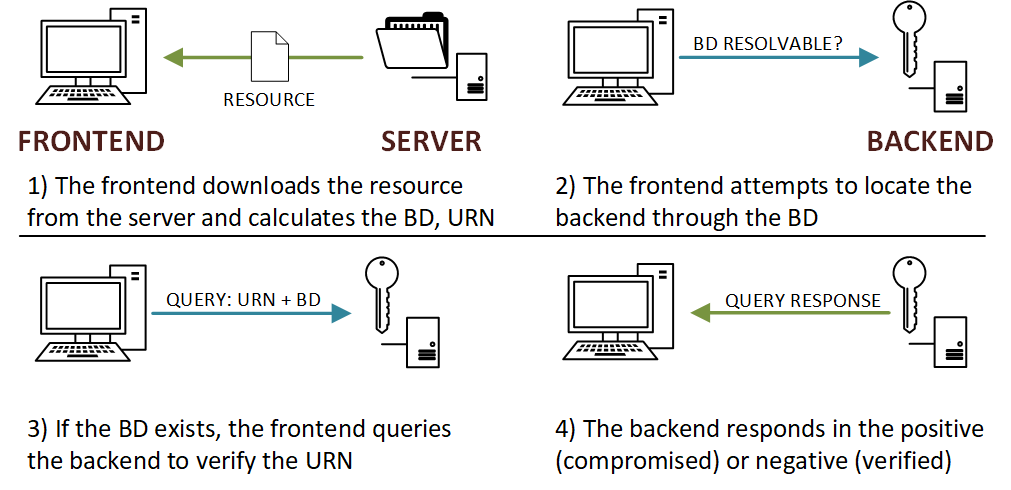
\includegraphics[width=\linewidth]{figs/hc/haschk-overview.png}
    \caption{A high level overview of the (generic) automated checksum
    verification process beginning when a user downloads a
    resource.} \label{fig:protocol}
\end{figure}

\figref{protocol} gives a high level overview of the HASCHK protocol.
Initially, when a user finishes downloading a resource from the provider's
server, the frontend runs the resource's contents through the SHA-256 hashing
function, yielding a 256-bit digest. Any hashing function can be used so long as
it is pre-image and collision resistant~\cite{Rogaway}. This digest is used to
construct a hash-based Uniform Resource Name~\cite{draft-URN} (URN) uniquely identifying the
resource. Additionally, a Backend Domain (BD) is derived from the domain name of
the server. The frontend uses the BD in an implementation-dependent manner to
locate and query the backend, checking for the existence of the constructed URN
and essentially asking: \emph{``is this a compromised resource?''} If the URN is
found, a negative response is returned indicating a verified resource. If the
URN is not found, a positive response is returned indicating a compromised
resource.

If the query returns a positive response: (1) the user should be warned pursuant
to the recommendations of Akhawe et al~\cite{Akhawe} (avoid warning fatigue, be
invisible), Cherubini et al~\cite{Cherubini} (simple non-technical language,
secure default action), Modic et al~\cite{Modic} (issue warnings from a position
of authority), and others; (2) the download should be deleted, renamed, or
otherwise made inaccessible/quarantined by default; and (3) the user should
still be allowed to ``click through'' and override the warning and the default
quarantine behavior, though ideally this should be less convenient than the
default action~\cite{Cherubini}.

If the query returns a negative response, the frontend should indicate this
inconspicuously to mitigate the threat of warning/popup fatigue~\cite{Akhawe,
Cherubini} and habituation~\cite{Sunshine}. For example, our frontend
implementation simply changes its icon when downloads are successfully verified
and only issues popup warnings when compromised downloads are positively
identified.

To prevent false positives, integrity checking is skipped if the backend's
location is unresolvable or HASCHK is not properly deployed. Determining when
this is the case is implementation-dependent. To prevent false-negatives, when
HASCHK is properly deployed and a URN is not found during lookup, the backend
response will always be interpreted as positive. As a result, it is not possible
to only secure ``some'' resources on a server.

\subsubsection{Deriving the Backend Domain (BD)}

Before we can communicate with a provider's backend, we require some scheme to
locate it. We refer to this scheme as \emph{deriving the Backend Domain} (BD).
The BD is some identifier that allows the frontend to locate the backend. For
our Domain Name System (DNS) based implementation (below), the BD is the
Third-Level Subdomain (3LD) or Second-Level Domain (2LD) based on the server
URI's host subcomponent~\cite{RFC3986} and are queried in that order. \\

Example 1: an FTP frontend (\eg{ Filezilla, Transmit, et cetera}) downloading a
resource from an FTP server at
\texttt{ftps://un:pw@ftp.example1.com:8080/some/resource} has a host
subcomponent of \texttt{ftp.example1.com} and a BD of \texttt{ftp.example1.com}
or \texttt{example1.com}. \\

Example 2: a browser frontend (\eg{ Lynx, Google Chrome, Internet Explorer, et
cetera}) downloading a resource at \texttt{https://s4.l.cdn.example2.com/fl}
from a hyperlink on the page \texttt{https://dl.app.example3.com/index/page} has
a host subcomponent of \texttt{dl.app.example3.com} (\emph{not
\texttt{s4.ll.cdn.example2.com}}) and a BD of \texttt{app.example3.com} or
\texttt{example3.com}. \\

It is important that the right BD is derived to ensure correct operation of the
protocol. This concern is implementation-dependent. Specifically, in the case of
the browser frontend in example 2 (above), the BD is not derived from the
resource's URI directly but from the URI of the HTML page containing the
hyperlink pointing to that resource. This prevents an adversary from trivially
fooling HASCHK by, for instance, replacing
\texttt{https://s4.l.cdn.example2.com} with a hyperlink pointing to
\texttt{https://attacker.com} and hosting a conforming HASCHK backend that
would cause the frontend to respond with a false negative.

Further, depending on the implementation, a frontend or backend may not be using
URIs and DNS to transact information over the internet at all. An example of
this is a purely Distributed Hash Table (DHT) based backend. In such a case, any
derivation algorithm (or no derivation at all, \eg{ the BD is hardcoded}) can be
used as long as correct operation of the protocol is ensured.

\subsubsection{Constructing Uniform Resource Names (URN)}

To ensure the integrity of arbitrary resources, we require some method to
uniquely and durably identify those resources. We accomplish this through the
adoption of the informal IETF draft for the construction of hash-based
\emph{Uniform Resource Names} (URNs)~\cite{draft-URN}, which the frontend
follows when calculating URNs for each resource downloaded. Through whatever
implementation-specific method, the backend must ``advertise'' or allow lookups
against a set of expected URNs corresponding to the resources hosted on the
provider's server, even if those resources have unstable access paths or URIs;
\eg{, when resources are hosted externally, on download mirrors, on CDNs, et
cetera}. This requirement is satisfied by implementations combining URNs with
the BD, thus durably associating the URNs calculated in the frontend with the
URNs advertised by a provider's backend regardless of where the corresponding
resources are hosted on the provider's server.

Since the backend advertising URNs is \emph{never} co-hosted alongside the
system that distributes the corresponding resources---like a web or FTP
server---HASCHK retains the ability to protect users from dangerous downloads
\emph{even when the system distributing the resource has been completely
compromised}. This is not true of prior approaches to automated checksum
verification of arbitrary resources~\cite{Cherubini}.

\section{Implementation} \label{sec:hc-implementation}

We implement a proof-of-concept HASCHK frontend as a Google Chrome extension.
To demonstrate the general applicability of our approach, our frontend currently
works with two backends: (1) directly with DNS via Google's JSON API for DNS
over HTTPS (DoH) and (2) indirectly with DHT (Ring OpenDHT) via a local
Representational State Transfer (REST) API we designed to mimic the response
syntax of Google's DoH JSON API. Other candidate backends include storage
clusters, relational and non-relational databases, and any high availability
key-value store.

Our extension operates following the high level overview in \figref{protocol}
with some key implementation-specific functionality that we explore in the
remainder of this subsection. After the user initiates a download either
directly (\eg{ typing a URI manually}) or by following a hyperlink, our
extension, having observed the initial web request, associates that request with
the new download item. The original request may have directly triggered the
download or the download may have been triggered after one or more redirections.
Our extension derives the correct BD in both cases (see below). At this point,
if the backend does not exist or does not conform to the protocol, the protocol
terminates. Otherwise, after the download completes, a URN is calculated and
combined with the BD to make a final query to the backend. In effect, this query
asks: \emph{is this resource compromised?} If the response to the query is
negative (\ie{ a DNS TXT record or DHT data value}), the extension considers the
resource validated. On the other hand, if the response to the query is positive
(\ie{ no record found or bad data value returned}), the extension considers the
resource compromised, deletes the resource file, and warns the user.

In keeping with UX suggestions of prior work, our extension is virtually
transparent to end users in the common case that a download is successfully
verified by a provider's backend or when HASCHK has not been properly
deployed by a provider. However, in the relatively uncommon case that a resource
is deemed compromised, the extension will delete the file and alert the user
with the primary option to ``dismiss'' the alert, mimicking Chrome's own highly
effective dangerous download warning~\cite{ChromeClickThrough}. Specifically:
the user has the option of clicking through the warning via a low-key secondary
interface where they can force the extension to ignore the compromised nature of
the resource \emph{the next time it is downloaded}, forcing the user to trigger
the download again. This inconvenience, favoring users' security over choice, is
in keeping with the recommendations of prior work regarding security warning UX
(see \secref{hc-motivation}).

As no JavaScript OpenDHT client implementation exists, we developed a REST API
to facilitate communication between our extension and the Ring OpenDHT network
via HTTP and JSON. In a production implementation, a JavaScript OpenDHT client
would be baked directly into the extension.

Deploying the DNS backend is as simple as adding certain TXT records to our DNS
zone. This is a straightforward operation. Similarly, deploying the DHT backend
requires adding certain key-value pairs to the OpenDHT network, which is
trivial. Moreover, both DNS and DHT backends are performant and highly
available. The Ring OpenDHT network is also free to use. In the case of DNS, the
vast majority of web-facing providers and IT teams are already using it, already
pay for their own DNS zones, and are already quite familiar with configuring and
managing them. Hence, no exotic secondary backend system is required for
providers with web servers. Additionally, we argue updating the URNs stored by
these backends automatically---by integrating a URN calculation and record
insertion/update step into a modern development toolchain or resource deployment
pipeline---is relatively low-effort and straightforward for providers.

No application or website source code changes, costly user-facing server or web
infrastructure customizations, or modifications to web standards are needed to
enable our extension to protect a provider's resources. Given a production-ready
implementation of our frontend---coupled with the near ubiquitous adoption of
DNS---HASCHK (with a DNS backend) could be deployed immediately by interested
providers.

\subsection{URNs, BDs, and Fallthrough in Google Chrome}

BD derivation in the browser is non-trivial. Users can initiate downloads
through clicking links inside \emph{and outside} the browser (\eg{ in an email
application}), through asynchronous JavaScript, and by entering URIs into the
browser manually. To catch these and other edge cases, we implement our
extension using the WebRequest API~\cite{ExtensionAPI}, which allows us to
monitor all navigation events, collate redirects into an interrogable chain of
requests, and associate new download items with the URI where they were
originally initiated.

To query the backend, we: (1) BASE32 encode the resource's URN. (2) Divide the
112-character result into two 56-character strings \texttt{C1} and \texttt{C2}.
(3) We calculate the BD, which is either the 3LD and 2LD from
\texttt{details.originUrl}. We choose by issuing up to two queries of the form
\texttt{AL.BD}, where the Application Label (AL) is the constant string
\texttt{\_haschk}, looking for a response containing the value \texttt{OK}. We
first query the 3LD as BD and, if we do not receive the proper response there,
query the 2LD as BD. If the proper response is not received from either query,
the extension assumes HASCHK has not been properly deployed and terminates.
(4) Otherwise, concatenating C1, C2, AL, and BD, we issue a query of the form
\texttt{C1.C2.AL.BD}, again looking for a response containing \texttt{OK}
(negative) or that the query was not found (positive).

To handle redirection, we use Chrome's Web Request API to associate redirected
requests with one another. The originating request's \texttt{origin} at the top
of this chain is used to derive the BD using the \texttt{details.originUrl} and
\texttt{details.documentUrl} properties (also avoiding iframe issues). This
prevents an adversary from trivially fooling HASCHK by replacing a legitimate
hyperlink with a malicious one. A naive implementation might use the
\texttt{DownloadItem.referrer} property to derive the BD, since it should be
populated with the originating URL. Unfortunately, this property can be
manipulated with one or more redirections causing the BD to point into the
attacker's DNS zone. If the attacker properly deploys a HASCHK backend, they
could then trivially force false negatives.

Keeping a chain of associated requests also allows us to implement
``fallthrough'' functionality where, if the original request at the head of the
chain has not deployed HASCHK, the extension can walk the chain, checking
each point of redirection for a proper HASCHK deployment. This ensures URL
shorteners and other redirection services do not trigger false positives.

\section{Evaluation} \label{sec:hc-evaluation}

\subsection{Security Goals and Threat Model}

The goal of HASCHK is to ensure the integrity of arbitrary resources
downloaded over the internet, even in the case where the system hosting those
resources is completely compromised. Given a HASCHK-aware client and a
resource provider with a conforming backend, the user must be automatically
warned whenever what they are downloading does not match a corresponding
authoritative checksum. Given proper deployment, HASCHK should, to whatever
extent possible, operate without issuing false negatives, \ie{ compromised
resources that do not trigger a warning}, or false positives, \ie{ benign
resources that do trigger a warning}.

We consider the following entities: (1) a HASCHK-aware client as the
\emph{frontend}, (2) a \emph{server} (or servers) as the distribution system
hosting the \emph{resource}, and (3) a separate high availability system
implementing HASCHK as the \emph{backend}. Specifically, we consider a
\emph{generic frontend} that might be any web-facing software, such as
FileZilla, and a \emph{browser frontend} such as Google Chrome or Mozilla
Firefox.

For a generic frontend, we assume the adversary can make the server respond to a
resource request with any resource, including a compromised version of a
resource. We also assume the adversary can tamper with any other server
response, including adding, removing, or manipulating one or more checksums if
they appear.

For a browser frontend and web server, we contemplate two scenarios. From either
an existing tab/window or a new one, the user (1) directly enters the resource
URI into the browser, initiating a direct download or (2) navigates to an HTML
file (\emph{web page}) on the server containing a hyperlink pointing to the
resource. The user clicks this hyperlink to download the resource. This resource
is hosted on the same server as the web page or externally on a third party
server such as a CDN. Both are valid deployments in the context of HASCHK. We
assume the adversary can manipulate the resource and web page wherever they are
stored. The adversary may: (1) compromise the resource, (2) modify the hyperlink
to point to a compromised resource anywhere on the internet, and/or (3) add,
remove, or manipulate any checksums that appear on the web page or elsewhere.

Hence, we do not trust the integrity of the server's responses in any scenario.
We do, however, trust the integrity and authenticity of the backend's responses.
Further, we expect the backend to be highly available. In
\secref{hc-evaluation}, we go over the implications of a compromised backend.

As an aside, we consider here the standard non-HASCHK case where the resource
is co-hosted alongside a web page containing both a hyperlink pointing to the
resource \emph{and an authoritative checksum corresponding to the resource}. As
demonstrated throughout the paper, when a server co-hosting resources and
checksums is compromised, it is trivial to manipulate both checksum and
resource, rendering all forms of checksum verification irrelevant. Assuming
proper deployment, it is the goal of HASCHK to ensure this is never the case.

\subsection{Security and Performance}

To empirically evaluate our implementation, we launch a lightly modified version
of the popular open source research submission and peer review software, HotCRP
(version 2.102; see \cref{app:availability}). Our modifications allow anyone
visiting the site to interactively corrupt submissions and manipulate relevant
DNS entries at will.

For our evaluation, we upload 10 different PDFs to our HotCRP instance. Upon
their upload, HotCRP calculates and displays the unique checksum (a SHA-256
digest) of each PDF. After each PDF is uploaded, we immediately download it and
manually calculate a checksum locally, matching each to the checksum displayed
by the HotCRP software. Next, we utilize the custom functionality we patched
into HotCRP to populate our DNS backend with each file's expected URN.

After installing the frontend into our Google Chrome browser, we again download
each file. For each observed download, our extension indicates a ``safe''
judgement. We then utilize our patched functionality to add junk data onto the
end of each of the uploaded PDFs, thus corrupting them. We also modified HotCRP
so that it updates the displayed checksums to match their now-corrupted
counterparts.

Once again, we download each file. Our extension reports an ``unsafe'' judgement
(a true positive) for each corrupted PDF file. Calculating the local checksum
and checking it against the value reported by our HotCRP instance leads to a
match (a false negative; \ie{, the result of co-hosting}), defeating prior
approaches to both manual and automated checksum verification.

We run this experiment three times, each with different sets of PDFs and using
both the DNS and DHT based backends. We observe consistent results.

Finally, we utilize our patched functionality to test a ``redirection'' attack
where the hyperlink pointing to the correct PDF is replaced with a hyperlink to
a dummy malware file hosted in a distinct malicious DNS zone with conforming
HASCHK deployment. When an unsuspecting user clicks such a link, they expect
to download the PDF document from HotCRP but are instead navigated to a PHP
script that redirects the request one or more times before landing on the dummy
malware file. This process corrupts Chrome's \texttt{DownloadItem.referrer}
property. Even in this case, our implementation correctly flags this download as
suspicious as the download begins, successfully warning the user.

While evaluating our implementation, we observe no additional network load or
CPU usage with the extension loaded into Chrome. Measurements are taken using
the Chrome developer tools. Intuitively, this makes sense given the lightweight
nature of the cryptographic operations involved.

We also consider the implications of a compromised backend, such as if an
attacker tampers with the provider's DNS server or its response. Since we trust
the integrity and authenticity of responses from the backend, this is ultimately
outside our threat model. However, in the case of a compromised DNS zone by
itself, at worst the attacker can perpetuate a denial of service attack by
triggering false positives. Without compromising both the backend and the
distribution server, the attacker still cannot deliver compromised resources to
users. Further, we argue a provider has much bigger problems if their DNS zone
or other backend is compromised.

\subsection{Scalability and Deployment}

As HASCHK assumes a high availability backend, we conclude that the
scalability of HASCHK can be reduced to the scalability of its backend. We
are aware of no other obstacles to scalability beyond those inherited from the
underlying backend system.

Obviously, our DNS backend relies on DNS~\cite{DNS1}. DNS was not originally
designed to transport or store relatively large amounts of data, but the content
of our DNS TXT records are very small (usually two bytes or less). Further, the
URNs queryable via DNS request are exactly 112 characters, \ie{the length of a
BASE32 encoded URN}, and are divided into two 53 character labels, conforming to
DNS label length limits~\cite{DNS2}.

We are also unaware of any practical limitation on the number of resource
records a DNS zone file can support. A DNS server can host tens of thousands of
resource records in their backend file~\cite{DNS1, DNS2}. Moreover, several
working groups have considered using DNS as a storage medium for checksums/hash
output, so the concept is not novel. Examples include
securitytxt~\cite{draft-sectxt} and DKIM~\cite{DKIM}.

Additionally, using DNS as a backend does not add to the danger of amplification
and other reflection attacks on DNS; these are generic DNS issues addressable at
other layers of the protocol.

With the HotCRP demo, our entire resource deployment scheme consists of (1) the
addition of a new TXT entry to our DNS backend and (2) a new value published to
our DHT backend during the paper (resource) submission process. We argue
updating DNS record (or DHT value) during the resource deployment process is
simple enough for developers and providers to implement and presents no
significant burden to deployment. For reference, we implement the functionality
that automatically adds (and updates) the DNS TXT records advertising the URNs
of papers uploaded to our HotCRP instance in under 10 lines of JavaScript.

\subsection{Limitations}

While still effective, our extension would be even more effective if
Chrome/Chromium or the more general WebExtensions API allowed for an explicit
\texttt{onComplete} event hook in the downloads API. This hook would fire
immediately before a file download completes and the file becomes executable,
\ie{ has its \texttt{.crdownload} or \texttt{.download} extension removed}. The
hook would consume a \texttt{Promise}/\texttt{AsyncFunction} that kept the
download in its fully-downloaded but non-complete state until said
\texttt{Promise} completed. Ideally, this would allow an extension to alter a
download's \texttt{DangerType} property after some computation, prompting Chrome
to handle alerting the user using its Dangerous Download
UX~\cite{ChromeClickThrough}, which would have the advantage of communicating
intent through the browser's familiar and authoritative UI and prevent the
corrupted download from becoming immediately executable. Unfortunately, the
closest the Chrome WebExtensions API comes to allowing \texttt{DangerType}
mutations is the \texttt{acceptDanger} method on the downloads API, but it is
not suitable for our purposes because it can only be called after the download
completes while leaving the file in an accessible and executable state until the
method is eventually called.

Redirection services, like URI shortening apps, might still lead to false
positives even with the fallthrough functionality if a domain on the request
chain has deployed HASCHK. We view this as a rare scenario, and it does not
violate HASCHK's security guarantees. Further, our extension does not work
for PDFs and other downloads handled directly by the browser. And, given the
topology of the webrequest API, iframes and similar elements may require special
consideration beyond examining \texttt{details.documentUrl}.

Additionally, not all servers/backends on the internet use DNS, and our
extension does not support downloads made that bypass DNS. In future work, our
DHT backend would be able to handle such downloads. Further, our extension keeps
1000 requests in memory so that they can be mapped to download items later in
time. This might be vulnerable to attacks involving excessive redirection and
overflow.


\chapter{Conclusion} \label{chp:conclusion}

The conventional wisdom is that securing data at rest requires one must pay the
high performance overhead of encryption with AES is XTS mode. This work shows
that technological trends overturn this conventional wisdom: log-structured file
systems and hardware support for secure counters make it practical to use a
stream cipher to secure data at rest. We demonstrate this practicality through
our implementation of StrongBox which uses the ChaCha20 stream cipher and the
Poly1305 MAC to provide secure storage and can be used as a drop-in replacement
for dm-crypt.

Our empirical results show that under F2FS---a modern, industrial-strength
Log-structured file system---StrongBox provides upwards of $2\times$ improvement
on read performance and average $1.27\times$ improvement on write performance
compared to dm-crypt. Further, our results show that F2FS plus StrongBox
provides a higher performance replacement for Ext4 backed with dm-crypt. We make
our implementation of StrongBox available open source so that others can extend
it or compare to it.\footnote{\StrongBoxURI} Our hope is that this work
motivates further exploration of fast stream ciphers as replacements for AES-XTS
for securing data at rest.

Further, this work advocates for a more flexible approach to FDE where the
storage system can dynamically adjust the tradeoffs between security and
latency/energy. To support this vision of agile encryption, we proposed an
interface that allows multiple stream ciphers with different input and output
characteristics to be composed in a generic manner. We have identified three
strategies for using this interface to switch ciphers dynamically and with low
overhead. We have also proposed a quantification framework for determining when
to use one cipher over another. Our case studies show how different strategies
can be used to optimize for different goals in practice. We believe that agile
encryption will become increasingly important as successful systems are
increasingly required to balance conflicting operational requirements. We hope
that this work inspires further research in achieving this balance. Our work is
publicly available open-source\footnoteref{note1}.

When it comes to data in motion---specifically, downloading arbitrary resources
over the internet---it is indeed a risky endeavor. Resource integrity and other
Supply Chain Attacks are becoming more frequent and their impact more widely
felt. In this work, we showed that the de facto standard for protecting the
integrity of arbitrary resources on the internet---the use of
\emph{checksums}---is insufficient and often ineffective. We presented HASCHK, a
practical resource verification protocol that automates the tedious parts of
checksum verification while leveraging pre-existing high availability systems to
ensure resources and their checksums are not vulnerable to co-hosting. Further,
we demonstrated the effectiveness and practicality of our approach versus
real-world resource integrity attacks in a production application.

The results of our final evaluation show that our approach is more effective
than checksums and prior work mitigating integrity attacks for arbitrary
resources on the internet. Further, we show HASCHK is capable of guarding
against a variety of attacks, is deployable at scale for providers that already
maintain a DNS presence, and can be deployed without fear of adversely affecting
the user experience of clients that are not HASCHK-aware. Though not a panacea,
we believe our protocol significantly raises the bar for the attacker. We intend
to continue developing our extension and we make it available to a wide audience
(see \cref{app:availability}).

\section{Future Work}

As it stands now, our StrongBox and SwitchCrypt implementations are single
threaded. The cryptographic systems we compared to StrongBox and SwitchCrypt and
all multi-threaded, perhaps making our performance wins more significant. What
performance gains (i.e. more slack) might be available if we parallelize
portions of StrongBox and SwitchCrypt source? Examples include: 1) given that
nuggets are all independent agents, new switching strategies might be developed
that leverage any speedups in parallelizing the encryption and decryption
processes and 2) garbage collection and cipher switching can happen in
background worker threads and could even leverage a scheduler and 3) StrongBox
and SwitchCrypt could be integrated into F2FS directly, sharing its
threading/scheduling model in a production implementation; currently, StrongBox
and SwitchCrypt are implemented on top of the BUSE emulation device.

\renewcommand\thechapter{A}
\chapter{Code Availability} \label{app:availability}

This appendix provides links for the StrongBox I and StrongBox II source code.
The two libraries/APIs that our StrongBox implementations rely on are
additionally provided. Note that resource locations, URLs, frameworks,
interfaces, etc. will likely change overtime, while this text remains static.

You can find instructions on how to build, test, and modify the StrongBox source
in the provided README documentation linked below.

\begin{table}
    \centering
    \caption{Provides URLs for the products yielded and/or used by this research.}
    \begin{tabular}{|r|c|l|l}
        \cline{1-3}
        \textbf{Project Source} & \textbf{Language} & \textbf{URL} & \\
        \cline{1-3}
        StrongBox I Source & C & https://github.com/research/buselfs-public & \\
        StrongBox II Source & C & https://github.com/research/buselfs2-public & \\
        SBD Merkle Tree Implementation & C & https://github.com/IAIK/secure-block-device & \\
        Block Device in User Space (BUSE) & C/Shell & https://github.com/acozzette/BUSE & \\
        \cline{1-3}
    \end{tabular}
\end{table}



% Format a LaTeX bibliography
\clearpage
\addcontentsline{toc}{chapter}{Bibliography}
\begin{singlespace}
    \printbibliography
\end{singlespace}

% Figures and tables, if you decide to leave them to the end
%\input{figure}
%\input{table}

\end{document}
